
\lhead[{\bfseries \thepage}]{ \rightmark}
\rhead[Resum de la tesi]{\bfseries \thepage}

%\markboth{Resumen de la tesis}{Resumen de la tesis}
%\addcontentsline{toc}{part}{Resumen de la tesis} 
\label{partIII}

%\begin{comment}
 \newcounter{betasect}

 \renewcommand\thesection{%
 \ifnum\value{betasect}=1%
A%%
 \else
\ifnum\value{betasect}=2%
B%%
\else
\ifnum\value{betasect}=3%
C%%
\else
\ifnum\value{betasect}=4%
D%%
\else
 \arabic{section}%%
 \fi\fi\fi\fi}%

 \newenvironment{asection}{%
 \setcounter{betasect}{1}%%
 }{%
 \setcounter{betasect}{0}%%
 }%

 \newenvironment{bsection}{%
 \setcounter{betasect}{2}%%
 }{%
 \setcounter{betasect}{0}%%
 }%
%\end{comment}


\setcounter{section}{0}

\chapter*{Recerca de la producció associada de bosó de Higgs i un quark top amb dos leptons i tau hadrònic en l'estat final}
\addcontentsline{toc}{chapter}{Resum de la tesi} 
\label{chap:resumen_val}

El Model Estàndard (SM) de la física de partícules és una teoria notablement exitosa, 
però també manifesta limitacions significatives. Aquest model unifica totes les partícules 
elementals que constitueixen l'univers conegut en una teoria única. Dins d'aquest marc, 
el quark $\text{top}$ i el bosó de Higgs desperten un interés especial, ja que poden 
contribuir a respondre algunes de les qüestions encara pendents. Aquesta tesi es 
centra en l'estudi d'ambdues partícules i la seua interacció. El
marc teòric per a l'estudi de la física d'aquestes partícules es presenta a
la Secció~\ref{chap:resumen_val:Teoria}.

Per dur a terme aquest estudi, s'han utilitzat dades de col·lisions protó--protó ($\Pproton \Pproton$) amb una 
lluminositat integrada de $140$$\text{fb}^{-1}$, a una energia de centre de masses de 
$13$~TeV, recopilades pel detector ATLAS durant el Run 2 del Gran Col·lisionador 
d'Hadrons (LHC) l'Organització Europea per a la Recerca Nuclear (CERN). L'ATLAS 
és el detector més gran de l'LHC, el més potent accelerador de partícules del 
món. El marc experimental en el qual s'emmarca aquest treball es descriu a la Secció 
\ref{chap:resumen_val:Exp}. La recopilació de les dades, la generació de simulacions 
de Monte Carlo, i la reconstrucció i identificació dels objectes físics són descrits a
la Secció~\ref{chap:resumen_val:Dades_i_Reco}.

El bosó de Higgs fou descobert pels experiments ATLAS~\cite{20121_ATLAS_HiggsDiscovery} 
i CMS~\cite{201230_CMS_HiggsDiscovery} en 2012 i, en conseqüencia, va obrir un nou camp d'exploració en la física 
de partícules. Per comprendre millor l'SM, és d'un gran interés determinar l'acoblament de Yukawa 
del bosó de Higgs amb el quark $\text{top}$ (\yt). Aquest quark és la partícula fonamental més massiva 
i, per tant, presenta l'acoblament més fort amb el bosó de Higgs.

La mesura directa de \yt només és possible a l'LHC a través de dues produccions associades 
del bosó de Higgs: amb un parell de quark--antiquark de $\text{top}$ (\ttH) i amb un unic quark $\text{top}$ 
juntament amb un partó addicional (\tHq). Mentre que el \ttH només permet determinar la 
magnitud de \yt, l'única manera de mesurar simultàniament el seu signe i la seua magnitud és mitjançant la
 producció \tH~\cite{Demartin:2015uha}. L'observació d'un excés d'esdeveniments de senyal en 
 comparació amb la predicció de l'SM podria ser una evidència de nova física en termes de violació 
 de \CP a l'acoblament \yt.
 
 En aquest treball, es presenta una cerca de la producció \tHq a l'estat final definit 
per dos leptons lleugers carregats (electrons o muons) i un leptó $\Ptau$ que es desintegra 
de manera hadrònica. Aquesta configuració es coneix com a canal \dileptau.
Aquesta búsqueda presenta un repte a causa de l'extremadament menuda secció eficaç del procés \tHq en general,
i sobretot pel canal final \dileptau, que representa només el 3.5\% de la producció total de \tHq.

Per distingir els esdeveniments de senyal \tHq dels de fons s'han fet servir tècniques d'aprenentatge automàtic. 
En concret, s'han utilitzat arbres de decisió potenciats (BDT) per definir tant les regions enriquides de senyal com les regions 
de control que limiten els processos de fons més importants. Els fons rellevants inclouen la producció de parells 
de quark--antiquark de $\text{top}$ en solitari i amb un bosó addicional (\ttbar, $t\bar{t}H$, $t\bar{t}W$ i $t\bar{t}Z$) i 
el bosó $Z$ juntament amb \textit{jets}\footnote{Un jet es refereix a un feix concentrat de partícules produïdes 
quan un quark o gluó es desintegra i s'hadronitza, donant lloc un grup de partícules detectables que emergeixen
en una direcció similar formant un con.}.


A més, per ajudar a identificar els esdeveniments de senyal dins les dades, la reconstrucció de l'esdeveniment juga 
un paper crucial. En situacions en què els leptons lleugers tenen la mateixa càrrega elèctrica, no és possible 
determinar a priori quin leptó prové del bosó de Higgs i quin del quark $\text{top}$. Atés aquest fet s'ha 
desenvolupat una eina basada en un BDT per assignar exitosament l'origen. 

S'aconsegueix una supressió significativa dels esdeveniments de fons, imposant requisits estrictes d'identificació i aïllament 
per als electrons i muons. Al mateix temps, es demana als taus hadrònics que superen un discriminador basat en xarxes 
neuronals recurrents per reduir les identificacions errònies provinents dels jets.

Totes les ferramentes mencionades per a la recerca de processos \tH i el procediment per a l'anàlisi estan descrits a la 
Secció~\ref{chap:resumen_val:tHq}, on també es presenten i discuteixen els resultats.

%%%%%%%
%   Teoria   %
%%%%%%%
\section{Marc teòric}
\label{chap:resumen_val:Teoria}

\subsection{El Model Estàndard}
%https://www.quantamagazine.org/a-new-map-of-the-standard-model-of-particle-physics-20201022/
L'SM és un marc teòric que descriu els constituents 
bàsics de la matèria i les seues interaccions. És el model més àmpliament acceptat i confirmat experimentalment 
en la física de partícules. La Figura~\ref{fig:resumen_val:Teoria:SM} recull totes les partícules fonamentals descrites per l'SM.

L'SM inclou dos tipus de partícules elementals: els fermions i els bosons.
Els fermions són partícules subatòmiques que segueixen les regles de l'estadística de Fermi-Dirac. 
Aquest tipus de partícula es caracteritza per tenir un espín semienter i per seguir el principi d'exclusió 
de Pauli, el qual estableix que dos fermions no poden ocupar el mateix estat quàntic simultaneament. 
Els fermions es divideixen en quarks i leptons. Ambdós tipus de fermions són els constituents bàsics 
de la matèria, però són diferents entre si.

\begin{figure}[h]
 	 \centering
 	  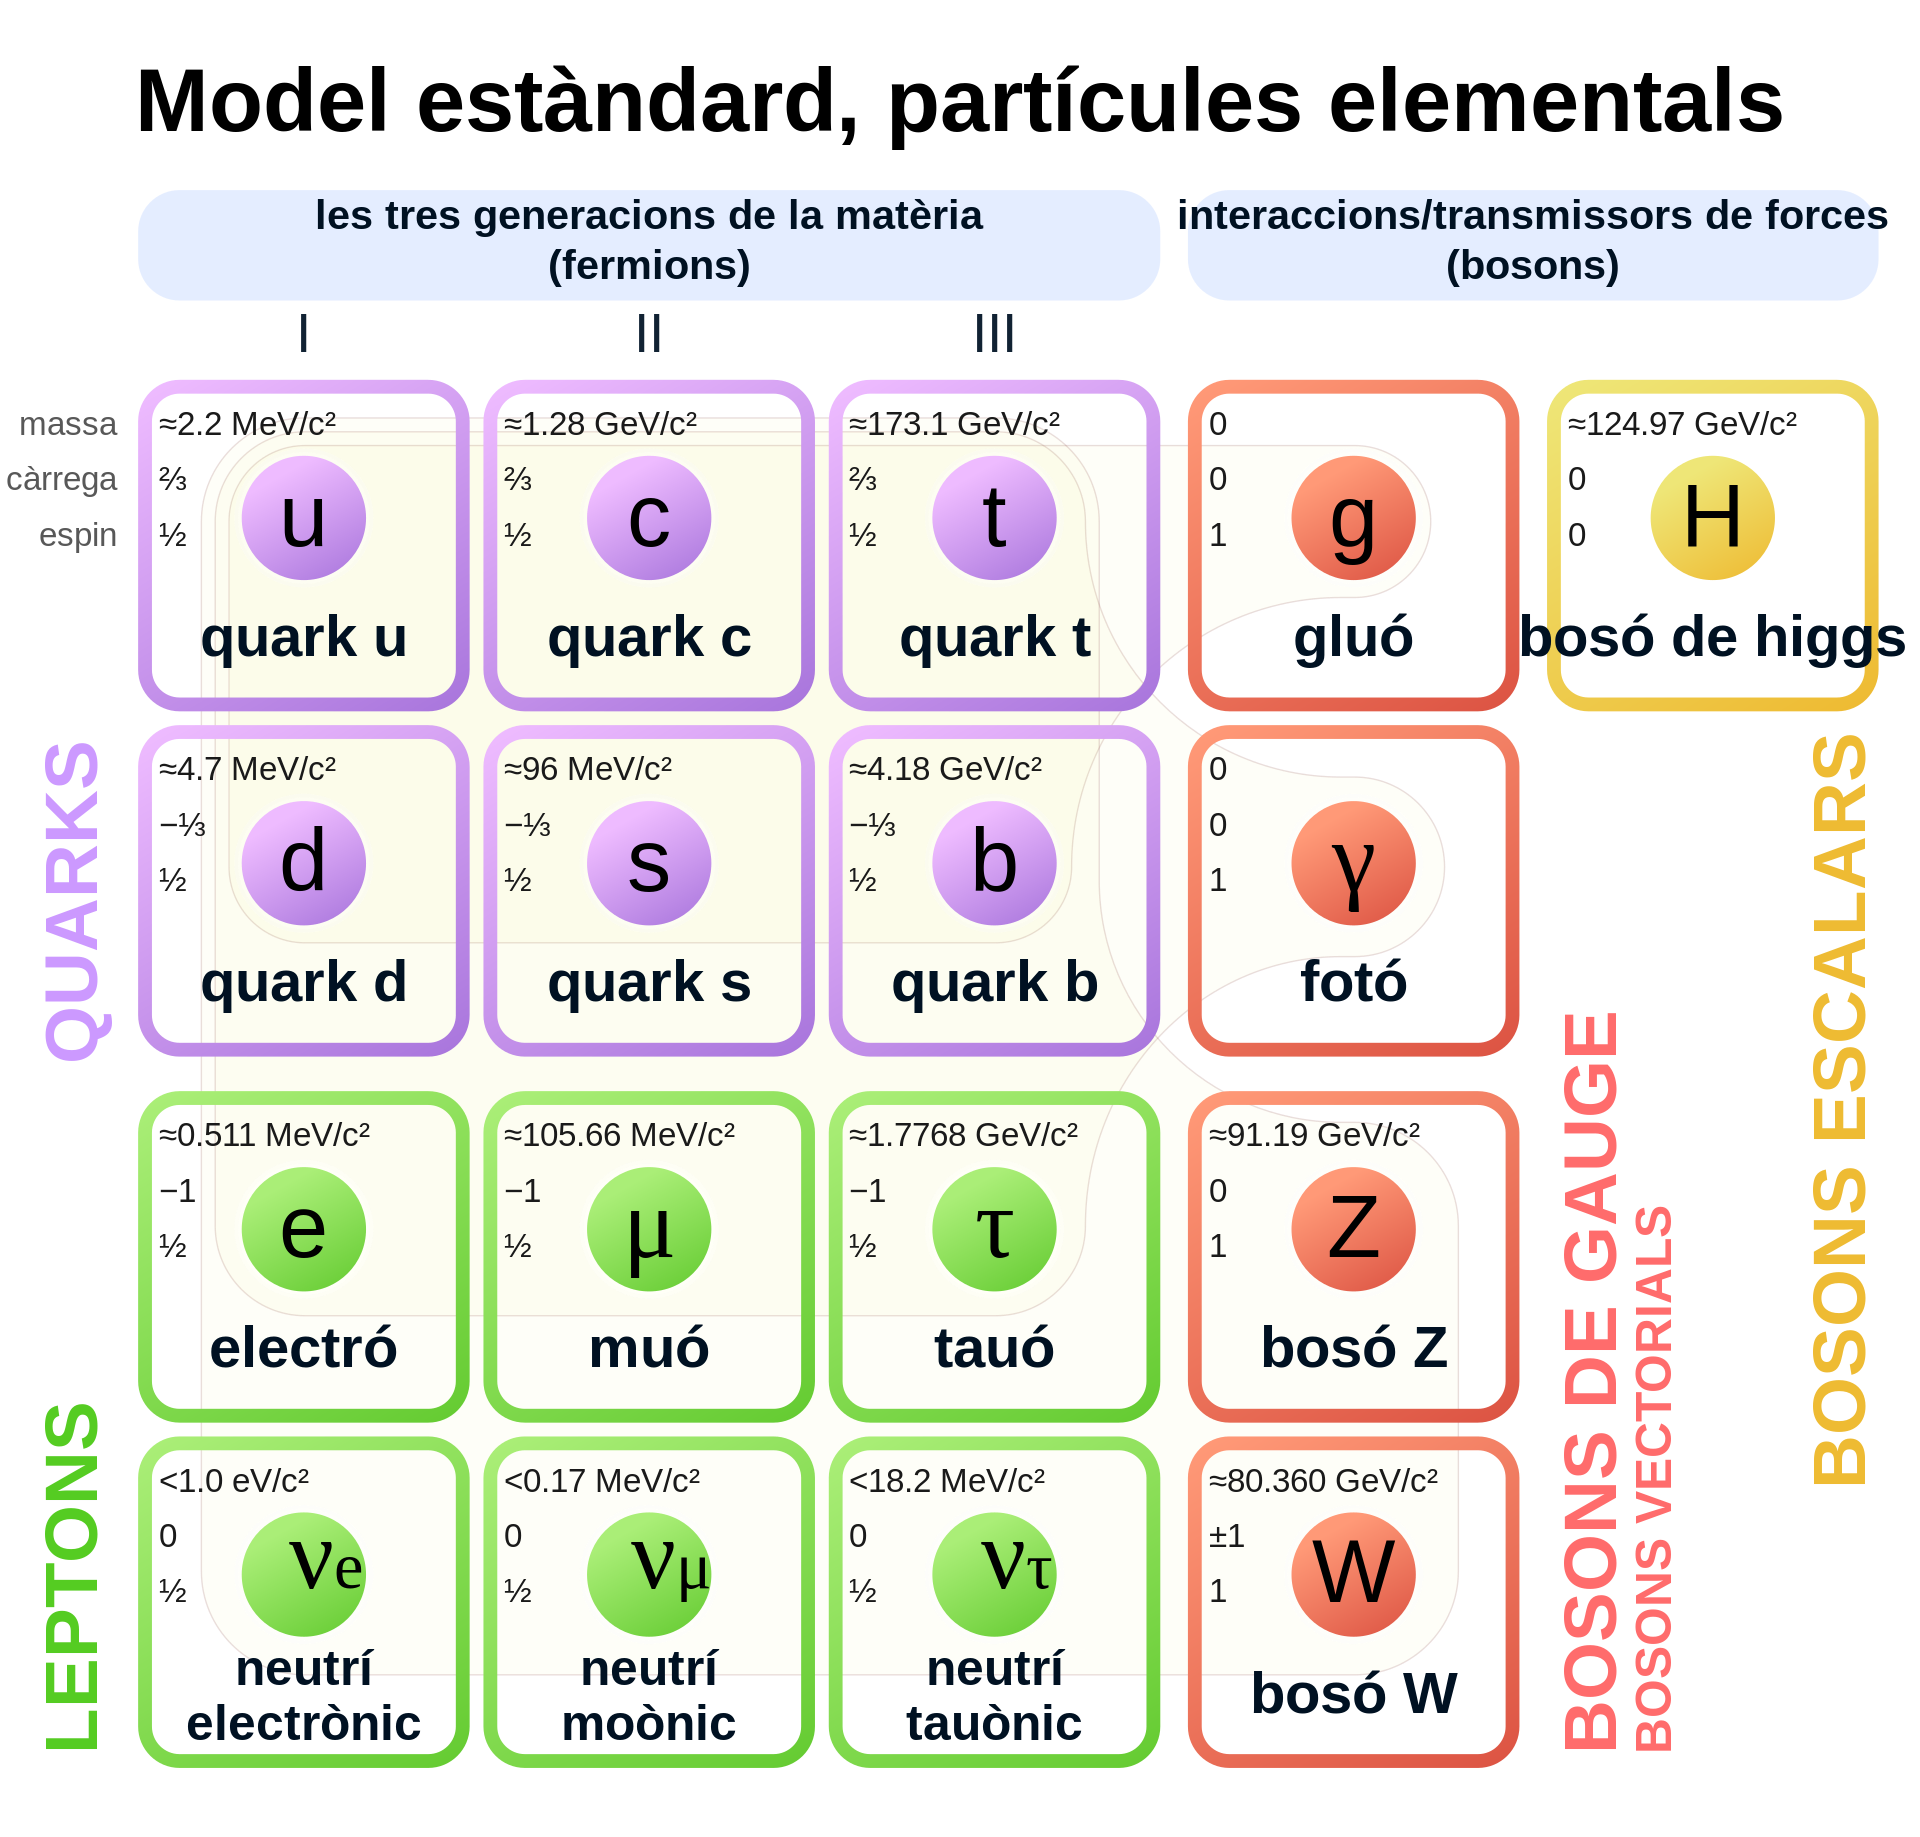
\includegraphics[width = 0.7\textwidth]{Chapter1/ZZ_Valencia_SM}
	  \caption{Model estàndard de les partícules elementals, amb les tres generacions de partícules de 
	  matèria, els bosons de gauge i el bosó de Higgs. Les superfícies en marró clar indiquen quins 
	  bosons (roig) s'acoblen a quins fermions (morat i verd)..} 
	\label{fig:resumen_val:Teoria:SM}
\end{figure}


D'una banda, els quarks són partícules que tenen càrrega elèctrica fraccionària. A més són la unitat fonamental 
dels protons i els neutrons. Aquestes partícules es combinen en grups per formar hadrons (mesons i barions). Els barions 
inclouen els protons i els neutrons, que són les partícules subatòmiques més abundants en la matèria. Els mesons tenen un 
nombre parell de quarks, la qual cosa fa que tinguen espín enter i siguen bosons. Els quarks es divideixen en sis ``sabors'' 
diferents: amunt, avall, encant, estrany, superior i inferior. La forma més habitual de referir-se a ells és pel seu nom en anglés: 
\textit{up}, \textit{down}, \textit{charm}, \textit{strange}, \textit{top} i \textit{bottom}.

D'una altra banda, els leptons ten càrrega elèctrica sencera i es classifiquen en leptons carregats (electró, muó i tauó, amb), que
tenen càrrega -1 i una massa relativament petita comparada amb altres partícules subatòmiques com els quarks,
i els neutrins (neutrí electrònic, neutrí muònic i neutrí tauònic), amb càrrega neutra i massa quasi nul·la.

Els altres elements que componen l'SM són els bosons, partícules amb espín enter que medien les 
interaccions fonamentals de la física. Els bosons de calibre (espín 1) són els responsables de descriure 
tres de les quatre forces fonamentals de la naturalesa\footnote{La gravetat queda fora de l'SM.}:

\begin{itemize}
	\item Interacció electromagnètica: Mediada pel fotó (\Pgamma), és la teoria que estudia 
	els fenòmens elèctrics i magnètics. Totes les partícules carregades interactuen entre si a 
	través d'aquesta força. Les principals característiques de la interacció electromagnètica són 
	el seu abast infinit i l'absència de massa dels seus portadors. En aquest sentit, és responsable de l'estabilitat 
	dels àtoms, ja que manté units els electrons en òrbita al voltant del nucli, i de la transmissió 
	de la llum i altres formes de radiació electromagnètica. La teoria que descriu aquesta interacció 
	es denomina electrodinàmica quàntica.
	
	\item Interacció nuclear feble: Mediada per dos bosons \PW (\PWplus i \PWminus) i el bosó \PZ. 
	Aquesta és responsable de la radioactivitat $\beta$, en la qual un neutró es descompon en un 
	protó, un electró i un antineutrí. També és la força a través de la qual té lloc la desintegració del quark top 
	en un quark \Pbottom i un bosó \PW. A més, la interacció nuclear feble és crucial en el procés 
	de fusió en les estrelles, on es combinen protons per formar elements més pesants. Les forces 
	nuclear feble i electromagnètica es descriuen simultàniament per la teoria electrofeble (EW).
	
	\item Interacció nuclear forta: Mediada pel gluó, és responsable de mantenir units els protons i 
	neutrons al nucli atòmic. És la interacció més forta de la naturalesa, però el seu abast d'acció 
	està limitat a distàncies subatòmiques. A causa del confinament per color de la teoria nuclear 
	forta, ni els gluons ni els quarks apareixen aïllats (excepte a altes energies). La teoria que descriu 
	aquesta interacció es diu cromodinàmica quàntica (QCD). Aquesta teoria, igual que l'electrodinàmica 
	quàntica i la teoria electrofeble, està basada en el formalisme de la teoria quàntica de camps.
\end{itemize}






%%%%%%%%%%%%%%%%%%%%%
%                 Top quark physics               % 
%%%%%%%%%%%%%%%%%%%%%
\subsection{La física del quark top}
\label{sec:resum:FisicaTop}
El quark top (\Ptop), o simplement top, és el quark de tipus up de la tercera generació de 
fermions. La seua característica més distintiva és la seua enorme massa, sent aquesta la més 
gran entre totes les partícules fonamentals. La seua existencia va ser postulada al 1973 
per Kobayashi i Maskawa~\cite{Kobayashi:1973fv} i es va observar per primera vegada al 
Tevatron a l'any 1995~\cite{CDF:1995wbb, D0:1995jca}.
Sovint, el quark top és considerat com una
finestra per a la nova física perquè proporciona un laboratori únic per provar la comprensió de l'SM.

La seua fenomenologia està determinada per 
la seua gran massa, deguda a la qual, la vida mitjana del quark top és la més curta entre totes les partícules de l'SM. 
($\tau_{\Ptop} = 5 \times 10^{-25}$s~\cite{Taylor:1998uk}). Això representa una 
oportunitat única per estudiar quarks en estat lliure, fet que és 
excepcional a causa del confinament de color. De fet, el quark top és l'únic 
quark que es pot investigar sense estar lligat. La seua vida mitjana també és 
menor que l'escala de temps de decorrelació d'espín 
($\mtop /\Lambda^{2}_{QCD} \sim 10^{-21}$~s~\cite{Mahlon:2010gw}), 
implicant que els estats del quark top conserven el seu estat d'espín des de 
la producció fins la desintegració.
D'aquest mode, les propietats del quark top, com la informació d'espín, es poden 
obtenir a través dels seus productes de desintegració i, per tant, mesurar-se.


A més, la gran massa del quark top propicia que consegüentment, aquesta partícula siga
l'única amb un acoblament  de Yukawa al bosó de Higgs (\yt) de l'ordre de l'unitat.  L'objectiu 
principal d'aquesta tesi és, precisament, l'estudi de la interacció entre el quark top 
i el bosó de Higgs per mesurar la seua secció eficaç de producció i ajudar a determinar 
si el \yt és el que prediu l'SM o si hi ha alguna fase que viola la simetria de \CP i 
afecta així al signe de l'acoblament Yukawa entre el Higgs i el top.

%%%%%%%%%%%%%%%%%%%%%
%                 Top quark mass                   %
%%%%%%%%%%%%%%%%%%%%%
La masa del quark top (\mtop) és un paràmetre lliure de l'SM; llavors, la teoria no prediu 
el seu valor i, per tant, aquest ha de ser determinat experimentalment. Els estudis més recents 
per a la mesura de la massa del quark top aboquen $\mtop = 172.76 \pm 0.30$~GeV~\cite{Workman:2022ynf}. %~\cite{pdgTop}.

%%%%%%%%%%%%%%%%%%%%%%%%%%
%                Top quark production at LHC               %
%%%%%%%%%%%%%%%%%%%%%%%%%%
Pel que respecta a la seua producció, l'LHC és conegut com una fàbrica de quarks 
top a causa de la seua capacitat per produir aquestes partícules. En aquest col·lisionador,
el quark top es produeix principalment a través de dos mecanismes: mitjançant QCD, en 
forma de parelles de quark top i anti-top (\ttbar), i mitjançant el vèrtex \Wtb de la interacció EW, on
es produeix un sol quark top en associació amb altres partícules. 
\begin{itemize}
	\item \ttbar: És la font més gran de producció de quarks top en col·lisions hadròniques.
		Aquest procés és un dels més importants a l'LHC, ja que permet estudiar amb precisió 
		les propietats del quark top. A més, a causa de la seua dominància en la producció, \ttbar 
		és també un fons rellevant en moltes anàlisis tal i com la d'aquesta tesi.
	\item Quark top en solitari: Aquest mecanisme té una secció eficaç tres vegades menor a 
		la de \ttbar i es produeix gairebé exclusivament a través del vèrtex \Wtb de la interacció EW. %És 
		%precisament per això que la producció de quark top en solitari és essencial per a obtenir 
		%informació sobre la interacció \Wtb i per a mesurar directament del terme $|V_{tb}|$ 
		%de la matriu CKM en col·lisionadors d'hadrons.	
		En primer ordre (LO), hi ha tres modes de producció per al quark top en solitari, sent el canal-$t$ 
		el mecanisme dominant a l'LHC amb aproximadament el 70\% de la secció eficaç d'aquest mode  
		a $\CM=13$~TeV. Els altres processos són el \schannel i la producció associada $\Ptop\PW$. 
		Només el canal-$t$  i la producció $\Ptop\PW$ són rellevants per a la producció d'un sol quark top.
		%a l'EW a l'LHC, ja que el \schannel encara no s'ha observat.	
\end{itemize}
Les produccions associades de quark top són processos importants per tal de mesurar l'acoblament 
del quark top amb les altres partícules de l'SM. El quark top en solitari es pot produir en associació 
amb altres partícules ($\Ptop X$) com els bosons \PZ, \PW, \Pgamma o \PHiggs. 
El tema d'aquesta tesi gira precisament al voltant d'una producció 
associada particular. Més concretament, la producció amb un bosó de Higgs (\tHq).

%%%%%%%%%%%%%%%%%
%                Top decay               %
%%%%%%%%%%%%%%%%%z
Pel que fa a la seua desintegració,  el quark top es desintegra quasi completament ($\sim 99.8\%$) 
a través del vèrtex \Wtb en un quark \Pbottom i un bosó \PW. Per això és habitual fer la classificació
segons la desintegració subsegüent del bosó \PW.  Per al \PWplus, les BR (fraccions de desintegració) 
per als diferents modes de desintegració són~\cite{Workman:2022ynf}:
\begin{align*}
	\PWplus &\rightarrow \Ppositron \Pneutrino_{e} 			&& (10.71 \pm 0.16)\% \\
	\PWplus &\rightarrow \APmuon \Pneutrino_{\mu} 			&& (10.63 \pm 0.15)\% \\
	\PWplus &\rightarrow \APtauon \Pneutrino_{\tau} 			&& (11.38 \pm 0.21)\% \\
	\PWplus &\rightarrow \Pquark \APquark \textrm{ (hadrons)}	&& (67.41 \pm 0.27)\% \\
	\PWplus &\rightarrow \textrm{invisible}					&& (1.4 \pm 2.9)\% 
\end{align*} 
Per als processos conjugats que involucren el \PWminus, les BR són les mateixes.


%%%%%%%%%%%%%%%%%%%%%
%            Higgs boson physics                %
%%%%%%%%%%%%%%%%%%%%%
\subsection{La física del bosó de Higgs}
\label{sec:resum:FisicaHiggs}
Després del quark top, el bosó de Higgs (\PH) o simplement Higgs és la partícula més massiva del 
SM amb una massa de $\mH = 125.25 \pm 0.17$~GeV~\cite{Workman:2022ynf}. La seua existència va ser 
teoritzada l'any 1964 per tres grups teòrics treballant independentment: Englert-Brout~\cite{PhysRevLett.13.321}, 
Higgs~\cite{PhysRevLett.13.508} i Guralnik-Hagen-Kibble~\cite{PhysRevLett.13.585}. 
%~\cite{pdgHiggs}

Els experiments ATLAS~\cite{20121_ATLAS_HiggsDiscovery} i CMS 
\cite{201230_CMS_HiggsDiscovery} de l'LHC van anunciar el descobriment
del bosó de Higgs en l'any 2012, la qual cosa va suposar un de les grans fites de l'SM.

%%%%%%%%%%%%%%%%%%%%%%%%%
%                Higgs production and decay              %
%%%%%%%%%%%%%%%%%%%%%%%%%
Els quatre processos més dominants per a la producció de bosons de Higgs en l'LHC
són:  fusió de gluons ($\Pgluon \Pgluon$F), fusió de bosons vectorials (VBF), Higgsstrahlung 
(VH), producció associada a parell de quarks ($q\bar{q}H$ i producció associada a un 
quark top i un Higgs ($tHX$). Per a una massa $\mH = 125.2$ GeV, les seccions eficaces de 
producció de Higgs són~\cite{LHCHiggsCrossSectionWorkingGroup:2016ypw}:


\begin{minipage}[t]{0.3\textwidth}
  \centering\raisebox{\dimexpr \topskip-\height}{%
  \includegraphics[width=\textwidth]{Chapter1/Pie_HiggsXSec}}
  %\captionof{figure}{}
  %\label{fig:Chap1:Higgs:Prod_and_BR:Prod}
\end{minipage}\hfill
\begin{minipage}[t]{0.7\textwidth}
\begin{flushleft}
\begin{flalign*}
	\sigma_{ggF}	&= 48.5_{-3.3}^{+2.2}\,\textrm{pb} \\
	\sigma_{VBF}	&= 3.78 \pm 0.05\,\textrm{pb} \\
	\sigma_{WH} 	&= 1.37\pm 0.03\,\textrm{pb} \\
	\sigma_{ZH} 	&= 0.89^{+0.04}_{-0.03}\,\textrm{pb} \\
	\sigma_{\ttH}	&= 0.5^{+0.03}_{-0.05}\,\textrm{pb} \\
	\sigma_{\bbbar H}	&=0.49^{+0.10}_{-0.11}\,\textrm{pb} \\
	\sigma_{tHX}	&= 0.09\pm 0.01\,\textrm{pb} 
\end{flalign*}
\end{flushleft}
\end{minipage}

El bosó de Higgs té una vida mitjana relativament curta\footnote{La més baixa després del quak top i els bosons EW.} 
($\tau_{\PH} = 1.6 \times 10^{-22}$~s~\cite{LHCHiggsCrossSectionWorkingGroup:2016ypw}) i, per tant, sempre es detecta 
a través dels seus productes de desintegració. Les seves fraccions de desintegració
segons la seua importància i assumint una $\mH=125.2$~GeV són~\cite{LHCHiggsCrossSectionWorkingGroup:2016ypw}:

\begin{minipage}[t]{0.4\textwidth}
  \centering\raisebox{\dimexpr \topskip-\height}{%
  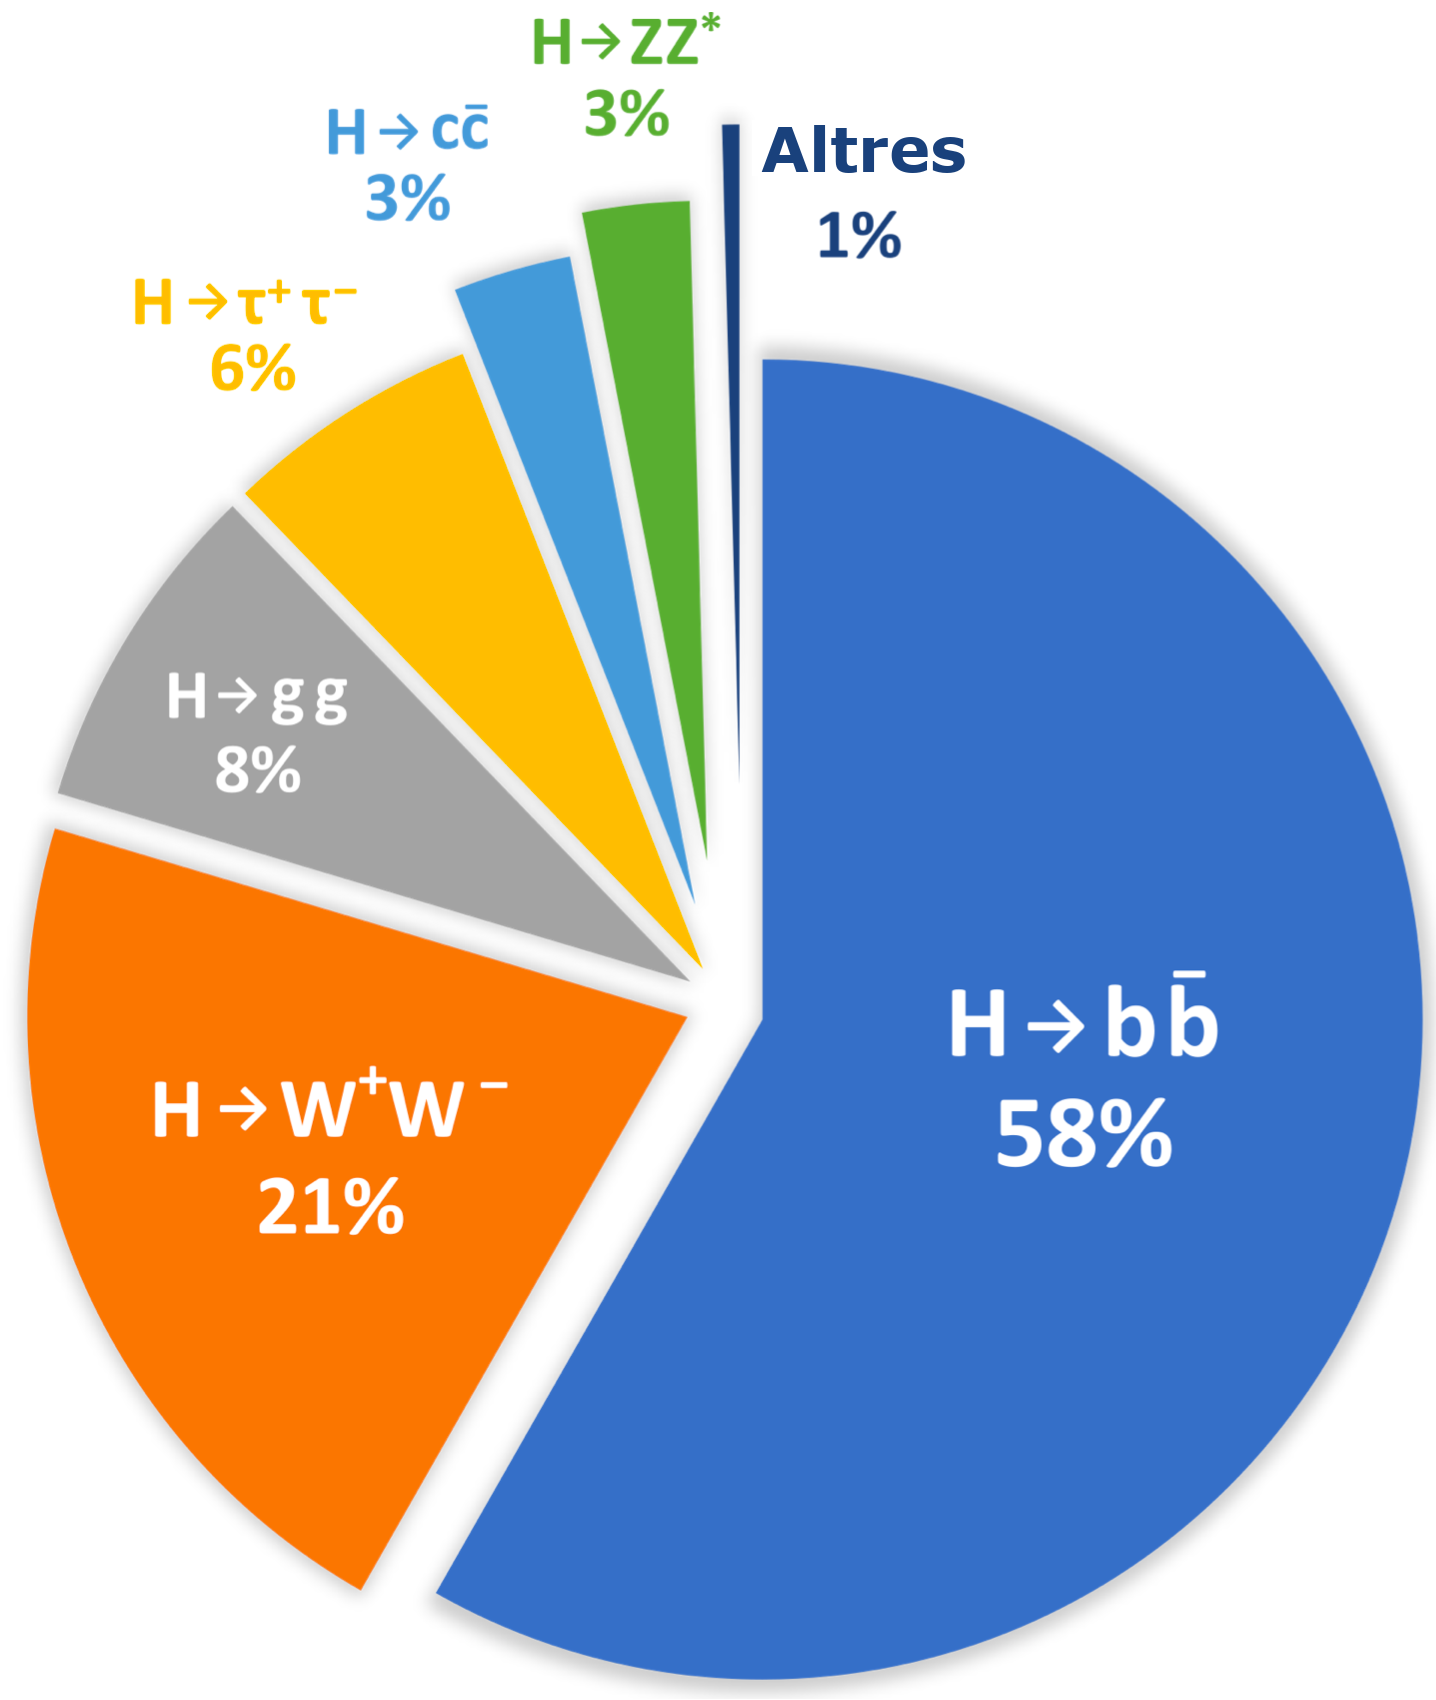
\includegraphics[width= 0.82\textwidth]{Chapter1/Pie_HiggsDecay_val}}
  %\captionof{figure}{}
  %\label{fig:Chap1:Higgs:Prod_and_BR:BR}
\end{minipage}\hfill
\begin{minipage}[t]{0.6\textwidth}
\begin{flushleft}
\begin{align*}
	\PHiggs &\rightarrow  \bbbar 			& (57.92 \pm 0.29)\% \\
	\PHiggs &\rightarrow  \PWplus\PWminus	& (21.70 \pm 0.11)\% \\
	\PHiggs &\rightarrow  \Pgluon \Pgluon 	& (8.17 \pm 0.26)\% \\ 
	\PHiggs &\rightarrow  \Ptauon\APtauon	& (6.24 \pm 0.03)\% \\
	\PHiggs &\rightarrow  \Pcharm \APcharm	& (2.888 \pm 0.014)\% \\ 
	\PHiggs &\rightarrow  \PZ\PZ			& (2.667 \pm 0.013)\% \\  
	\PHiggs &\rightarrow  \Pgamma \Pgamma	& (2.270 \pm 0.023)\% \\ 
	\PHiggs &\rightarrow  \Pmuon\APmuon	& (2.165 \pm 0.011)\% \\  
	\PHiggs &\rightarrow  \PZ \Pgamma		& (0.155 \pm 0.008)\% \\
	\PHiggs &\rightarrow \text{Altres}			& < 0.2 \%
\end{align*}
\end{flushleft}
\end{minipage}



%%%%%%%%%%%%%%%%%%%%%
%                Top-Higgs interplay              %
%%%%%%%%%%%%%%%%%%%%%
\subsection{Interacció entre el quark top i el bosó de Higgs}
Com que el quark top és la partícula més massiva, s'espera que \yt siga el més fort entre tots els acoblaments 
del bosón de Higgs amb fermions i, per tant, 
el seu estudi té una importància crucial, tal com es discuteix a les referències~\cite{Farina:2012xp} 
i~\cite{Biswas:2012bd}. S'espera que l'acoblament Yukawa estiga de l'ordre de la unitat:
\begin{equation*}
y_t = \frac{\sqrt{2} \cdot m_{\text{top}}}{v} = 2^{3/4} \sqrt{G_F} \cdot m_{\text{top}} \approx 0.995 \approx 1 \, ,
\end{equation*}
on $G_{F}$ és la constant. Aquest valor és molt més gran que els acoblaments dels altres quarks. 
Per comparació, $y_b \approx 0.025$ i $y_c \approx 0.007 \gg y_{s,d,u}$.

La producció d'una parella de quarks top juntament amb un bosó de Higgs (\ttH) és el 
principal mecanisme de producció associada d'aquestes dues partícules. El process \ttH permet 
mesurar el valor absolut de \yt. D'altra banda, amb una secció eficaç molt més baixa que \ttH, 
la producció del bosó de Higgs acompanyant un sol quark top (\tH) aporta informació valuosa, 
especialment pel que fa al signe del coupling de Yukawa. La producció de processos \tH en general
i \tHq en particular constitueix el tema central de la recerca descrita a aquesta tesi.   

L'associada producció \tH té lloc a través de tres tipus diferents de processos. En primer lloc, el canal-$t$, 
on el bosó de Higgs es radia desde el quark top o el bosó \PW (Figures~\ref{fig:Resum:tHq:Feynman_LO_top} i 
\ref{fig:Resum:tHq:Feynman_LO_W}, respectivament). En aquest canal, el top i el Higgs es creen juntament 
amb un quark addicional, donant lloc a la denominada producció \tHq. L'altre procés d'interés és la producción
\tWH, que consisteix en un procés \tW on el Higgs s'emiteix desde el quark top (Figura~\ref{fig:Resum:tHW:Feynman_LO}).
El tercer mode de producció és el canal-$s$. Aquest últim és poc relletvant degut a la seua petita secció eficaç.

\begin{figure}
\centering
 \begin{subfigure}{.29\textwidth}
  \centering
  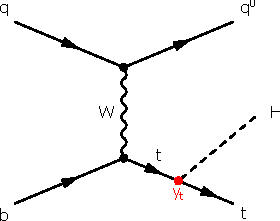
\includegraphics[width=.9\linewidth]{Chapter1/tHq_production_LO_Feynman_top}
  \caption{\tHq}
  \label{fig:Resum:tHq:Feynman_LO_top}
 \end{subfigure}%
 \begin{subfigure}{.29\textwidth}%
  \centering
  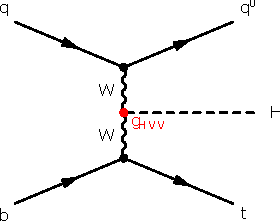
\includegraphics[width=.9\linewidth]{Chapter1/tHq_production_LO_Feynman_W}
  \caption{\tHq}
  \label{fig:Resum:tHq:Feynman_LO_W}
 \end{subfigure}%
 \begin{subfigure}{.29\textwidth}
  \centering
  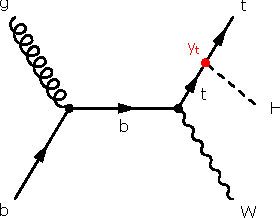
\includegraphics[width=.9\linewidth]{Chapter1/tHW_production_LO_Feynman}
  \caption{\tWH}
  \label{fig:Resum:tHW:Feynman_LO}
 \end{subfigure}%
    \caption{Representació dels diagrames de Feynman a LO per a \tH. A les figures (a) i (b) 
    es mostra el procés \tHq. Ací el bosó de Higgs s'acopla al quark top (a) o al bosó \PW (b). 
    A la figura (b), $g_{HVV}$ és el coupling del bosó de Higgs amb els bosons vectorials. 
    A la figura (c), es mostra la producció \tWH.}
    \label{fig:Resum:tHq:Feynman_LO}
\end{figure}
 
 
\subsubsection{Caracterització del bosó de Higgs en \tH i sensitivitat cap a \yt }

El Lagrangià efectiu que descriu l'acoblament de Yukawa entre el bosó de Higgs i el quark top 
per sota de l'escala de ruptura de la simetria EW és el següent~\cite{Demartin:2015uha}:

\begin{equation*}
\label{eq:Resum:Lagrangian:tHq:b}
\mathcal{L} = -\frac{\yt}{\sqrt{2}}\bar{\psi_{t}}[\text{cos}(\alpha)\kappa_{Htt} +  i\,\text{sen}(\alpha)\kappa_{Att} \gamma^{5}]\psi_{t}X_{0}\, .
\end{equation*}
Ací, $\psi_{t}$ i $X_{0}$ representen el quark top i el bosó de Higgs respectivament, 
i $\alpha$ és l'angle de mescla de \CP. Els paràmetres d'escala $\kappa_{Htt}$ i $\kappa_{Att}$ 
són adimensionals i reals.

La Figura~\ref{fig:Resum:xsec_vs_yt_tH_ttH} mostra la secció eficaç per a la producció 
$\Ptop X_{0}$ en el canal-$t$ com a funció de l'angle $\alpha$. Per a comparar, també 
es mostra la secció eficaç $\ttbar X_0$.  Ací $\Ptop X_{0}$ i $\ttbar X_{0}$ representen
respectivament els processos els \tH i \ttH.

\begin{figure}[h]
    \centering
    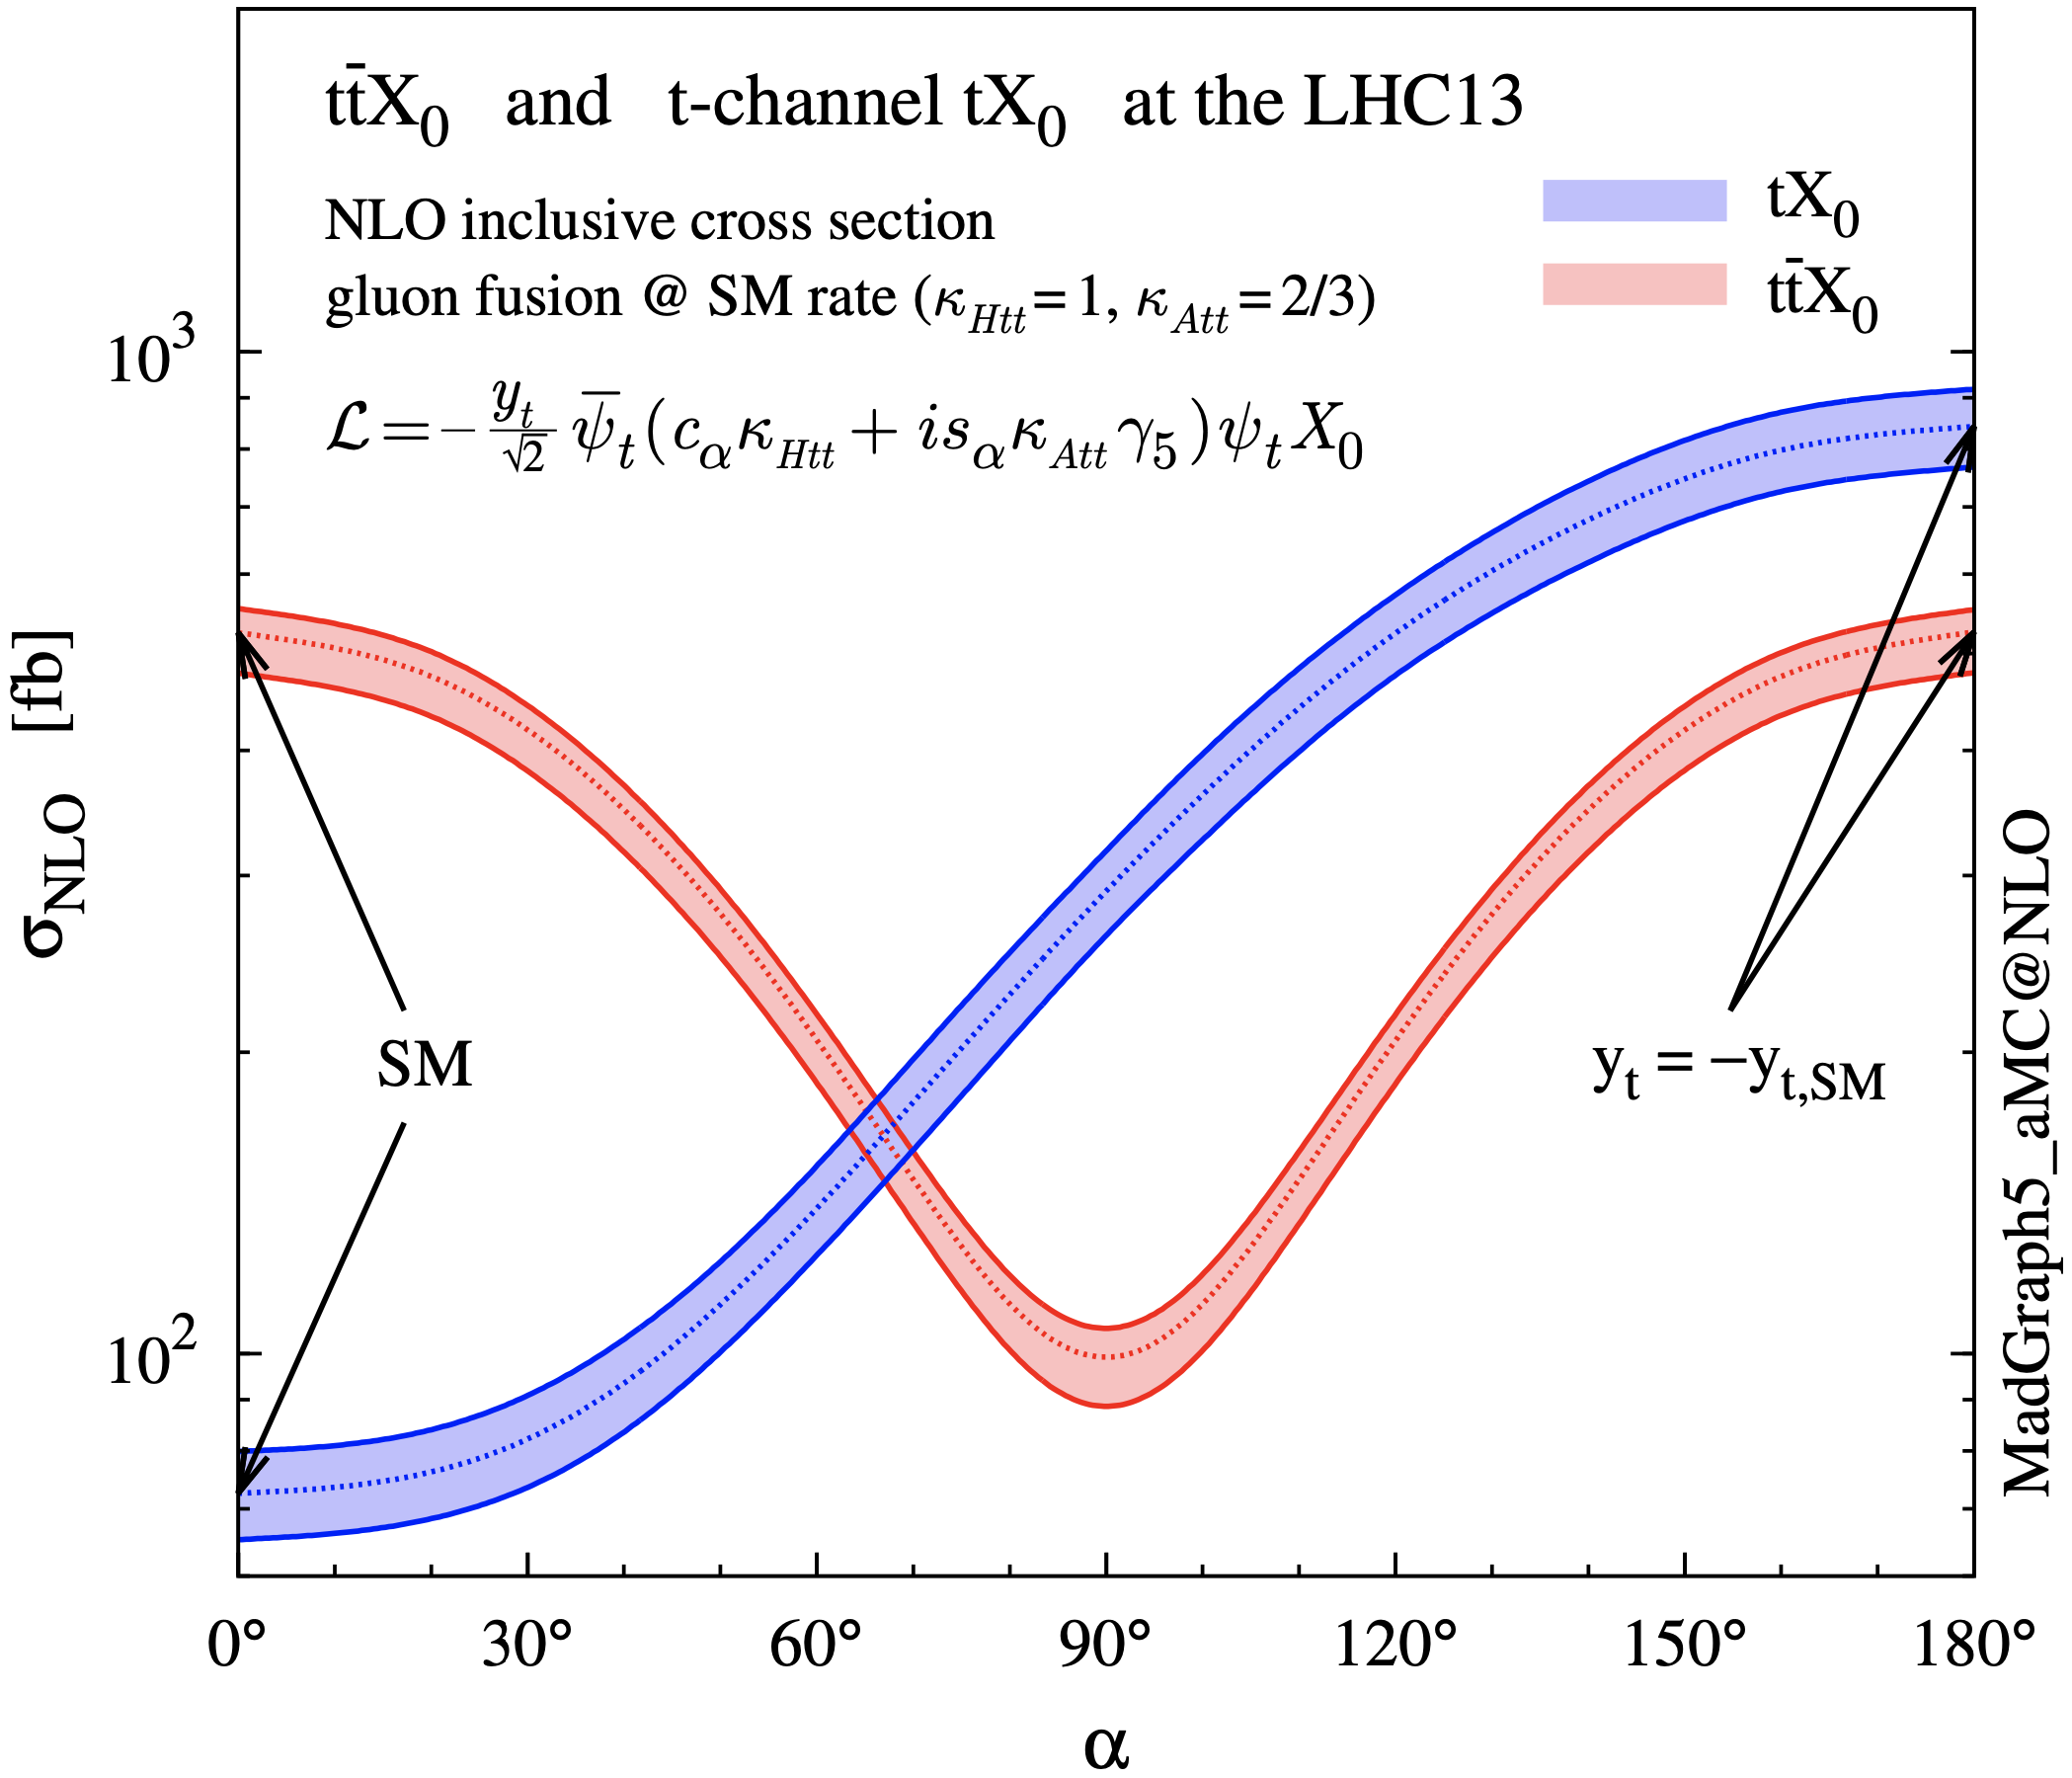
\includegraphics[width = 0.91\textwidth]{Chapter1/xsec_vs_yt_tH_ttH}
    \caption{Secció eficaç a NLO com a funció de l'angle de mescla de \CP 
    per a la producció $\Ptop X_{0}$ en el canal-$t$ i $\ttbar X_0$ a $\CM = 13$~TeV. 
    La particula $X_0$ representa un bosó de Higgs amb violació de \CP~\cite{Demartin:2015uha}.}
    \label{fig:Resum:xsec_vs_yt_tH_ttH}
\end{figure}

A l'hora d'observar la Figura~\ref{fig:Resum:xsec_vs_yt_tH_ttH}, la primera apreciació a tenir en compte és que 
la secció eficaç $\ttH$ és simètrica al voltant de $\alpha = \pi/2$. Això implica que mesurant 
$\sigma(\ttH)$ no seria possible discriminar entre escenaris de \CP parells i imparells. 
Per contra, per al procés \tH, no existeix eixa simetria i, llavors $\sigma(\tH)$ és sensible
a un possible acoblament que viole \CP.
Això es deu al fet que en l'SM, la producció \tHq on el \PHiggs es coupla amb el $\PW$ (Figura
\ref{fig:Resum:tHq:Feynman_LO} (b)) interfereix destructivament amb aquells en els quals el
\PH és radiat des del top (Figura~\ref{fig:Resum:tHq:Feynman_LO} (a)).




\FloatBarrier
%%%%%%%%%%
%   Experiment    %
%%%%%%%%%%
\section{L'experiment ATLAS de l'LHC al CERN}
\label{chap:resumen_val:Exp}
El Gran Col·lisionador d'Hadrons (LHC, per les seues sigles en anglés) és un accelerador de partícules que es troba 
al CERN (Centre Europeu per a la Recerca Nuclear o Laboratori Europeu de Física de Partícules Elementals), en 
Ginebra, Suïssa. Va ser dissenyat per a col·lisionar protons i ions pesats amb alta energia, permitint així als científics 
estudiar l'estructura subatòmica de la matèria i buscar noves partícules.

L'LHC és una màquina d'avantguarda que utilitza tecnologia avançada per accelerar partícules fins a velocitats 
properes a les de la llum abans de xocar-les entre si. El funcionament 
de l'LHC es basa en l'ús de camps magnètics i radiofreqüències per accelerar les partícules carregades.
A continuació, els feixos de partícules són dirigits per col·lissionar en els punts específics on es troben els detectors 
com ATLAS i CMS.
Aquestes col·lisions generen partícules secundàries que es 
registren mitjançant una xarxa de detectors situats en el seu interior. Les dades recopilades d'aquestes col·lisions 
es fan servir per a investigar la física de partícules. Amb energies de $\CM = 13$~TeV, l'LHC és l'accelerador de 
partícules més gran construït, la qual cosa constitueix una eina clau per a l'avanç de la ciència. 
Els quatre principals detectors que envolten l'LHC són: ATLAS, CMS, LHCb i ALICE. 
El primer d'aquests és l'experiment en el qual es desenvolupa el treball que es descriu 
en aquesta tesi doctoral. 




%\subsection{El gran col·lisionador d'hadrons}
%\label{chap:resumen_val:Exp:LHC}
% Take inspiration from https://www.benasque.org/2022imfp/talks_contr/084_IMFP2022_ARuiz.pdf
%El funcionament de l'LHC es basa en l'ús de camps magnètics i radiofreqüències per accelerar les partícules carregades. Les partícules, ja siguin protons o ions pesats, són injectades en anells d'acceleració que estan interconnectats per tubs a alta pressió anomenats feixos. Aquests feixos de partícules són accelerats fins a prop de la velocitat de la llum mitjançant camps magnètics generats per superconductors. A continuació, els feixos de partícules són dirigits a col·lidir en punts específics on es troben els detectors com ATLAS i CMS.

%%%%%%%
%   ATLAS  %
%%%%%%%
\subsection{El detector ATLAS}
\label{chap:resumen_val:Exp:ATLAS}
El detector ATLAS s'utilitza per mesurar les propietats de les partícules resultants de les col·lisions d'hadrons. 
ATLAS té una estructura cilíndrica i és un dels detectors de partícules més grans del món, amb aproximadament 
46 metres de llargària i 25 metres de diàmetre. Està compost per diversos components i subcomponents. 
Cada un d'aquests sistemes s'encarrega de registrar un tipus d'informació diferent. En ordre de dins cap a fora, 
ATLAS està format per:
\begin{itemize}
\item Detector intern (ID): Aquest component és el més proper al punt de col·lisió i té com a finalitat 
	rastrejar les trajectòries de les partícules carregades. L'ID està format per tres subcomponents:
	\begin{itemize}
	\item Detector de Píxels: És la part més interna de l'ID. El material de detecció és silici de $250\,\mu$m 
		de grossor. Cada mòdul conté 16 xips de lectura i altres components electrònics. La unitat mínima 
		de detecció és el píxel ($50\times400$~\textmu m), dels quals hi ha aproximadament 47000 per mòdul.
		La mida minúscula dels píxels està dissenyada per rastrejar de manera extremadament precisa prop del 
		punt d'interacció. El detector de píxels està compost per quatre capes dobles de tires de silici i té 6.3 milions de canals de 
		lectura i una àrea total de $61$~m$^{2}$.
		
	\item Rastrejador de Semiconductors (SCT):  Té un concepte i una funció similar al Detector de Píxels, 
		però amb tires llargues i estretes en lloc de petits píxels, fet que fa possible cobrir una àrea més extensa.
		Cada tira té una mida de $80$~\textmu m  $\times 12$~cm. El SCT és la part més crítica del detector intern per al 
		rastreig bàsic en el pla perpendicular al feix, ja que mesura partícules en una àrea molt més àmplia que el 
		Detector de Píxels.
		
	\item El Rastrejador de Radiació de Transició (TRT): Del l'anglés \textit{Transition Radiation Tracker}, és un 
		rastrejador de tubs de deriva\footnote{Straw chamber en anglés, es tracta d'un tub llarg amb un fil al centre i un
		gas que s'ionitza quan una partícula el travessa.}. Cada tub te un diàmetre 
		de $4$~mm, una longitud de fins a $144$~cm i està ple d'una mescla de gasos (principalment Xenó).
	\end{itemize}
	
\item Imant solenoidal: És un imant superconductor que envolta l'ID i genera un intens camp magnètic per desviar
	la trajectòria de les partícules carregades.
	
\item Calorímetre electromagnètic (ECAL): Aquest component té com a funció principal 
	mesurar l'energia de les partícules que interactuen electromagnèticament, com els 
	fotons i els electrons. Està format per capes de cristalls d'escintil·lació que generen 
	senyals de llum quan les partícules interactuen amb ells.
	
\item Calorímetre hadrònic (HCAL): A diferència de l'ECAL, aquest calorímetre està 
	dissenyat per mesurar l'energia de les partícules hadròniques, com els pions i 
	els protons. Està compost per capes de material dens que interactuen amb 
	les partícules, generant una cascada de partícules secundàries que 
	són detectades i mesurades.
	
\item Espectròmetre de muons (MS): Aquest component està dissenyat per mesurar i rastrejar 
	els muons, que tenen una gran capacitat de penetració. L'MS utilitza diferents tecnologies 
	de detectors per identificar i mesurar les trajectòries i les energies dels muons.
\end{itemize}




%%%%%%%
%   ATLAS  %
%%%%%%%
\subsection{Alineament del detector intern d’ATLAS}
\label{chap:resumen_val:Exp:Alignment}
Determinar amb precisió la trajectòria d'una partícula dins del detector
és una tarea determinant per poder reconstruir diversos observables físics. 
D'una banda la reconstrucció de les trajectores permet identificar quines partícules 
carregades han estat produïdes en una col·lisió. D'altra, la trajectòria 
d'una partícula carregada en un camp magnètic proporciona informació sobre 
la seua quantitat de moviment $\overrightarrow{p}$.
%Com es veu en la Secció~\ref{chap:resumen_val:Dades_i_Reco}, tot açó  
%permiteix obtindre infromació fonamental blablabla

La part del detector que s'encarrega de reconstruir les trajectories és l'ID.
Quan les partícules carregades travessen el detector, deixen dipòsits d'energia a 
cada subdetector (píxel), que permeten la reconstrucció de la trajectòria de la partícula. 
Amb més de 2 metres d'altura i 6 metres de longitud, l'AIDr té una precisió de mesura 
de posició millor que una centèsima de mil·límetre.  Per aconseguir aquesta precisió, 
el detector ha d'estar alineat amb una precisió igual o millor.

Un coneixement detallat de la geometria de l'ID és crucial per a una reconstrucció precisa.
La posició i forma dels subdetectors no són estacionàries sino que canvien amb el temps.
Els elements del detector poden 
desplaçar-se a causa de fluctuacions de temperatura o de canvis en el camp magnètic. 
Per tindre en compte aquests moviments, es realitza amb regularitat l'alineament
del ID i es determina la geometria real de cada element actiu del subdetector.
Aquest alineament s'ha de dur a terme mitjançant mètodes indirectes, perquè el detector 
és inaccessible durant el funcionament de l'LHC.

L'algoritme d'alineament d'ATLAS està basat en la comparació dels punts d'impacte registrats 
amb la trajectòria reconstruïda de les partícules. Si la posició d'un subdetector és correctament 
coneguda, les diferències residuals s'equilibraran. En cas contrari, els residuals mostraran un 
desviament sistemàtic, indicant el desalineament d'un subdetector.   
Aquest és un procés iteratiu que  segueix l'estructura jeràrquica de l'ID, primer alineant les grans 
estructures físiques i després els elements individuals del subdetector.
La Figura~\ref{fig:Resum:Alignment:Residual} mostra les diferències residuals produïdes
pel desalineament de l'ID.

\begin{figure}[h]
	\centering
	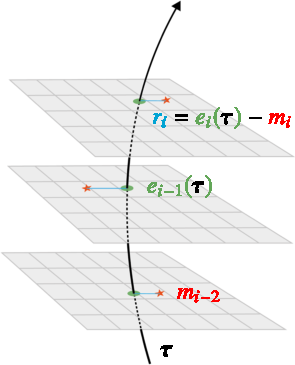
\includegraphics[width = 0.5\textwidth]{Chapter2/Alignment_residual}
	\caption{La línia negra és la trajectòria reconstruida de la partícula que creua l'ID.
	L'estrella roja representa la mesura en cada capa del detector i les diferències residuals
	estan representats per la linea blava~\cite{ATLAS:2020ixw}.  }
\label{fig:Resum:Alignment:Residual}
\end{figure}

\subsubsection{Visor Web de Monitoratge de l'Alineament de l'ID}
Atés que qualsevol desalineació dels diferents elements de l'ID deteriorarà la qualitat de la 
reconstrucció de trajectòries i objectes és obligatori un seguiment constant de l'alineació.
Durant la producció d'aquesta tesi, he contribuït a l'alineament de l'ID a través del desenvolupament 
del sofware de monitoratge dels resultats de l'alineament de l'ID d’ATLAS descrits amunt. 

El visor web de Monitoratge de l'alineació de l'ID és una aplicació destinada a la monitoratge dels resultats 
de l'alineament basats en trajectòries aconseguits en el bucle de calibració per a l'ID. Ajuda a avaluar les 
correccions d'alineació calculades així com moltes distribucions gràfiques directament relacionades amb el 
rendiment (per exemple, els residus del detector).  A la Figura~\ref{fig:Resum:Alignment:WebDisplay} es
mostra la pàgina principal del visor web que he desenvolupat. 

\begin{figure}[h]
	\centering
  	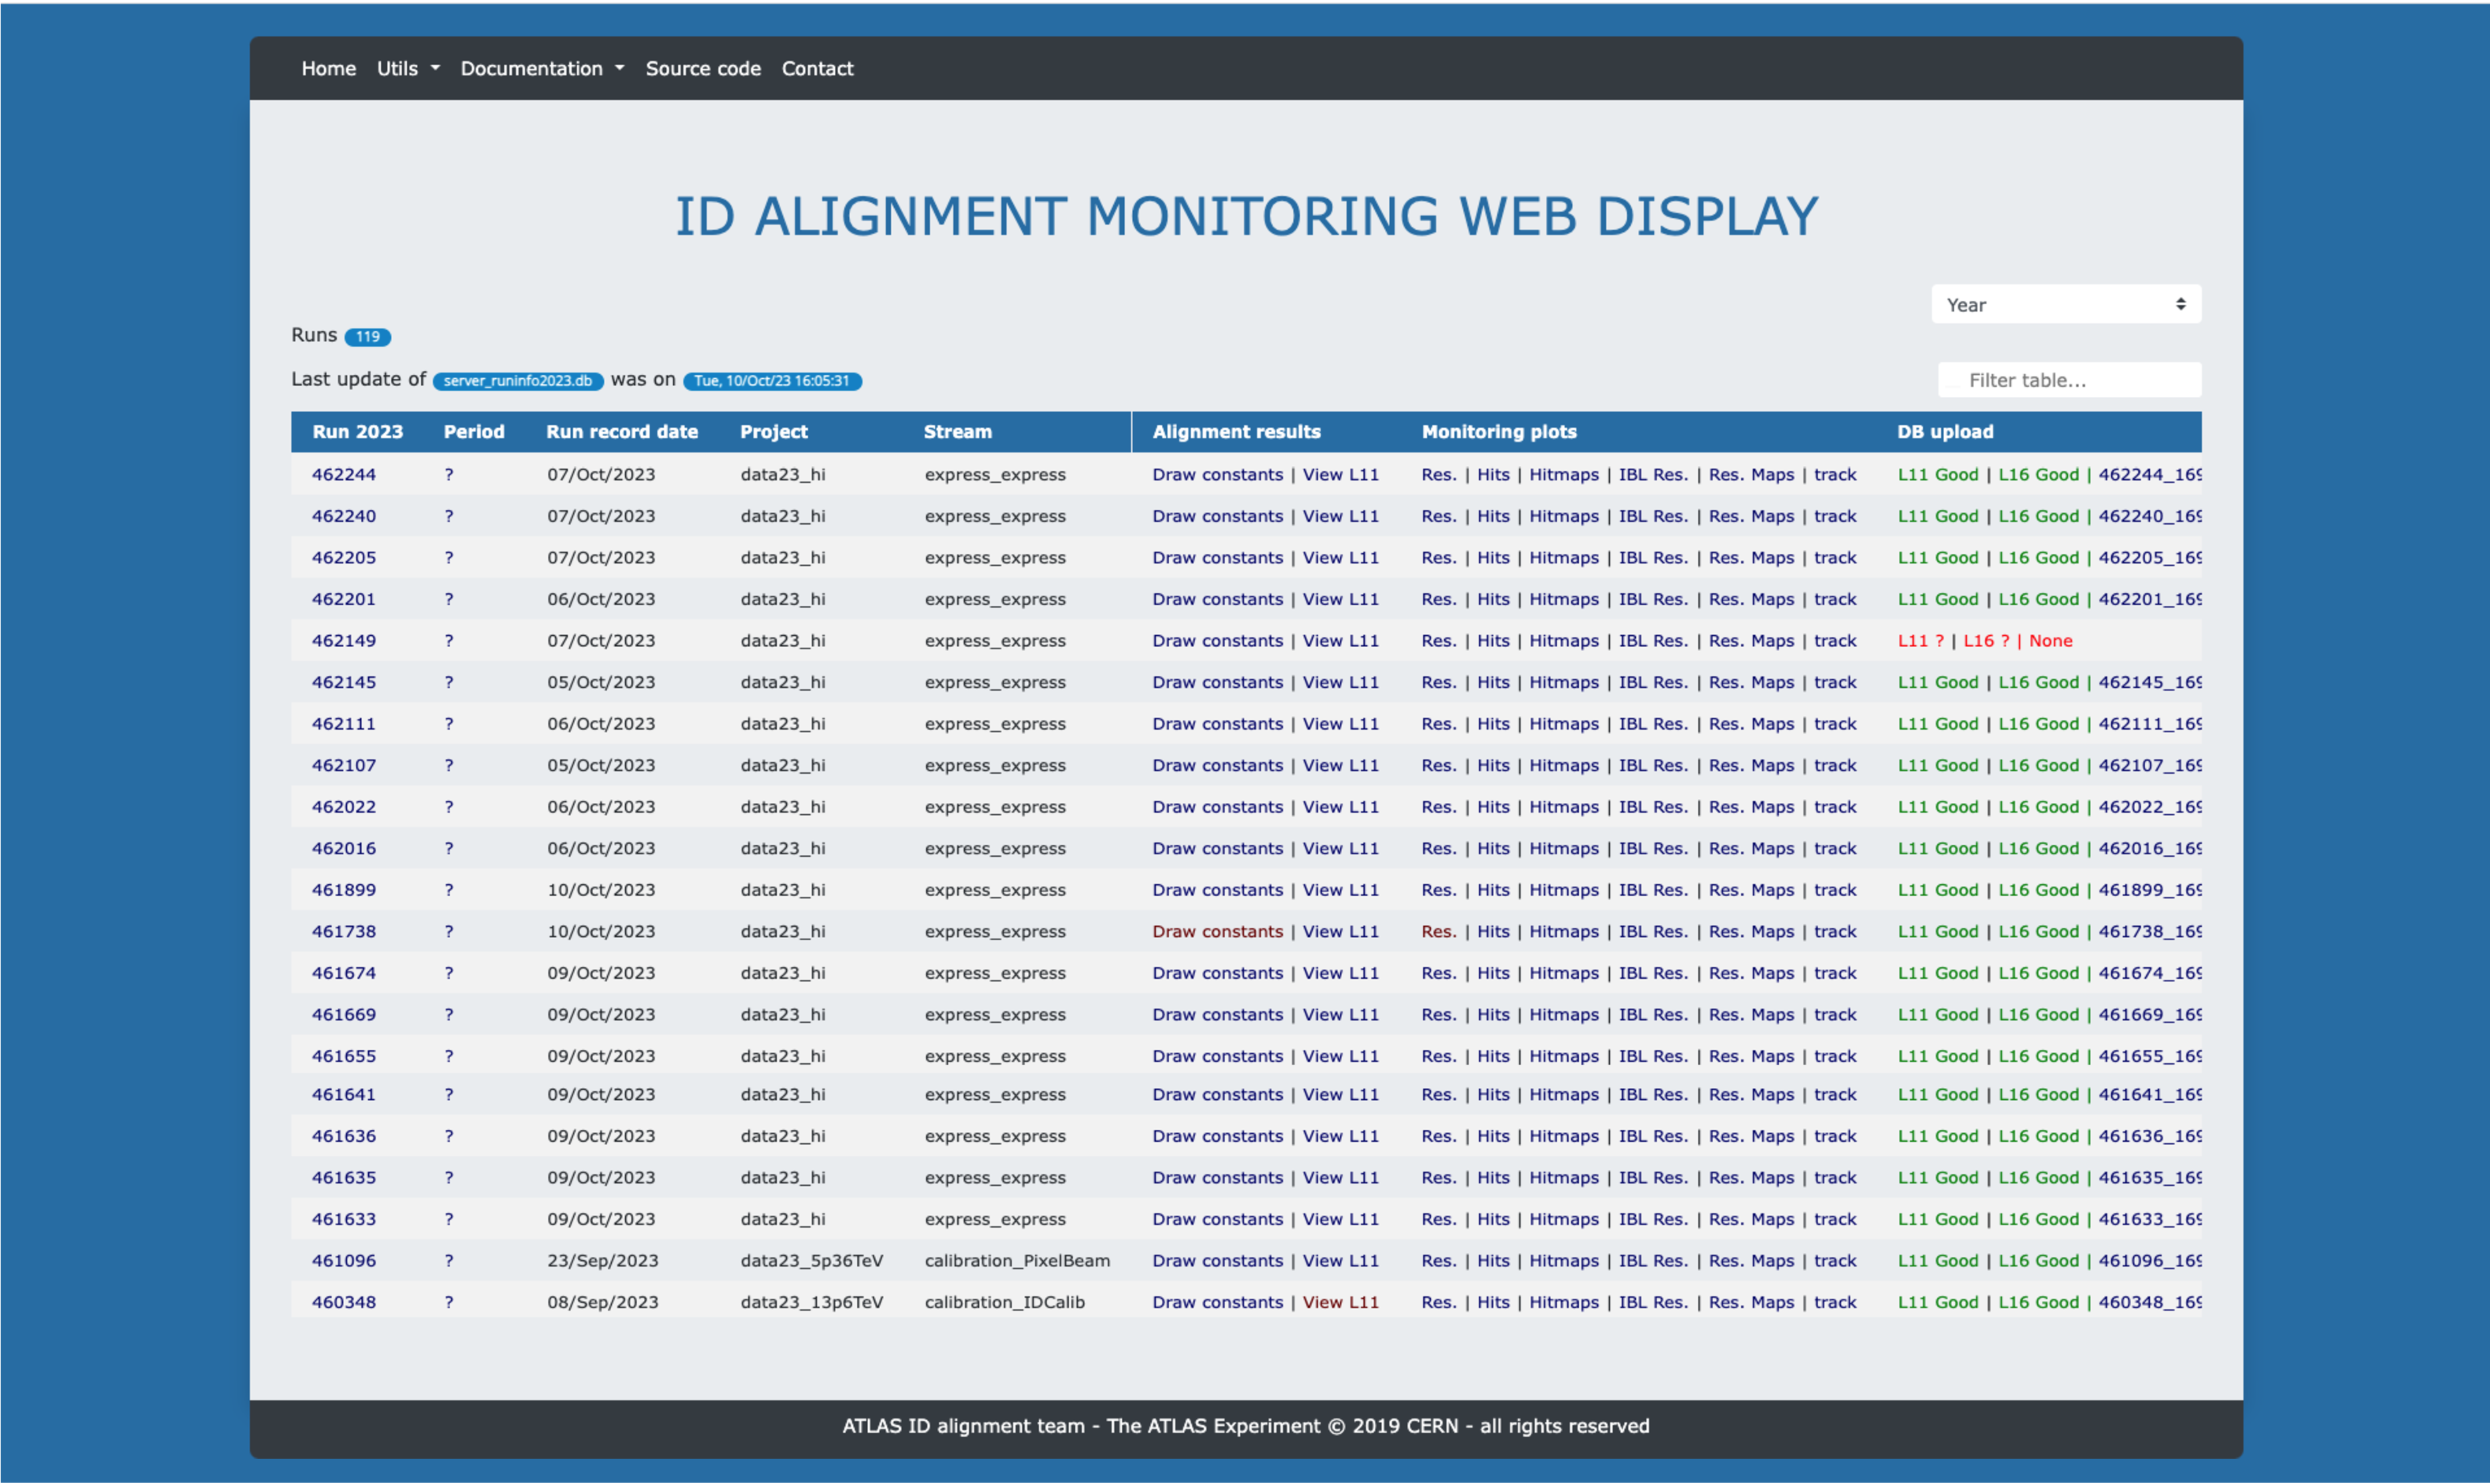
\includegraphics[width=0.9\columnwidth]{Chapter2/WebDisplay_Bueno}
	\caption{Pàgina principal del Visor Web de Monitoratge de l'Alineació de l'ID.}
	\label{fig:Resum:Alignment:WebDisplay} 	
\end{figure}


Les meues responsabilitats incloïen el desenvolupament i implementació del codi tant per a la part client 
(frontend) com per a la part del servidor (backend) per al Visor Web de Monitoratge de l'Alineació de l'ID.
S'han realitzat millores significatives en aquesta eina, incloent-hi la integració amb la configuració estàndard 
d'Athena, la conformitat amb els estàndards d'estil d'ATLAS, millors en l'eficiència d'execució i actualitzacions
dinàmiques, així com una major interactivitat del frontend.
A més, s'ha optimitzat el codi per a eliminar redundàncies i s'ha millorat la interfície d'usuari per a facilitar 
l'accés i la gestió de les dades.

Aquestes millores no només augmenten la velocitat d'execució de l'aplicació, sinó que també proporcionen 
accés a més informació i permeten gestionar i accedir fàcilment a les dades desitjades. El Visor Web de 
Monitoratge de l'Alineació de l'ID que he desenvolupat s'està utilitzant activament pels membres de la 
col·laboració ATLAS per a monitorar l'alineació de l'ID durant la Run 3 així com en el reprocessament de les 
dades de la Run 2. Això ha simplificat significativament el monitoratge de l'alineació, fent la tasca més eficient 
i fàcil de fer servir.


%\section{Mesura de la polarització del quark top al canal-\textit{t}}
%Mesura d’observables sensibles a la polarització del quark top
%\subsection{Selecció d’esdeveniments}
%\subsection{Estimació del fons}
%\subsection{Fonts d’incertesa}
%\subsection{Resultats}

\FloatBarrier
%%%%%%%%%%%%%%%%%%%%%%%%%%%%%%%%
%   Recolecció de dades, simulació i recontrucció d'obejectes  %
%%%%%%%%%%%%%%%%%%%%%%%%%%%%%%%%%
\section{Recol·lecció de dades, simulació i reconstrucció d'objectes}
\label{chap:resumen_val:Dades_i_Reco}
\subsection{Simulació i adquisició d'esdeveniments en ATLAS}
La simulació i l'adquisició de dades són també una part fonamental de l'anàlisi, ja que 
és amb elles amb les quals es realitzarà posteriorment l'estudi del procés \tHq.

Per l'anàlisi descrita en aquesta tesi, les dades utilitzades són les recollides pel detector ATLAS 
durant el Run 2, és a dir, del 2015 al 2018. Les dades van ser produïdes durant col·lisions $\Pproton \Pproton$  
a l'LHC amb una freqüència de $25$~ns a $\CM=13$~TeV. La lluminositat total integrada aconseguida 
durant aquest període va ser de $140$~fb$^{–1}$, amb un error que varia entre el 2,0\% i el 2,4\%.

La simulació d'esdeveniments, també coneguda com a simulació Monte Carlo (MC), es divideix en 
diverses etapes que abasten des del càlcul de la secció eficaç a escala de partons (quarks i gluons) 
fins a les cascades de partons i els efectes no pertorbatius del procés, i finalment, la simulació de la 
interacció de les partícules pel detector i el senyal elèctrica d'aquest. Els diferents passos 
d'una col·lisió de $\Pproton\Pproton$ que cal tenir en compte es mostren de forma esquemàtica 
a la Figura~\ref{fig:Resum:ttHSimulated}.


 \begin{figure}{t}
    \centering
    \includegraphics[width = \textwidth]{Chapter3/Generator_ttH}
    \caption{Esquema d'una col·lisió $\Pproton \Pproton$ per a produir un esdeveniment \ttH.  
    El gran punt roig representa la interacció forta principal, seguida de la desintegració del bosó Higgs i els dos quarks top, 
    representats pels tres punts rojos més petits.  Els punts blaus indiquen els partons en el seu estat inicial. Els processos de dispersió forta secundaris es mostren en violeta. Finalment, es mostra el procés d'hadronització (en verd clar) i els estats finals hadrònics (en verd). A més, apareixen unes línies grogues que representen la radiació de fotons. }
    \label{fig:Resum:ttHSimulated}
\end{figure}

La simulació de MC inclou diversos processos físics: la dispersió de QCD, també coneguda 
com la creació dels elements de matriu; la cascada de partons, l'hadronització, els processos 
de dispersió de QCD secundaris, desitegracions i el \text{pile-up}. Cada un d'aquests processos 
es simula de forma independent i utilitza diferent informació d'entrada.

Hi ha diversos programes al mercat per realitzar una o diverses parts de la simulació. 
Els utilitzats en algunes de les simulacions a l'anàlisi inclosa en aquesta tesi són: 
\POWHEGBOX, \MGNLO, \SHERPA, \PYTHIA  i \HERWIG. Alguns d'ells han 
estat utilitzats per la simulació nominal d'un procés, mentre que d'altres s'han
utilitzat per obtenir l'error derivat de l'ús d'un programa o l'altre.

L'últim pas de la simulació d'esdeveniments és la simulació del pas de les partícules pel detector, 
la qual cosa es realitza a través d'Athena~\cite{Duckeck:2005rb, Mato:1998gfa}, 
un software específic de la col·laboració ATLAS, utilitzant \GEANT~\cite{GEANT4:2002zbu}.
% Full and detailed geometry :: Full simulation
% Just calorimeter :: Fast simulation


Les diferents combinacions de generadors de MC utilitzades tant per 
al procés de senyal com per a tots els fons considerats es mostren 
en la Taula~\ref{tab:Resum:Data_and_MC:MCsummary}. La influència a l'anàlisi
dels processos llistats a la Taula~\ref{tab:Resum:Data_and_MC:MCsummary}
no és uniforme.

\begin{table}[!htbp]  
  \begin{adjustbox}{max width=0.99\textwidth}
    \begin{tabular}{llllll}
      \toprule
      Procés & Generador de MC & Ordre (esquema) & Joc de PDF & Cascada de partons & Joc de PDF \\
      \midrule
      \multicolumn{6}{c}{Signal} \\
      \midrule
      \tHq & \MGNLO[2.6.2] & NLO (4FS) & \NNPDF[3.0nlo] nf4 & \PYTHIA[8.230] & \NNPDF[2.3lo] (A14 tune) \\
      \midrule
      \multicolumn{6}{c}{Fons} \\
      \midrule
      \ttbar & \POWHEGBOX[v2] & NLO (5FS) & \NNPDF[3.0nlo] & \PYTHIA[8.230] & \NNPDF[2.3lo] (A14 tune) \\
      \(V\)+jets & \SHERPA[2.2.1] & NLO+LO & \NNPDF[3.0nnlo] & - & - \\
      \Diboson & \SHERPA[2.2.1-2] & NLO+LO & \NNPDF[3.0nnlo] & - & -\\
      \Triboson & \SHERPA[2.2.2] & NLO+LO & \NNPDF[3.0nnlo] & - & - \\
      \ttZ & \MGNLO[2.3.3] & NLO & \NNPDF[3.0nlo] & \PYTHIA[8.210] & \NNPDF[2.3lo] (A14 tune) \\
      \ttW & \SHERPA[2.2.10] & NLO & \NNPDF[3.0nnlo] & - & - \\
      %\ttV & \MGNLO[2.3.3] & NLO & \NNPDF[3.0nlo] & \PYTHIA[8.210] & \NNPDF[2.3lo] (A14 tune) \\
      \ttH & \POWHEGBOX[v2] & NLO (5FS) & \NNPDF[3.0nlo] & \PYTHIA[8.230] & \NNPDF[2.3lo] (A14 tune) \\
      \(t\)-channel & \POWHEGBOX[v2]  & NLO (4FS) & \NNPDF[3.0nlo] nf4 & \PYTHIA[8.230] & \NNPDF[2.3lo] (A14 tune) \\
      \Wt & \POWHEGBOX[v2] & NLO (5FS, DR) & \NNPDF[3.0nlo] & \PYTHIA[8.230] & \NNPDF[2.3lo] (A14 tune) \\
      \(s\)-channel & \POWHEGBOX[v2] & NLO & \NNPDF[3.0nlo] & \PYTHIA[8.230] & \NNPDF[2.3lo] (A14 tune) \\
      \tZq & \MGNLO[2.3.3] & NLO & \NNPDF[3.0nlo] & \PYTHIA[8.230] & \NNPDF[2.3lo] (A14 tune) \\
      \tHW{} & \MGNLO[2.8.1] & NLO (5FS, DR) & \NNPDF[3.0nlo] & \PYTHIA[8.245p3] & \NNPDF[2.3lo] (A14 tune) \\
      \tWZ & \MGNLO[2.3.3] & NLO & \NNPDF[3.0nlo] & \PYTHIA[8.212] & \NNPDF[2.3lo] (A14 tune) \\
      \ttt & \MGNLO[2.2.2] & NLO & \NNPDF[3.1nlo] & \PYTHIA[8.186] & \NNPDF[2.3lo] (A14 tune) \\
      \tttt & \MGNLO[2.3.3] & NLO & \NNPDF[3.1nlo] & \PYTHIA[8.230] & \NNPDF[2.3lo] (A14 tune) \\
      \ggH & \POWHEGBOX[v2] & NLO & \CT[10] & \PYTHIA[8.210] & \CTEQ[6L1] (\AZNLO tune) \\
      \qqH & \POWHEGBOX[v1] & NLO & \CT[10] & \PYTHIA[8.186] & \CTEQ[6L1] (\AZNLO tune) \\
      \WH & \PYTHIA[8.186] & LO & \NNPDF[2.3lo] & - & - \\
      \ZH & \PYTHIA[8.186] & LO & \NNPDF[2.3lo] & - & - \\
      \bottomrule
    \end{tabular}
  \end{adjustbox}
  \caption{Resum de les mostres d'esdeveniments simulats de senyal i fons bàsics 
  utilitzades en els anàlisis de \tHq.}
  \label{tab:Resum:Data_and_MC:MCsummary}
\end{table}




\subsection{Identificació i reconstrucció d'objectes en ATLAS}
Els senyals proporcionats pels diferents components del detector ATLAS són
transformats en objectes físics reconstruïts per poder emprar-los en les diferents anàlisis.
Un objecte físic fa referència a una partícula o entitat similar a una partícula reconstruïda detectada dins d'ATLAS
com a conseqüència d'una col·lisió de partícules.
Els principals objectes físics que es detecten i reconstrueixen per a aquesta tesi són:

\begin{itemize}
\item \textbf{Electrons}: 	Reconstruïts utilitzant els dipòsits d'energia en el ECAL, coincidents amb trajectòries a l'ID.
					Sense una bona resolució a l'hora de reconstruir les traces, seria imposible 
					identificar i reconstruir partícules carregades~\cite{ATLAS:2019qmc}. 
					Per això, un correcte alineament del
					ID es fonamental, tal com es descriu en la Secció~\ref{chap:resumen_val:Exp:Alignment}.
					A aquesta análisi, les condicions fetes servir per etiquetar un objecte com a electró són les
					recomanades pel \textit{Combined Performance group} i consisteixen a tenir un \pT superior
					a 10~GeV, estar dins de l'interval de pseudorapidesa de $|\eta^\mathrm{clust}| < 2.47$, i 
					superar el nivell d'identificació estricte. S'apliquen condicions sobre l'aïllament per a reduir
					l'impacte dels electrons que no provenen del procés principal (electrons \textit{non-prompt}).  
				
\item \textbf{Muons}:		Es reconstrueixen associant traces en la cambra de muons amb traces en l'ID,
					complementant aquesta informació amb el senyal dels calorímetres~\cite{ATLAS:2016lqx}.
					De nou, es veu la necessitat d'un bon alineament a l'ID. 
					Al nostre anàlisi es requereix que els muons tinguen $\pt > 7$GeV, $|\eta| < 2.5$,
					i que passen un criteri d'identificació mitjà %~\cite{MCPRecommendations}.
					Igual que amb els electrons, es demanda una estricte aïllament dels candidats a muons.
					% Dins d'ATLAS hi ha diverses formes de reconstruir els muons. La que es du a terme a
					% aquesta anàlisi requerix les condicions descrites a la 
					% Taula~\ref{tab:Resum:ObjectDefReco:Electrons_Muons}.
					

\item \textbf{Leptons tau}:	El leptó \Ptau, amb una massa de $1.78$~GeV, és l'únic leptó 
					prou massiu per desintegrar-se en hadrons. En aproximadament un 
					terç dels casos, els leptons \Ptau es desintegren de manera leptònica (\taulep) en 
					un muó o un electró amb dos neutrins. Els \taulep no es reconstrueixen com a tal,
					sinó que directament s'identifiquen els muons i electrons. En 
					els casos restants, els tau leptons es desintegren de manera hadrònica, 
					en una combinació de mesons carregats i neutres amb un \Pnut. 
					Els leptons \Ptau que es desintegren hadrònicament, coneguts com 
					a \tauhad, es reconstrueixen i identifiquen fent servir una xarxa neuronal recurrent.
					A més, una BDT per a vetar electrons es utilitzada.
					
					Per a acceptar un
					objecte físic com a \tauhad es precís que aquest tinga associades una o tres 
					traces i que es trobe en espai definit $|\eta^\mathrm{clust}| < 2.5$ excluint 
					$1.37 < |\eta^\mathrm{clust}| < 1.52$.  També es requereix un \pT mínim
					de $20$~GeV. Una Xarxa Neuronal Recurrent (RNN) és emprada per
					realitzar l'identificació.

\item \textbf{Jets}: 	Formats per la conglomeració de dipòsits d'energia al calorímetre hadrònic, 
				que sorgeixen de l'hadronització de quarks i gluons produïts en les col·lisions.
				Els jets són feixos de partícules estretament agrupades i altament col·limades 
				que es mouen en la mateixa direcció, seguint la direcció original del quark o gluó original.
				Aquests objectes es reconstrueixen a partir dels dipòsits d’energia en els calorímetres i 
				les traces de l'ID.  Aquesta informació és combinada utilitzant l’algoritme \Akt 
				\cite{Cacciari:2008gp}.  
				
				Per a aquesta anàlisi, s'aplica el requisit de que el \pT siga superior a $20$~GeV
				i es trobe contigunt en $|\eta|<4.5$. 
				
\item \textbf{Jets-\Pbottom}:	Jets que provenen de l'hadronització de quarks bottom.
						La seua identificació es fa mitjançant diferents algoritmes 
						que exploten els seus trets característics, com els seus paràmetres 
						d’impacte, la presència de vèrtexs secundaris o la seua topologia de 
						desintegració. Particularment, l'algoritme \texttt{DL1r} és utilitzat en
						aquesta anàlisi. Aquest mètode està basat en una xarxa neural recurrent
						\cite{ATL-PHYS-PUB-2017-003}. 
						També cal que es satisfaça que  $\pt > 20$~GeV, $|\eta^\mathrm{clust}| < 2.5$.
						
\item \textbf{Energía transversa mancant}:  També coneguda com a moment transvers de falta, 
						és una quantitat important que representa el desequilibri del moment 
						transvers en un esdeveniment. La \MET es deu a partícules no detectades,
						 que en el cas de la nostra anàlisi són els neutrins.

\end{itemize}

\begin{comment}
\begin{table}[!htbp]
\centering
  \begin{adjustbox}{max width=0.95\textwidth}
  \begin{tabular}{ l|l|l }
    \toprule
    & \multicolumn{1}{c|}{Electró} & \multicolumn{1}{c}{Muó} \\
    \midrule
    Identificatió   & \multicolumn{1}{c|}{\texttt{tightLH}} &  \multicolumn{1}{c}{\texttt{medium}}\\
    Acceptància       & $\pt > 10$~GeV, $|\eta^\mathrm{clust}| < 2.47$  & $\pt > 10$~GeV, $\abseta < 2.5$ \\
                     &  except $1.37 < |\eta^\mathrm{clust}| < 1.52$          & \\
    Paràmetre d'imapcte & $|\dzero/\sigma(\dzero)| < 5.0$                   & $|\dzero/\sigma(\dzero)| < 3.0$ \\
                     & $|\zzsth| < 0.5$~mm                      & $|\zzsth| < 0.5$~mm \\
    Aïllament        & \texttt{PLImprovedTight}  & \texttt{PLImprovedTight} \\
    Adicionals & ECIDS, $e/\gam$ ambiguity-cuts &  \\
    \bottomrule
  \end{tabular}
   \end{adjustbox}
  \caption{Definicions per seleccionar electrons i muons.\pablo{¿Explicar estas los parámetros de la tabla?.}}
   \label{tab:Resum:ObjectDefReco:Electrons_Muons}
\end{table}



\begin{table}[!htbp]
\centering
\begin{adjustbox}{max width=0.95\textwidth}
\begin{tabular}{l|l}
\toprule
			& \multicolumn{1}{c}{\tauhad} \\
\midrule
Acceptancia     	& $\pt > 20$~GeV, $|\eta^\mathrm{clust}| < 2.5$   \\
			&  excepte $1.37 < |\eta^\mathrm{clust}| < 1.52$         \\
Nombre de traces & 1 or 3\\
Identificació 	& \texttt{RNN Medium (Loose)} \\
Veto per electrons  & \texttt{electró BDT Loose (Loose)}   \\
\bottomrule
\end{tabular}
 \end{adjustbox}
\caption{Condicions per considerar un objecte com a \tauhad.}
\label{tab:Resum:ObjectDefReco:Tau}
\end{table}
\end{comment}




\FloatBarrier
%%%%%%%%%%%%%%%
%   Mesura de process tHq  %
%%%%%%%%%%%%%%%
\section{Recerca de processos \tHq amb un estat final \dileptau}
\label{chap:resumen_val:tHq}
L'objectiu principal d'aquesta anàlisi és establir límits en la secció eficaç de producció del procés \tHq. 
La producció de \tHq s'analitza a través de sis canals ortogonals optimitzats de manera independent 
(presentats a la Taula~\ref{tab:ResumChaptH:tHqChannels}),
centrant-se aquesta tesi en l'estat final amb dos leptons lleugers (\emu) i un leptó tau que es desintegra hadrònic (\tauhad).
El canal \dileptau es divideix en dues subcategories depenent
del signe relatiu de la càrrega elèctrica mostrada pels dos leptons lleugers carregats: El canal \dilepOStau si la càrrega és oposada
i el \dilepSStau si tenen la mateixa càrrega. Els diagrames de Feynman corresponent a aquestos dos modes de producció es
presenten a la Figure~\ref{fig:resum:ChaptH:dileptauFeynmanDiagram}. 


Per als canals amb estats finals multileptònics, l'analisi considera tres modes de desintegració
del bosó de Higgs: $\PHiggs \rightarrow \PWplus\PWminus$,  
$\PHiggs \rightarrow  \Ptauon \APtauon$ y $\PHiggs \rightarrow  \PZ\PZ$. 
La Taula~\ref{tab:Resum:ChaptH:tHqChannelsYields} mostra l'importància de 
cada un dels modes de desintegració dins de cada canal de cerca \tHq. 
Es important notar que, en conjunt, aquestos tres modes
representen únicament el 21\% del total de la fracció de dessintegració del bosó de Higgs
tal i com s'explica a la Secciò~\ref{sec:resum:FisicaHiggs}.


\begin{table}[]
\centering
\begin{tabular}{l|c|c|c}
\toprule
 \#				& 0 \tauhad       & 1 \tauhad               	& 2 \tauhad                \\ \midrule
$1\ell$ (\Pe / \Pmu) 	& \begin{tabular}[c]{@{}c@{}}\tHq(\bbbar) \\  $1\Plepton$\end{tabular}&              & \begin{tabular}[c]{@{}c@{}}\tHq$(\PW\PW/\PZ\PZ/\Ptau\Ptau)$ \\ \lepditau \end{tabular}	\\
$2\ell$ 	(\Pe / \Pmu) 	& \begin{tabular}[c]{@{}c@{}}\tHq($\PW\PW/\PZ\PZ/\Ptau\Ptau$)  \\  \dilepSS\end{tabular} & \begin{tabular}[c]{@{}c@{}}\tHq($\PW\PW/\PZ\PZ/\Ptau\Ptau$) \\ \dileptau \end{tabular}&   	\\
$3\ell$ 	(\Pe / \Pmu) 	& \begin{tabular}[c]{@{}c@{}}\tHq($\PW\PW/\PZ\PZ/\Ptau\Ptau$) \\ \trilep 	\end{tabular}	&               &               	\\
\bottomrule
\end{tabular}
\caption{Diferents canals per a la producció de \tHq segons la presència de leptons de sabor lleuger i
taus que es desintegren hadrònicament en l'estat final. 
Els requisits de multiplicitat sobre els objectes d'estat final,
asseguren l'ortogonalitat entre canals per a una futura combinació.}
\label{tab:ResumChaptH:tHqChannels}
\end{table}



\begin{table}[]
\centering
\begin{tabular}{l|lll}
\toprule
Canal  	& \Htautau & \HWW	& \HZZ \\
\midrule
\dileptau 	& 63      	& 32  	& 5   \\
\lepditau 	& 96      	& 3   		& 1   \\
\dilepSS  	& 17      	& 80  	& 3   \\
\trilep   	& 14      	& 69  	& 17 \\
\bottomrule	
\end{tabular}
\caption{La probabilitat percentual dels modes de desintegració del bosó de Higgs
dins dels diferents canals multipleptònics ha sigut calculada utilitzant les fraccions de desintegració.}
\label{tab:Resum:ChaptH:tHqChannelsYields}
\end{table}

 
 
 \begin{figure}[htbp!]
  \centering  
  \begin{subfigure}[b]{0.45\textwidth}
    \centering
    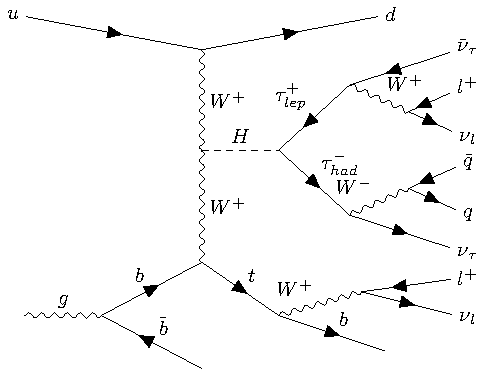
\includegraphics[width=\textwidth]{Feynman_diagrams/Feynman_DileptauGeneralRepresentative_dileptau_SS}
    \caption{\dilepSStau}
    \label{fig:tHq:Resum:diltauFeynmanDiagram:SS}
  \end{subfigure}
  \hfill
  \begin{subfigure}[b]{0.45\textwidth}
    \centering
    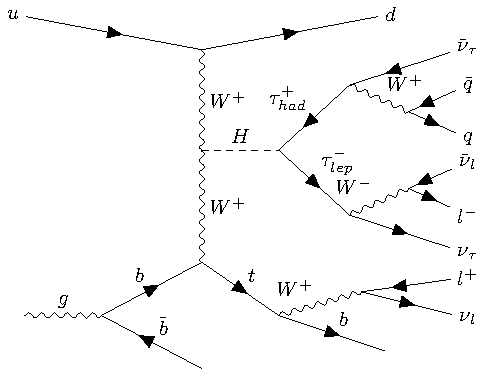
\includegraphics[width=\textwidth]{Feynman_diagrams/Feynman_DileptauGeneralRepresentative_dileptau_OS}
    \caption{\dilepOStau}
    \label{fig:tHq:Resum:diltauFeynmanDiagram:OS}
  \end{subfigure}
  \caption{Diagrames a ordre dominant per a la producció \tHq (\dileptau) al canal de desintegració $\PHiggs \rightarrow \tauhad \taulep$.
Es pot apreciar que el dos leptons lleugers al diagrama (a) tenen la mateixa càrrega elèctrica mentre que en (b) la càrrega és oposada.}
  \label{fig:resum:ChaptH:dileptauFeynmanDiagram}
\end{figure}



\subsection{Estudis sobre la senyal}
\label{chap:resumen_val:tHq:Senyal}
Per tal de poder separar els processos \tHq de els fons, cal comprendre les propietats
d'aquesta producció. D'aquesta manera podrem definir observables físics (comunament referits com variables)
que ens permeten discriminar el senyal per tal crear regions a l'espai de fases enriquides en processos \tHq,
tal com es fa en la Secció~\ref{chap:resumen_val:tHq:Seleccio}. El primer pas per fer açò és obtenir la informació del senyal a escala de partons. Després, utilitzant aquesta informació, l'origen del leptons lleugers (és a dir, si venen
de la desintegració del bosó de Higgs o de la del quark top) pot ser determinat. Finalment, açò pot ser emprat per
reconstruir les propietats cinemàtiques dels processos \tHq i, amb aquestes, definir variables.


\subsubsection{Validació de les simulacions a nivell de partons}
\label{chap:resumen_val:tHq:Senyal:truth}
%Tal com s'exposava en la Secció~\ref{chap:resumen_val:Dades_i_Reco}, l'informació
%a escala de partons és aquella a la qual encara no s'han tingut en compte els efectes de
%la interacció de les partícules amb el detector.

Dins de la col·laboració ATLAS, per tal de generar i administrar la informació a nivells de partons, el
paquet de software \texttt{TopPartons} és emprat. Una de les contribucions %~\cite{TopPartonsGitLab}
d'aquesta tesi ha sigut el desenvolupament dels codis necessaris per a incloure en aquest paquet els processos \tHq.
Per tal de validar que el programa elaborat funciona correctament, s'han realitzat càlculs teòrics per comparar-los amb el resultat
del paquet.

El paquet elaborat guarda a les NTuples\footnote{Una \textit{NTupla} es refereix a un format de dades utilitzat
per emmagatzemar i organitzar informació detallada sobre les col·lisions de partícules i les simulacions. 
Les nostres NTuples estan al format ROOT~\cite{Brun:1997pa}.}
la informació de totes les partícules que apareixen al diagrama de Feynman dels processos \tHq.
Aquesta informació consisteix en el PDG-ID\footnote{Un nombre que identifica la identitat de la partícula.}, \pT, $\eta$, $\phi$ i massa. Addicionalment, per als leptons $\tau$,
es guarda la informació sobre si aquests es desintegren lacònicament o hadrònicament.
Aquest desenvolupament es fet servir per tots els canals que participen en la cerca del procés \tHq.

Pel que fa als càlculs per validar \texttt{TopPartons}, aquests s'han fet combinant les fraccions de desintegracions
de totes les partícules involucrades a les cadenes de desintegració del quark top i el bosó Higgs. Després s'han estudiat
totes les combinacions d'aquestes partícules que podien generar els estats finals \dileptau. Gràcies a aquests càlculs podem
conéixer les contribucions de cada canal de desintegració a l'estat final i també determinar on es produeix el \tauhad.
Aquests resultats són recollits a la Taula~\ref{tab:ResumChaptH:TruthSummary}.


\begin{table}[h]
\centering
\begin{adjustbox}{max width=0.95\textwidth}
\begin{tabular}{l|ll|l}
\toprule
       \multicolumn{1}{c|}{Canal de} 	& \multicolumn{2}{c|}{Origin del \tauhad} &    \multirow{2}{*}{Total}     \\ \cline{2-3}
      \multicolumn{1}{c|}{desintegració}  			& Quark  top      				& Bosó de Higgs       &   \\ \midrule
\Htautau 	& 5.06      					& 64.06        		      			& 69.13	\\
\HWW    	& 9.01         				& 18.01              				& 27.02 	\\
\HZZ    	& 2.22          				& 1.64               				& 3.85   	\\ 
\midrule
Total  	& 16.29           				& 83.71              				& 100.00 	\\
\bottomrule
\end{tabular}
\end{adjustbox}
\caption{Contribució en percentatge de cada canal de desintegració del bosó de Higgs a l'estat final \dileptau. 
A més, l'origen del \tauhad és presentat.}
\label{tab:ResumChaptH:TruthSummary}
\end{table}

Finalment, els resultats obtinguts a través dels càlculs són comparats amb els del paquet software a través de la següent mètrica:
\begin{equation*}
\frac{\text{Nombre d'esdeveniments}(H \rightarrow \text{Canal de desintegració} \rightarrow \dileptau)}{\text{Nombre d'esdeveniments}(H \rightarrow \text{Canal de desintegració)}}\, .
\end{equation*}
La Taula~\ref{tab:Resum:ChaptH:Prediction_VS_TopPartons} recull el resultat de la comparació. La discrepànca trobada
a \HZZ no és deguda a una falla en \texttt{TopPartons} sino que el codi que llig el resultat de \texttt{TopPartons} no considera
certes combinacions per aconseguir l'estat final \dileptau. Els mateixos tests s'han portat a terme a l'estat final $3\ell$ i l'agraïment
es donava per als tres canals de desintegració.

\begin{table}[]
\centering
\begin{tabular}{l|l|l}
\toprule
Fracció d'esdeveniments								&   Càlcul teòric   	& Resultat de \texttt{TopPartons} \\
\midrule
$\frac{\Htautau \rightarrow \dileptau }{\Htautau}$  	&   0.1246         	&  $0.1232  \pm 0.0057$ 	\\ 
$\frac{\HWW 	\rightarrow \dileptau}{\HWW}$       	&   0.0141        		&  $0.0151  \pm 0.0009$   \\ 
$\frac{\HZZ 	\rightarrow \dileptau }{\HZZ}$           	&   0.0164         	&  $0.0100  \pm 0.002$     \\ \bottomrule

\end{tabular}
\caption{Predicció teòrica comparada amb el resultat de \texttt{TopPartons}. La incertesa a la segona columna correspon
a l'error estadístic. }
% both the count and errors are computed with  the event weights.
\label{tab:Resum:ChaptH:Prediction_VS_TopPartons}
\end{table}


Tindre una informació adequada a escala de partons és fonamental per a l'anàlisi, ja que s'utilitza en diverses tasques
des de la determinació de l'origen del leptó lleuger en el canal \dilepSStau had fins a l'estimació de la contribució al fons 
deguda a la mala identificació de \tauhad.


\subsubsection{Assignació de l'origen el lleptons lleugers}
\label{chap:resumen_val:tHq:Senyal:origin}
Els dos leptons lleugers a l'estat final del canal \dileptau poden provenir tant del bosó de Higgs com del quark top.
Les ambigüitats respecte a l'origen d'aquests leptons de sabor lleuger fan extremadament difícil la reconstrucció dels
sistemes del quark top i del bosó de Higgs.

Segons els càlculs realitzats en la Secció~\ref{chap:resumen_val:tHq:Senyal:truth}. el \tauhad es produeix el 83.7\%
de les vegades com a producte de la desintegració del bosó de Higgs, en oposició al 16\% en què prové de la desintegració
del quark top. Llavors, en la majoria del casos podem dir que hi ha un leptó lleuger que prové que bosó de Higgs ($\Pl_{\text{Higgs}}$)
i un altre que prové del ($\Pl_{\text{top}}$).

Assumint que el \tauhad es originat del sistema del bosó de Higgs, l'associació de quin lepton de sabor lleuger
prové de la desintegració del quark top i quin del bosó de Higgs es pot fer directament si aquests dos leptons
tenen càrrega elèctrica oposada, és a dir, en el canal \dilepOStau. Atès que el bosó de Higgs té càrrega neutra,
la suma de la càrrega dels seus productes de desintegració hauria de ser zero. Per tant, en el canal \dilepOStau,
mentre que el leptó lleuger amb càrrega oposada a la del \tauhad és el que prové del bosó de Higgs, l'altre leptó,
és a dir, el que té la mateixa càrrega que \tauhad, és el que s'origina de la desintegració del quark top.

Per assignar amb precisió l'origen del leptó lleuger
en l'escenari \dilepSStau, s'ha desenvolupat un mètode fonamentat en BDTs de gradient.
La $\text{BDT}^{\text{OrigenLep}}$ s'implementa utilitzant la biblioteca Toolkit for Multivariate Data Analysis (TMVA) de
ROOT~\cite{Brun:1997pa, TMVAUsersGuide}. La implementació d'aquesta BDT es pot esquematitzar
a través dels següents passos:

\begin{enumerate}
	\item \textbf{Etiquetatge}: La creació d'una etiqueta per a l'entrenament supervisat a través de l'ús d'informació a nivell de partons
	i l'establiment de categories per a la classificació. Les categories definides per a la classificació són:
	\begin{itemize}
		\item \textbf{Tipus$\,$1}: el leptó lleuger amb més \pT ($\Pl_{1}$) és $\Pl_{\text{top}}$ i el secundari ($\Pl_{2}$) és $\Pl_{\text{Higgs}}$.
		\item \textbf{Tipus$\,$2}: $\Pl_{1}$ és $\Pl_{\text{Higgs}}$ i $\Pl_{2}$ és $\Pl_{\text{top}}$.
	\end{itemize}
	Donat un esdeveniment simulat, és possible accedir tant a la seua informació a nivell de partons com a 
	nivell de reconstrucció simultàniament. Per als leptons a nivell de partons es coneixen els progenitors, 
	i per als leptons a nivell de reconstrucció, cal identificar els progenitors. Llavors, és possible comparar-los 
	per a crear una associació.

	Per a vincular els leptons lleugers a nivell de reconstrucció amb els leptons lleugers a nivell de partó, es 
	construeix un con de $\dR<0.01$ al voltant de cada leptó reconstruït. Quan dins d'aquest con hi ha
	exactament un leptó lleuger a nivell de partons, es produeix el que s'anomena ``una coincidència''. 
	Per a identificar correctament l'origen del leptó en un esdeveniment, és necessari que ambdós leptons 
	lleugers a nivell de reconstrucció tinguen coincidències a nivell de partóns. 
	A la Figura~\ref{fig:resum:tH:LepAssign:Match} es mostren els leptons als dos nivells amb els
	cons de $\dR$.
	
	\begin{figure}[h]
	\centering
	\begin{subfigure}{.49\textwidth}
	  \centering
	  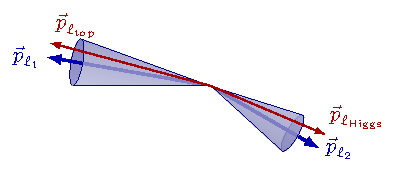
\includegraphics[width=\linewidth]{Chapter5_tHq/LeptAssociation/LepAssignement_2Matches_Type1}
	  \caption{Esdeveniment amb un etiquetatge vàlid del Tipus$\,$1 amb les dues correspondències.}
	  \label{fig:resum:tH:LepAssign:Match:Type1}
	\end{subfigure} 
	\begin{subfigure}{.49\textwidth}
	  \centering
	  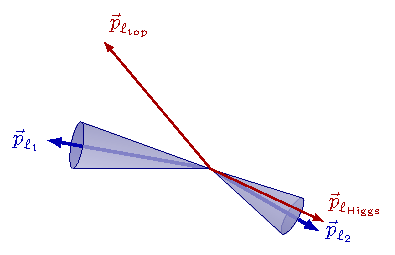
\includegraphics[width=\linewidth]{Chapter5_tHq/LeptAssociation/LepAssignement_1Match_Higgs_subleading}
	  \caption{Esdeveniment amb una sola correspondència. Ací no hi ha un etiquetatge vàlid.}
	  \label{fig:resum:tH:LepAssign:Match:Type2}
	\end{subfigure}
	\caption{Diferents escenaris per a l'associació de  leptons lleugers a nivell de reconstrucció (fletxa blava) i 
	a nivell de partons (fletxa roja). Cal notar que les etiquetes $\Pl_{\text{top}}$ i $\Pl_{\text{Higgs}}$ només 
	estan disponibles per a les partícules a nivell de partons.}
	\label{fig:resum:tH:LepAssign:Match}
	\end{figure}
	
	
	\item \textbf{Determinación de variables per la BDT}: La selecció de característiques d'entrada a nivell de reconstrucció 
	amb capacitat discriminatòria entre els Tipus$\,$1 i Tipus$\,$2. Aquestes variables no poden ser utilitzades després com 
	a entrades en els BDTs per a la definició de regions. Les variables utilitzades a la $\text{BDT}^{\text{OrigenLep}}$ són les 
	presentades a la Taula~\ref{tab:chap:tH:LepAssign:Vars}. Les distribucions d'aquestes variables poden observar-se a
	l'Apendix~\ref{chap:Appendix:BDT_Variables:LepAssignment}.
	
\begin{table}[htbp!]
\centering
\begin{adjustbox}{max width=0.95\textwidth}
\begin{tabular}{l|l|c}
\toprule
Variable & Significat & $<S^{2}>$ ($\times 0.1$) \\
\midrule
$m^{\text{opt1}}_{\text{vis}}(H)$ & Massa combinada del \tauhad i el $\ell_{1}$. & $3.734$ \\
$\Delta \eta(\tauhad, \ell_{1})$ & $\Delta \eta$ entre el \tauhad i el $\ell_{1}$. & $2.457$ \\\
$m^{\text{opt2}}_{\text{vis}}(H)$ & Massa combinada del \tauhad i el $\ell_{1}$. & $2.025$ \\
$\Delta \eta(\tauhad, \ell_{2})$ & $\Delta \eta$ entre el \tauhad i el leptó lleuger secundari. & $1.864$ \\
$m^{\text{opt1}}_{\text{pred}}(t)$ & Massa del quark top reconstruida amb el jet etiquetat $b$, el $\ell_{1}$ i el $\nu_{\ell_{1}}$. & $1.596$\\
$\dR(b \text{-tagged jet}, \ell_{1})$ & $\dR$ entre el jet etiquetat $b$ i el $\ell_{1}$. & $1.142 $ \\
$m^{\text{opt2}}_{\text{pred}}(t)$ & Massa del quark top reconstruida amb el jet etiquetat $b$, el $\ell_{2}$  i el $\nu_{\ell_{2}}$. & $1.104$ \\
$\dR(b\text{-tagged jet}, \ell_{2})$ & $\dR$ entre el jet etiquetat $b$ i el leptó lleuger secundari. & $1.009$ \\
$\Delta \eta(\text{closest }b\text{-tagged jet}, \ell_{1})$ & $\Delta \eta$ entre el $\ell_{1}$l i el jet etiquetat $b$ més pròxim a aquest leptó. & $0.740$ \\
\bottomrule
\end{tabular}
\end{adjustbox}
\caption{Variables utilitzades a l'entrenament de la a $\text{BDT}^{\text{OrigenLep}}$. 
El poder de separació ($<S^{2}>$) es presenta a la tercera columna.}
\label{tab:chap:tH:LepAssign:Vars}
\end{table}
	
	
	
 	\item \textbf{Optimització d'hiperparàmetres del model}: L'optimització dels hiperparàmetres d'entrenament és 
	un element clau per a augmentar l'eficàcia del model. En el cas de la $\text{BDT}^{\text{OrigenLep}}$, els paràmetres 
	seleccionats es mostren a la Taula~\ref{tab:resum:tH:LepAssign:Hyperparams}. Aquests valors òptims s'han 
	determinat mitjançant una cerca en retícula. En referència a la decisió sobre com tractar els pesos negatius 
	(excloure'ls o incloure'ls en l'entrenament), els tests indiquen que un entrenar només pesos positius ofereix un millor 
	rendiment. Els histogrames a la Figura~\ref{fig:Resum:NegWeights:Distributions} mostren que les distribucions 
	són similars utilitzant tots els esdeveniments o només els esdeveniments amb pesos positius, la qual cosa indica que 
	excloure els pesos negatius de l'entrenament no introdueix cap biaix en el model final.	
	
	
	\begin{figure}
\centering
\begin{subfigure}{.44\textwidth}
  \centering
  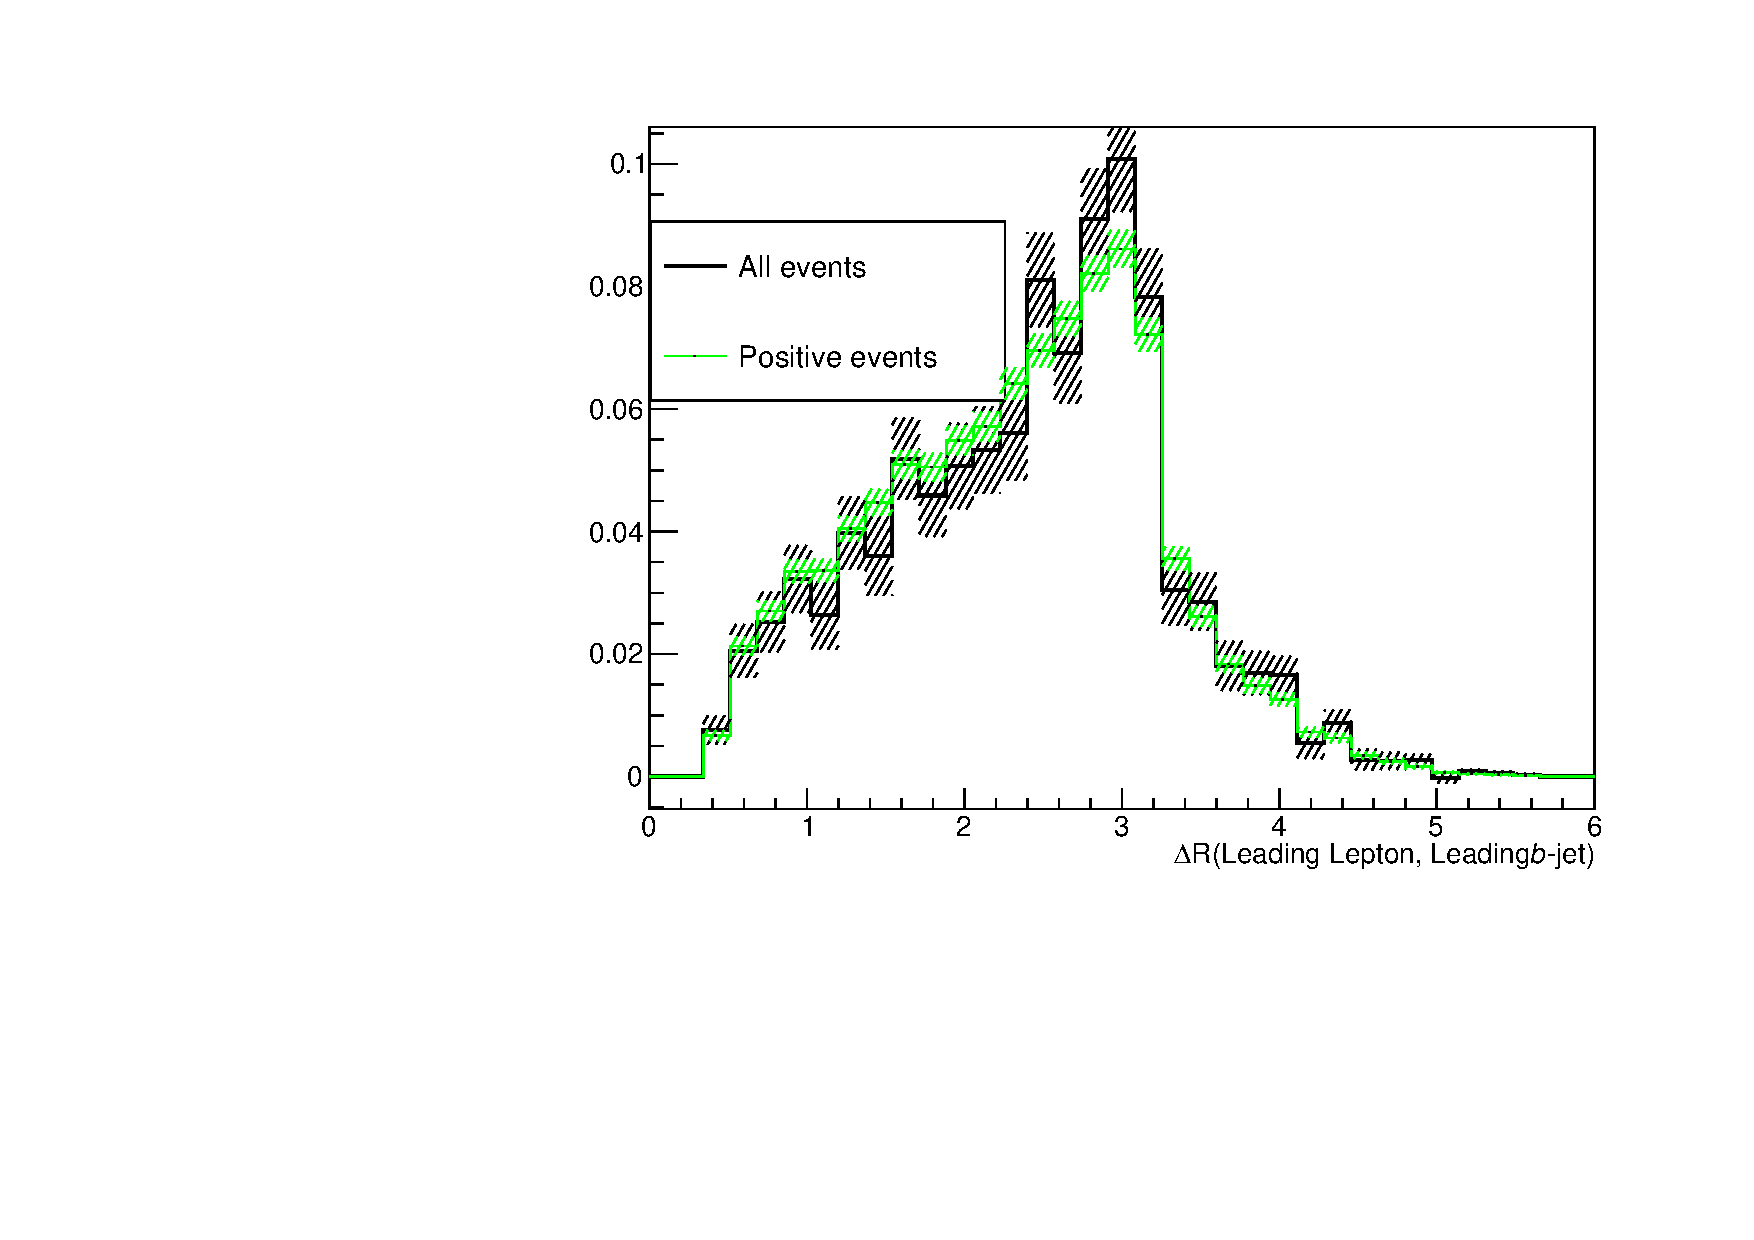
\includegraphics[width=.99\linewidth]{Appendices/Appendix_NegativeWeigts/PosVsAll_SS_err_deltaR_b_LightLep1}
  \caption{$\Delta R$ entre el jet etiquetat com a $b$ i el $\ell_{1}$.}
\end{subfigure}%
\begin{subfigure}{.44\textwidth}
  \centering
  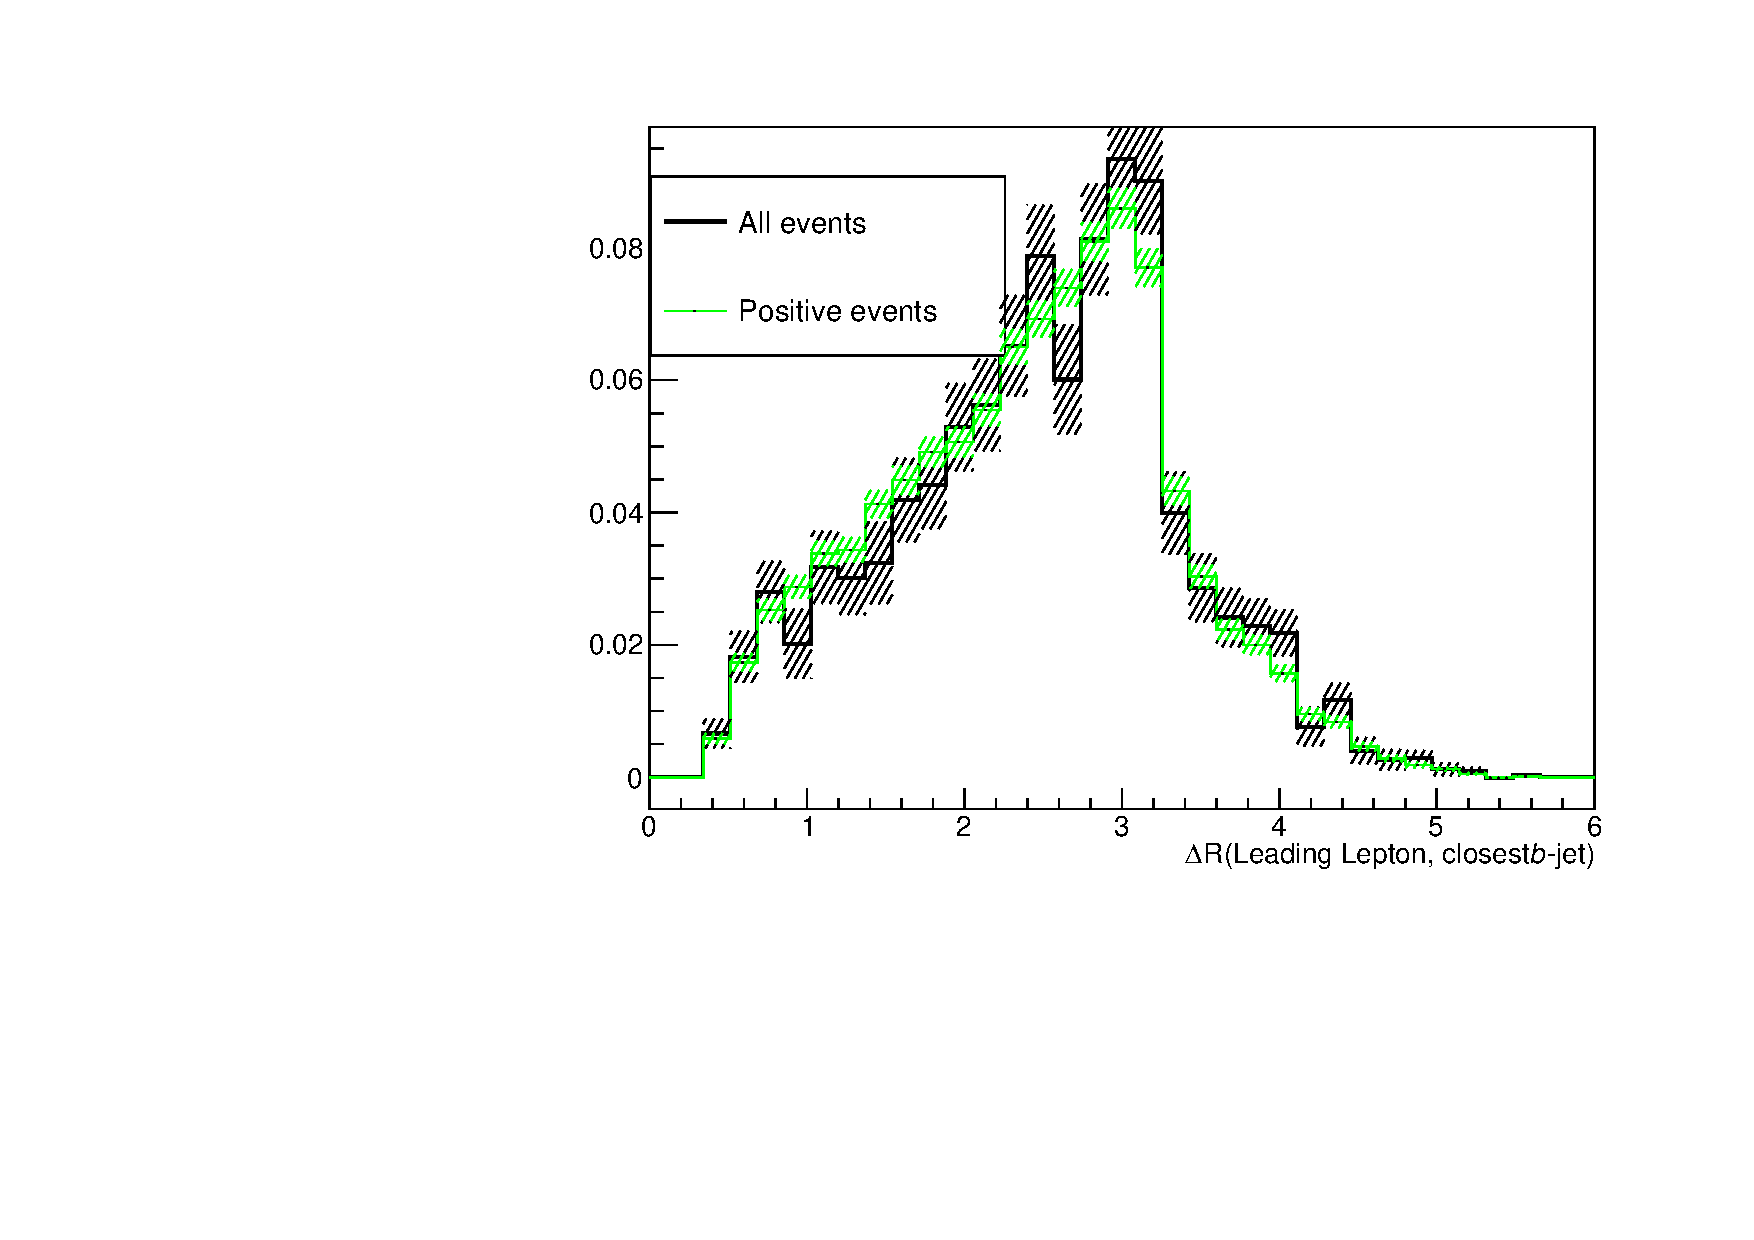
\includegraphics[width=.99\linewidth]{Appendices/Appendix_NegativeWeigts/PosVsAll_SS_err_DeltaRLeadingLeptonClosestBjet}
  \caption{$\Delta R$ entre el $\ell_{1}$ i el  jet etiquetat com a $b$ més pròxim a aquest leptó.}
\end{subfigure} \hfill%

\begin{subfigure}{.44\textwidth}
  \centering
  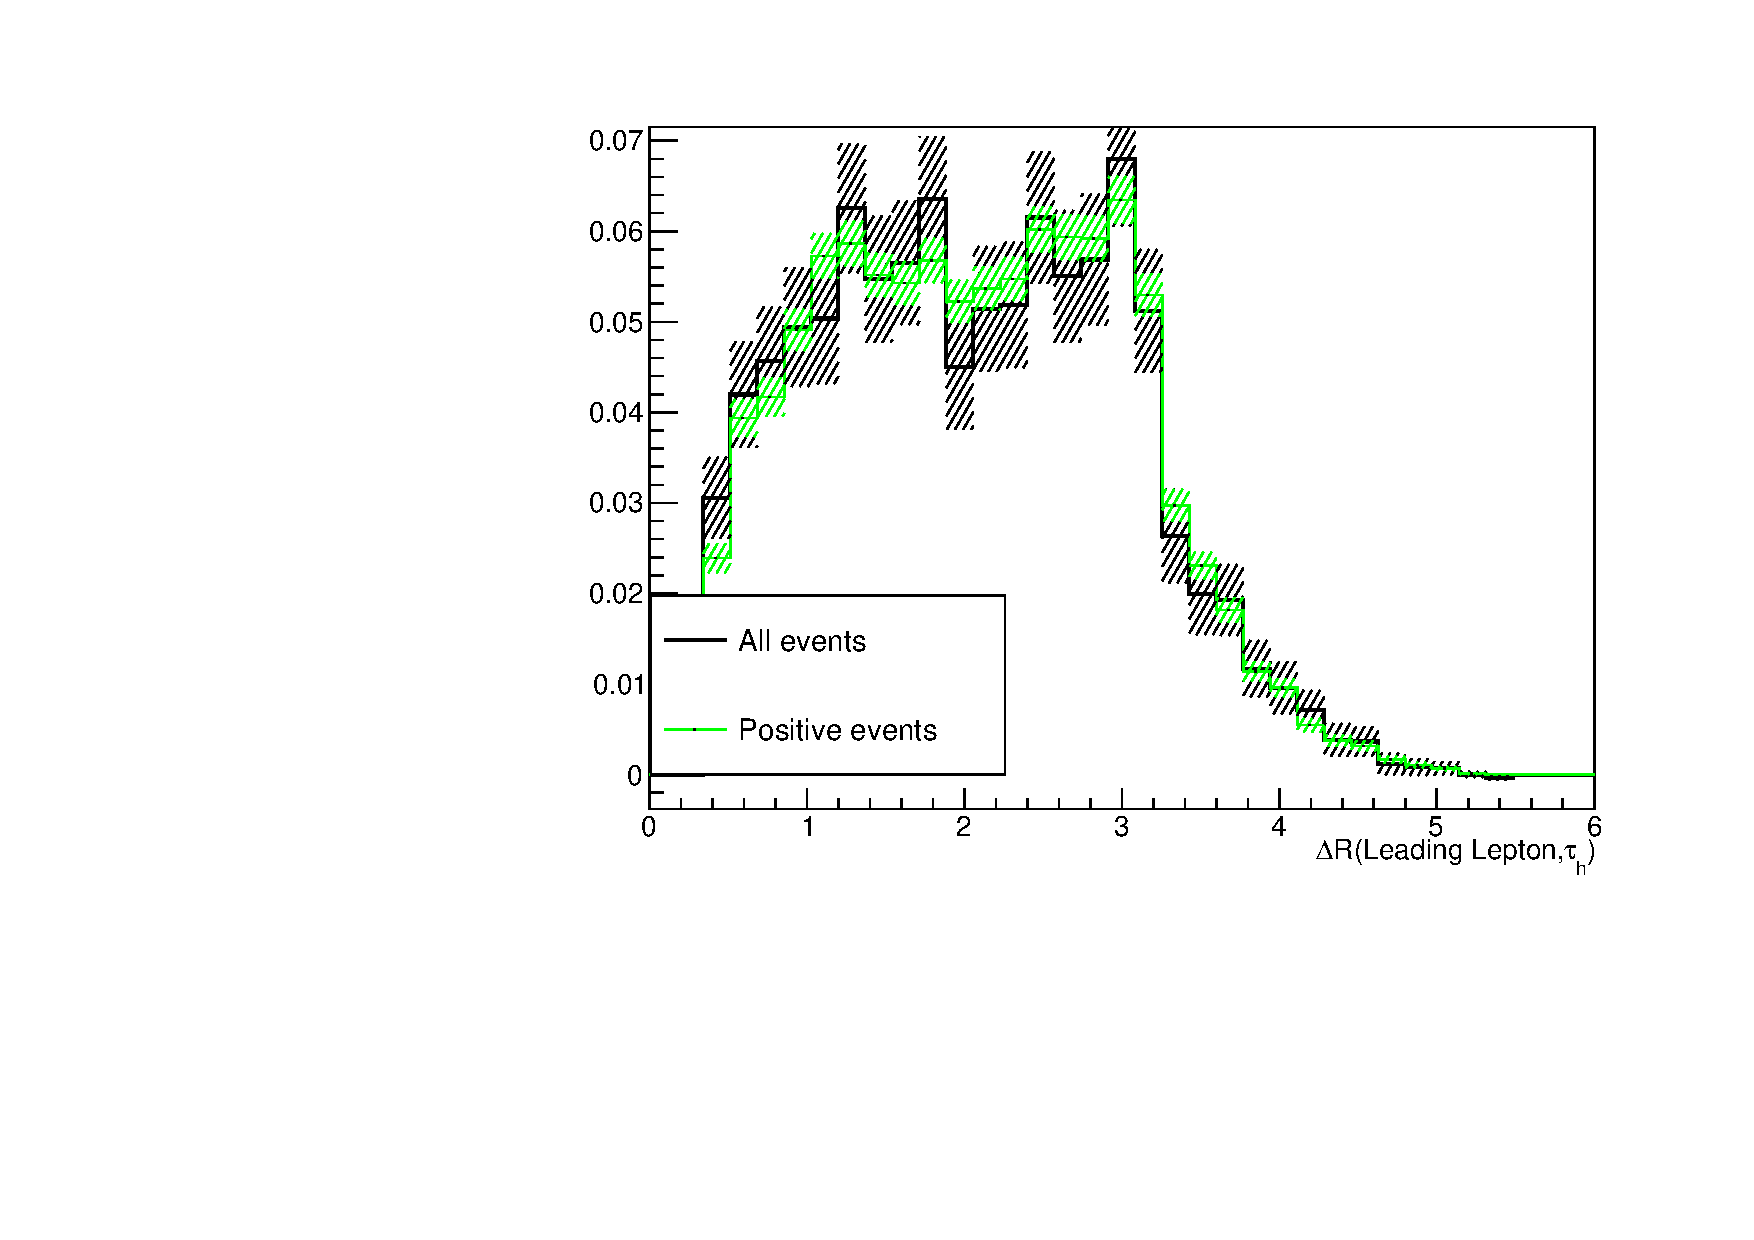
\includegraphics[width=.99\linewidth]{Appendices/Appendix_NegativeWeigts/PosVsAll_SS_err_deltaR_tau_LightLep1}
  \caption{$\Delta R$ entr el \tauhad i $\ell_{1}$}
\end{subfigure}%
\begin{subfigure}{.44\textwidth}
  \centering
  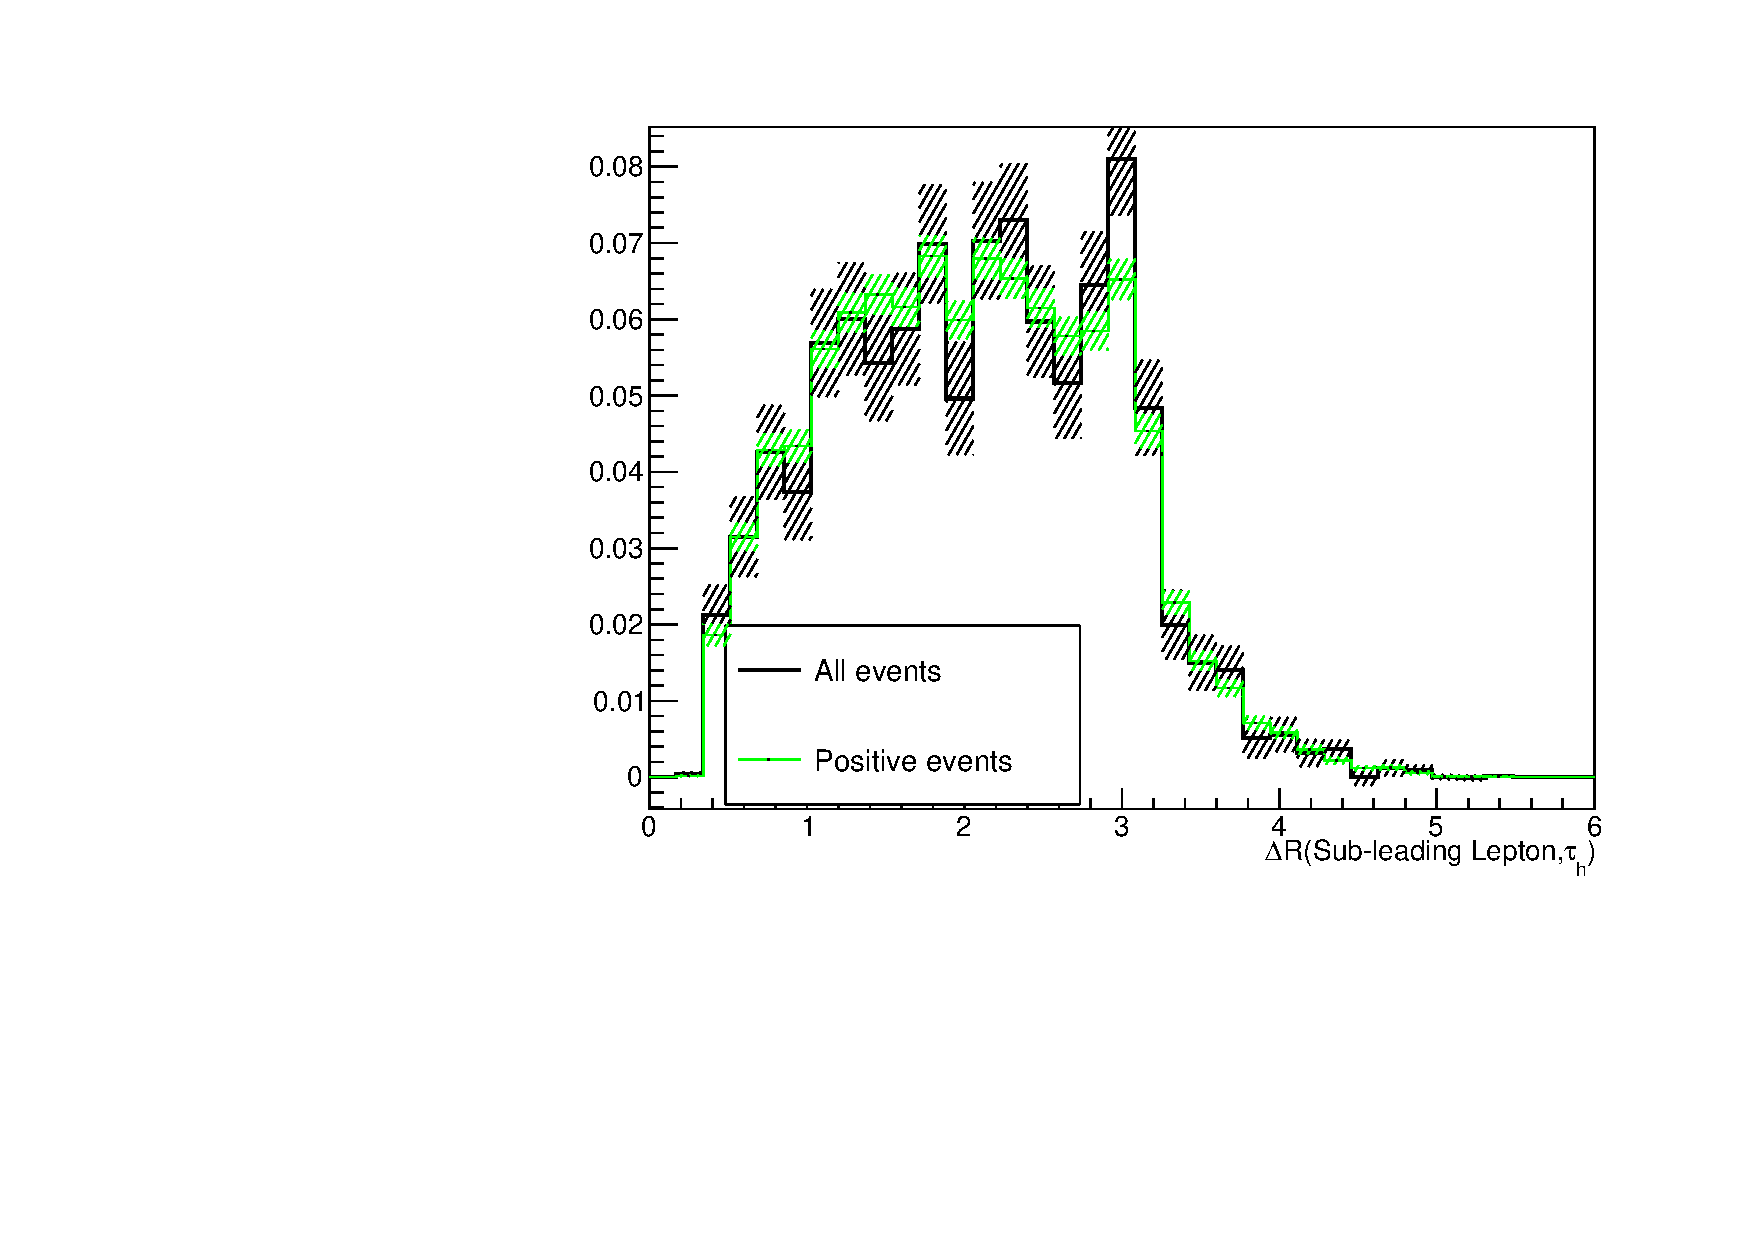
\includegraphics[width=.99\linewidth]{Appendices/Appendix_NegativeWeigts/PosVsAll_SS_err_deltaR_tau_LightLep2}
  \caption{$\Delta R$ entre el \tauhad i $\ell_{2}$}
\end{subfigure}%
\caption{Distribucions normalitzades de variables cinemàtiques utilitzades a la $\text{BDT}^{\text{OrigenLep}}$ a l'espai de fases
corresponent al canal \dilepSStau. En negre es mostren tots els esdeveniments i en verd només esdeveniments amb pesos positius.
Per a cada bin, la banda d'error es calcula com l'arrel quadrada de la suma quadràtica dels pesos.}
\label{fig:Resum:NegWeights:Distributions}
\end{figure}
	
\begin{table}[htbp!]
\centering
\begin{tabular}{l|l|l}
\toprule
Hiperparàmetre & Valor & Significat \\
\midrule
\texttt{Type} & Gradient & Algoritme per al \textit{boosting} per als arbres. \\
\texttt{MaxDepth} & 3 & Profunditat màxima de l'arbre. \\
\texttt{Shrinkage} & 0.2 & Taxa d'aprenentatge per l'algoritme. \\
\texttt{NTrees} & $10^3$ & Nombre d'arbres en el mètode. \\
\multirow{2}{*} {\texttt{nCuts}} & \multirow{2}{*}{40} & Nombre de punts a testejar per trobar \\
& &										  el tall òptim en la divisió del node. \\
\texttt{NegWeights} & Ignore neg & Ús dels pesos negatius a l'entrenament.\\
\bottomrule
\end{tabular}
\caption{Valors dels hiperparàmetres utilitzats per gestionar l'entrenament de la $\text{BDT}^{\text{OrigenLep}}$.
La resta d'hiperparàmetres utilitzen el seu valors per defecte.}
\label{tab:resum:tH:LepAssign:Hyperparams}
\end{table}
	
	%\item \textbf{Ús de pesos negatius}: L'elecció de l'estratègia de tractament de pesos negatius
	%\pablo{posar un plot dels pesos negatius}
	
	\item \textbf{Entrenament del model}: L'entrenament supervisat del model per classificar esdeveniments segons
	l'origen del leptó lleuger crea un discriminant que es presenta a la Figura~\ref{fig:resum:Assignment:ElModel}.
	Per tal de evaluar la capacitat predictiva d'un model estadístic, la validació creuada $K$-fold és utilitzada amb cinc \textit{folds}.

	\begin{figure}[h]
 	 \begin{subfigure}[h]{0.45\linewidth}
  	\includegraphics[width=\linewidth]{Chapter5_tHq/LeptAssociation/dileptau_LepAssignment_BDT_Score_ALL_test_GoodLegend.pdf}
	\caption{}
	\label{fig:resum:Assignment:ROC_and_Score:kfoldeo}
 	 \end{subfigure}
	 \begin{subfigure}[h]{0.55\linewidth}
	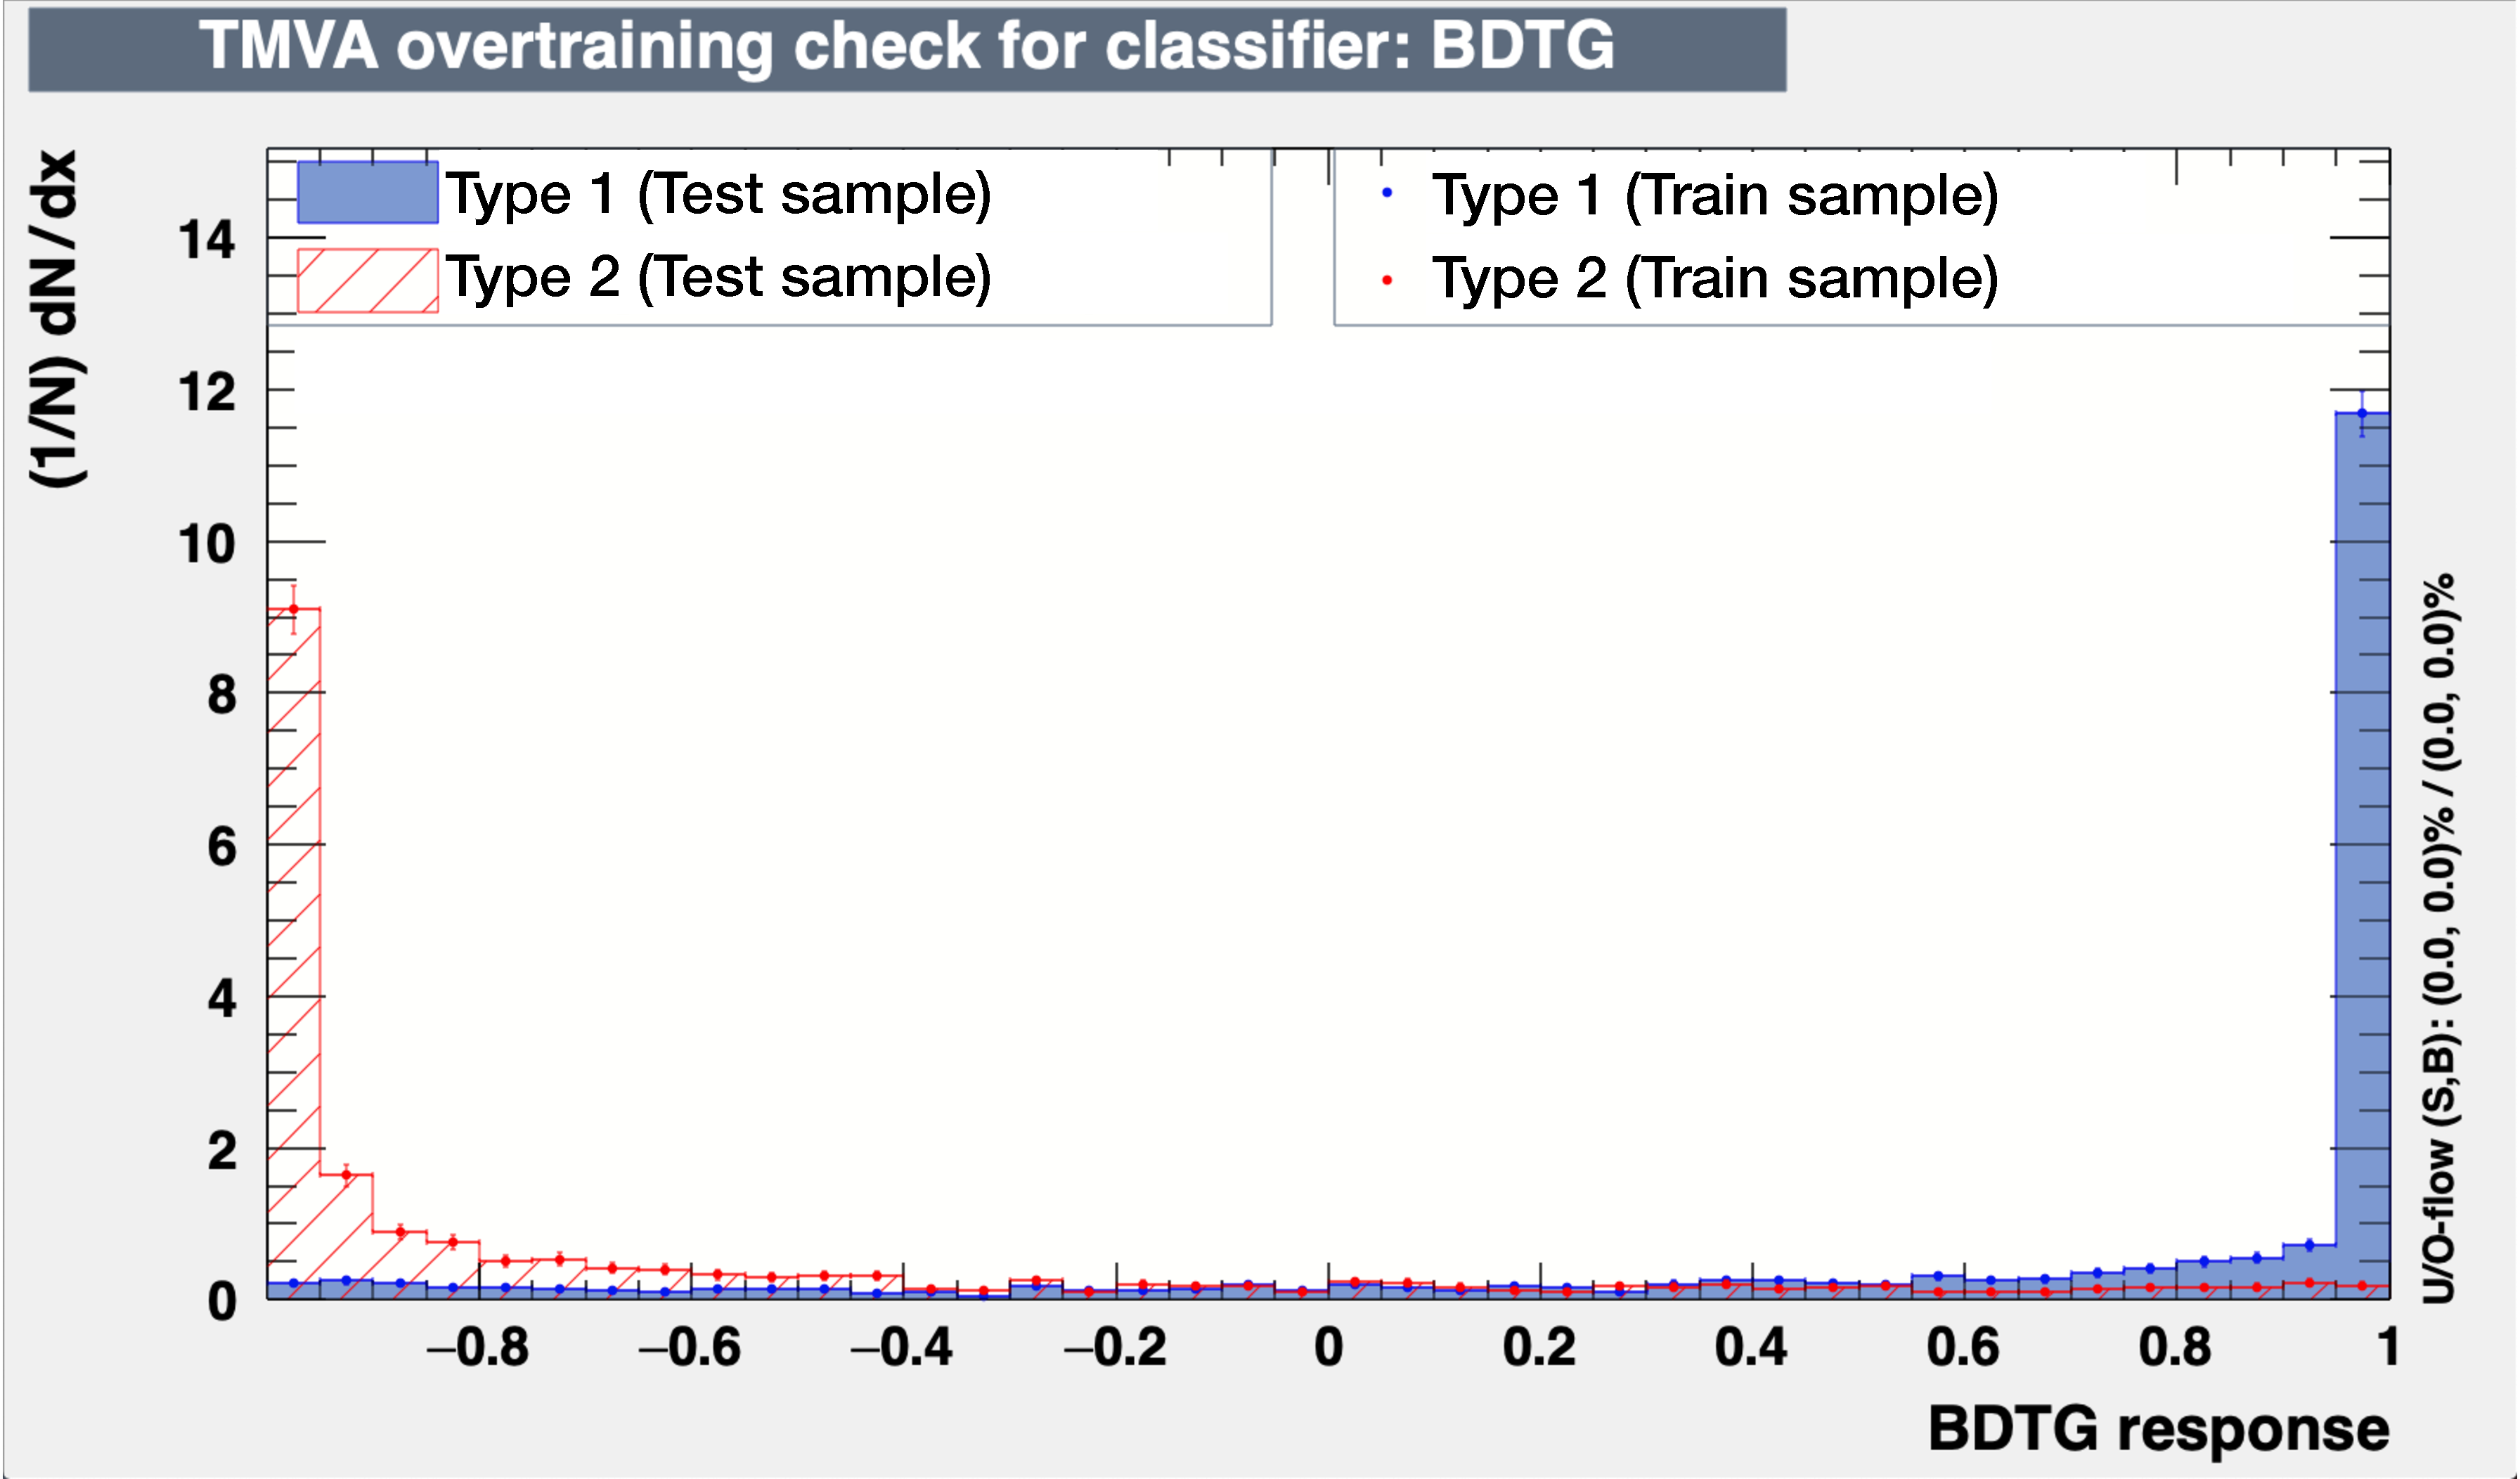
\includegraphics[width=\linewidth]{Chapter5_tHq/LeptAssociation/Dileptau_BDT_Based_Assignment_Score_General}
	\caption{} 
	\label{fig:resum:Assignment:ROC_and_Score:Score}
 	 \end{subfigure}%
	\caption{Distribució de  la $\text{BDT}^{\text{OrigenLep}}$. En la figura (a) els cinc models del $K$-folding són comparats 
	a les mostres de test. En (b) el model final és presentat comparant la distribució d'esdeviments de Tipus$\,$1 (blau) i de 
	Tipus$\,$2 (roig).} 
	\label{fig:resum:Assignment:ElModel}
	\end{figure}
	
	
	\item \textbf{Injecció del model}: L'últim pas consisteix en l'aplicació del model sobre les dades i en 
	la determinació del llindar de classificació òptim. Una cerca lineal troba que 
	$\text{BDT}^{\text{OrigenLep }}=-0.315$ és el punt òptim per discriminar esdeveniments de 
	Tipus$\,$1 i Tipus$\,$2. 

\end{enumerate}

Una vegada establit l'origen del leptó, en comptes de fer servir $\Pl_{1}$ i $\Pl_{2}$, les variables 
per a la discriminació entre senyal i fons fan servir $\Pl_{\text{top}}$ i $\Pl_{\text{Higgs}}$. Definir 
els leptons segons el seu origen, en lloc de la seua $p_T$, permet crear variables més eficaces 
per a la discriminació. A la Taula~\ref{tab:resum:Assignment:MethodsSummary}, la tècnica basada 
en la $\text{BDT}^{\text{OrigenLep}}$ es compara amb un mètode alternatiu que consisteix a aplicar 
dos requisits cinemàtics. Com es pot apreciar, l'eficàcia de classificació del mètode descrit ací és superior.


\begin{table}[h]
\centering
\resizebox{\textwidth}{!}{
\begin{tabular}{l|llc|}
\cline{2-4}
& \multicolumn{3}{c|}{Precisió de l'assignació de l'origen del lepton lleuger} \\ \cline{2-4}
& \multicolumn{1}{l|}{Total (100\%)} & \multicolumn{1}{l|}{$H\rightarrow \tau \tau$ (83.08\%)} & $H\rightarrow WW$ (16.92\%) \\ \midrule
\multicolumn{1}{|l|}{$\text{BDT}^{\text{OrigenLep}}$} & \multicolumn{1}{c|}{88.39} & \multicolumn{1}{c|}{88.44} & 88.18 \\ \midrule
\multicolumn{1}{|l|}{Mètode basat en talls} & \multicolumn{1}{c|}{83.86} & \multicolumn{1}{c|}{84.24} & 81.80 \\ \bottomrule
\end{tabular}}
\caption{Precisió calculada comparant la predicció del mètode amb el valor real.
El valor real s'ha obtingut utilitzant l'etiquetatge amb l'informació a nivell de partons.
Aquest etiquetatge està disponible per a \Htautau i \HWW però no per \HZZ. 
Només s'han utilitzat esdeveniments on hi havia una correspondència entre els 
leptons a nivell de reconstrucció i a nivell de partons.}
\label{tab:resum:Assignment:MethodsSummary}
\end{table}



\subsubsection{Reconstrucció del sistema}
\label{chap:resumen_val:tHq:Senyal:reco}
La reconstrucció precisa del moment i la massa del quark top i del bosó de Higgs és una tasca complicada
a causa de la presència de, almenys, quatre neutrins en l'estat final.
En aquest treball, l'estratègia utilitzada per a reconstruir completament el top i el bosó de Higgs consisteix primer
a reconstruir el sistema del quark top i després la cadena del bosó de Higgs. Com que coneixem
el \MET total, si l'energia mancant és reconstruïda per al quark top, es pot fer servir:
\begin{equation*}
\overrightarrow{E}_{\text{T}}^{\text{miss}} (\text{total}) = \overrightarrow{E}_{\text{T}}^{\text{miss}} (\text{Higgs}) + \overrightarrow{E}_{\text{T}}^{\text{miss}} (\text{top})
\end{equation*}
per a obtindre $\overrightarrow{E}_{\text{T}}^{\text{miss}}$ del sistema del Higgs.

Llavors, el primer pas és reconstruït el quark top.
Com que al seu sistema de desintegració hi ha un neutrí ($\nu_{\text{top}}$) com a mínim, cal estudiar la hipòtesi
per a aconseguir $\overrightarrow{p}(\nu_{\text{top}})$. Les relacions aconseguides a través d'un ajust per a conéixer
$\overrightarrow{E}_{\text{T}}^{\text{miss}}$(top) són:
\begin{align*}
\begin{split}
p^{\text{miss}}_{\text{T}, \nu_{\text{top}}} &= \frac{1615.18 \text{GeV}^{2}}{p_{\text{T}, \ell_{\text{top}}}}\, , \\
\phi^{\text{miss}}_{\nu_{\text{top}}} &= \phi_{\ell_{\text{top}}} \pm \frac{\pi}{2} \, ,
\end{split}
\end{align*}
sent $p_{\text{T}, \ell_{\text{top}}}$ i $\phi_{\ell_{\text{top}}}$ el moment transvers i l'angle azimutal del $\ell_{top}$.

Una vegada obtingut l'energia transversa mancant del sistema del quark top s'utilitza el mètode de la Calculadora de Massa Perduda (MMC),
originalment desenvolupat per reconstruir la massa i moment del bosó de Higgs a l'anàlisi \Htautau~\cite{ELAGIN2011481}.


%%%%%%%%%%%%%%%%%
%   Estimació del fons   %
%%%%%%%%%%%%%%%%%
\subsection{Estimació del fons}
\label{chap:resumen_val:tHq:Fons}
En la nostra anàlisi, diferenciem els esdeveniments de fons en dos tipus: ``reductible'' i ``irreductible''.
\begin{itemize}
	\item \textbf{Fons irreductibles}: Es refereixen a processos amb estats finals idèntics al senyal,
	Aquesta mena de fons no es poden distingir dels processos \tHq a través de la multiplicitat d'objectes físics reconstruïts.
	En la nostra anàlisi són Diboson ($VV$), \tW, \ttZ, \ttH, \ttW i \tZq.
	\item \textbf{Fons reductibles}: Originats per errors de reconstrucció, on objectes són incorrectament identificats
	com a part del senyal. Al canal \dileptau, predominen els esdeveniments identificats consistents en
	jets erròniament identificats com \tauhad. Açó genera els fons de \ttbar i \Zjets. També inclouen processos amb $VV$ i certes produccions de \ttX.
\end{itemize}

 \pablo{Explicar breument el mètode de l'ajust de plantilla i el mètode de recompte.}


\FloatBarrier
%%%%%%%%%%%%%%%%%
%   Selecció d'esdeveniments   %
%%%%%%%%%%%%%%%%%
\subsection{Selecció d’esdeveniments}
\label{chap:resumen_val:tHq:Seleccio}
La selecció d'esdeveniments consisteix en l'aplicació d'un conjunt de condicions que ens 
permeten separar el senyal del fons. D'aquesta manera, definim una regió de l'espai de 
fases enriquida amb esdeveniments de senyal. Aquesta regió es denomina regió de senyal (SR).

El punt de partida és la regió de preselecció (PR), on els objectes físics són seleccionats 
segons l'acceptació del detector. Els requisits de PR estan resumits a la Taula~\ref{tab:resum:EventSelection:Preselection} 
i el nombre d'esdeveniments a la regió de PR es presenta a la Taula~\ref{tab:resum:EventSelection:Preselection}
tant per a tot \dileptau com per als dos canals que el componen.

A continuació, es defineixen variables discriminants i s'utilitzen
com a característiques d'entrada per a un BDT que distingís entre esdeveniments de senyal i 
fons, creant un discriminant.

\begin{table}[h]
\begin{adjustbox}{max width=0.99\textwidth}
\begin{tabular}{llll}
\toprule
Objecte & Multiplicitat & Moment lineal & Pseudorapidesa                                                    \\  \midrule
\multirow{2}{*}{Leptons lleugers} & \multirow{2}{*}{$n(\Pe / \Pmu)=2$} & $\pT(\Pe)>14\,$GeV            & $|\eta(\Pe)|<2.47$,\, $|\eta(\Pe)| \notin [1.37,\, 1.52]$         \\
                               &                                    & $\pT(\Pmu)>14\,$GeV           & $|\eta(\Pmu)|<2.50$                                              \\
au hadrònic             & $n(\tauhad)=1$        & $\pT(\tauhad)>20\,$GeV        & $|\eta(\tauhad)|<2.50$,\, $|\eta(\tauhad)| \notin [1.37, 1.52]$ \\
Jets                           & $n(\text{jet})=[2,\,6]$    & $\pT(\text{jet})>20\,$GeV      & $|\eta(\text{jet})|<4.5$                                               \\
Jets etiquetats $b$              & $n(\bjet)=[1,\,2]$          & $\pT(\bjet)>20\,$GeV             & $|\eta(\bjet)|<2.5$                                              \\
\MET                         &                                 & $\pT(\MET)\in[5,\,800]\,$GeV &                                        \\ 
\bottomrule                         
\end{tabular}
\end{adjustbox}
\caption{Requeriments de preselecció. Per als leptons principal i secundari s'aplica 
un tall addicional en $\pT$: $\pT(\Plepton_{1})>27,$GeV i $\pT(\Plepton_{2})>20,$GeV.
El signe relatiu de la càrrega elèctrica dels leptons lleugers també s'utilitza en la preselecció 
per separar els canals \dilepSStau i \dilepOStau.}
\label{tab:resum:Preselection}
\end{table}

\begin{table}[h]
\centering
\begin{tabular}{l| c| c| c}
\toprule
Procés			& \dileptau     			& \dilepOStau     	& \dilepSStau \\ \midrule
\tHq         			&  $3.2 \pm 0.8$    		&  $1.9 \pm 0.5$    	&  $1.22 \pm 0.34$ 	\\
\tWH         		&  $3.4 \pm 2.5$    		&  $2.4 \pm 1.8$    	&  $1.0 \pm 0.7$   	\\
\ttbar         		&  $5710 \pm 350$   		&  $5690 \pm 350$   	&  $25 \pm 10$     	\\
\Zjets         		&  $3800 \pm 1400$  	&  $3800 \pm 1400$ &  $0.7 \pm 0.4$   	\\
\ttW   			&  $130 \pm 330$    		&  $90 \pm 230$     	&  $40 \pm 100$   	\\
\ttH   			&  $86 \pm 29$      		&  $61 \pm 20$      	&  $25 \pm 9$      	\\
\ttZ        			&  $160 \pm 29$     		&  $139 \pm 26$     	&  $21 \pm 4$      	\\
\tWZ              		&  $22 \pm 16$      		&  $19 \pm 14$      	&  $2.6 \pm 2.1$   	\\
\tZq         			&  $45 \pm 7$       		&  $40 \pm 6$       	&  $5.4 \pm 0.9$   	\\
\tW              		&  $260 \pm 40$     		&  $260 \pm 40$     	&  $1.2 \pm 1.0$   	\\
Diboson          		&  $190 \pm 130$    		&  $180 \pm 130$    	&  $10 \pm 6$      	\\
Fons menors      	&  $16 \pm 9$       		&  $14 \pm 8$      	&  $1.8 \pm 1.1$   	\\ \midrule
Fons total 			&  $10400 \pm 1500$ 	&  $10300 \pm 1500$&  $140 \pm 110$  	\\ \midrule
\StoB (\%)     		& 0.031				&    	0.018		&   0.89  			\\ \midrule
Significància 		& 0.031				&	0.019		&   0.104	   		\\ \bottomrule
\end{tabular}
\caption{Nombre d'esdeveniments al nivell de PR per al canal \dileptau i els seus dos subcanals.
Les incerteses corresponen tant a l'error  estadístic com a les incerteses sistemàtiques (descrites a la Secció~\ref{sec:resum:Incerteses}).}
\label{tab:resum:EventSelection:Preselection}
\end{table}

Finalment, aplicant requisits sobre les sortides del BDT, es defineix la SR. També es poden 
definir regions de l'espai de fases enriquides amb processos d'un fons específic. Aquestes 
es coneixen com a regions de control (CR) o de validació (VR). La diferència entre CR i VR 
és que, mentre les primeres són considerades en els càlculs de l'ajust, les segones no ho són. 
Les SR, CRs i VRs són totes ortogonals entre si i són subespais de la PR

Per a distingir el procés de senyal \tHq dels fons i crear regions dedicades als fons,
es construeixen diversos BDTs de gradient per a la classificació binària:
\begin{itemize}
	\item BDT$(\tHq|{\text{OS}})$: Entrenat per a discriminar el procés \tHq de tots els fons simultàniament
		en el canal \dilepOStau. Aquest BDT es fa servir després per a definir la SR per a tHq en aquest canal.
	\item BDT$(\ttbar|{\text{OS}})$ Entrenat amb l'objectiu de separar \ttbar i \Zjets en el canal \dilepOStau. 
		S'utilitza per a definir les VRs per a aquests dos processos.
	\item BDT$(\tHq|_{\text{SS}})$: Entrenat per al canal \dilepSStau per a discriminar el procés \tHq de la resta 
		de processos.
\end{itemize}

Igual que per a l'assignació de l'origen del leptons lleugers, els passos per a entrenar 
aquests models són: l'elecció de variables, l'optimització d'hiperparàmetres, l'entrenament 
del propi model i la injecció de la puntuació del model. Ací també es fa servir $k$-folding amb
$k=5$ per a la validació creuada.

Els esdeveniments simulats amb pesos negatius representen aproximadament un 30\% del total.
Per al BDT$(\tHq|{\text{OS}})$ i BDT$(\ttbar|{\text{OS}})$, només s'usen els pesos positius.
Per al BDT$(\tHq|{\text{SS}})$, s'usa el valor absolut del pes a l'entrenament.
Aquesta elecció és preferida per l'escassetat d'esdeveniments en el canal \dilepSStau.

Pel que fa a la selecció de variables, aquestes són escollides per maximitzar el poder
de separació de la BDT. Un algoritme iteratiu construeix la llista de variables utilitzades
en cada BDT tenint en compte el valor que aporta cada variable al rendiment del model
i les seues correlacions amb les altres variables. El resultat d'aquest mètode dona lloc
a les tres llistes de variables presentades a la Figura~\ref{fig:resum:EventSelection:BDT:Rankings}.
La distribució de la variable més important de cada llista es mostra a la Figura~\ref{fig:resum:EventSelection:BDT:VariablesRelevants}.

\begin{figure}[h]
  \centering  
  \begin{subfigure}[b]{0.49\textwidth}
    \centering
    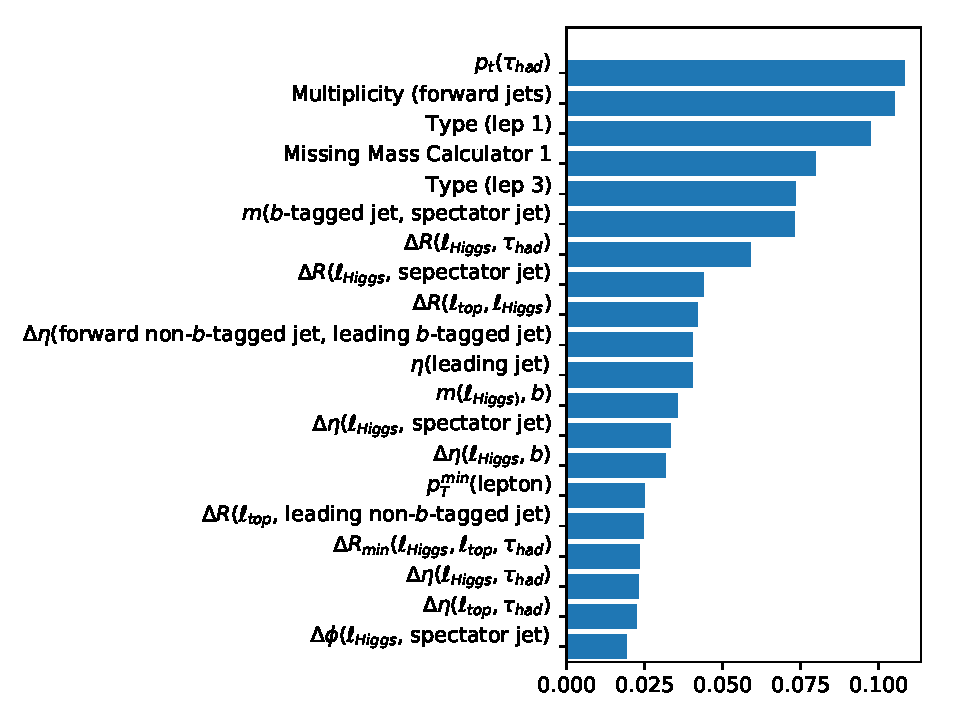
\includegraphics[width=\textwidth]{Chapter5_tHq/BDT_Results/Feature_importance_tHq_OS}
    \caption{BDT$(\tHq|_{\text{OS}})$.}
     \label{fig:Summary:EventSelection:BDT:Rankings:tHqOS}
  \end{subfigure}
  \hfill
  \begin{subfigure}[b]{0.49\textwidth}
    \centering
    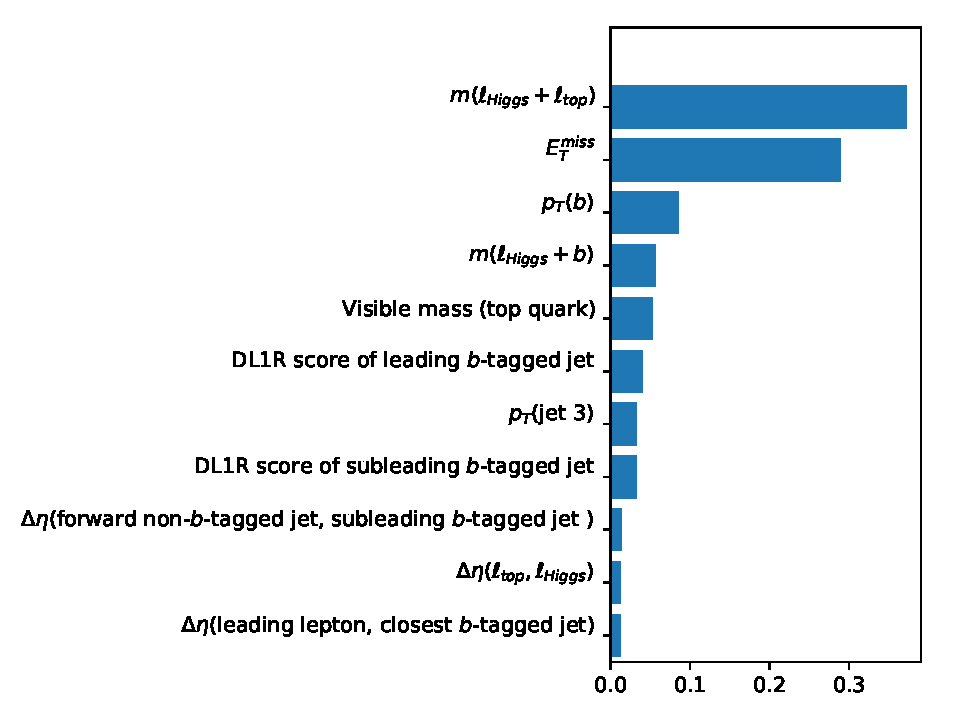
\includegraphics[width=\textwidth]{Chapter5_tHq/BDT_Results/Feature_importance_ttbar_OS}
    \caption{BDT$(\ttbar|_{\text{OS}})$}
     \label{fig:Summary:EventSelection:BDT:Rankings:ttbarOS}
  \end{subfigure}
    \hfill
  \begin{subfigure}[b]{0.49\textwidth}
    \centering
    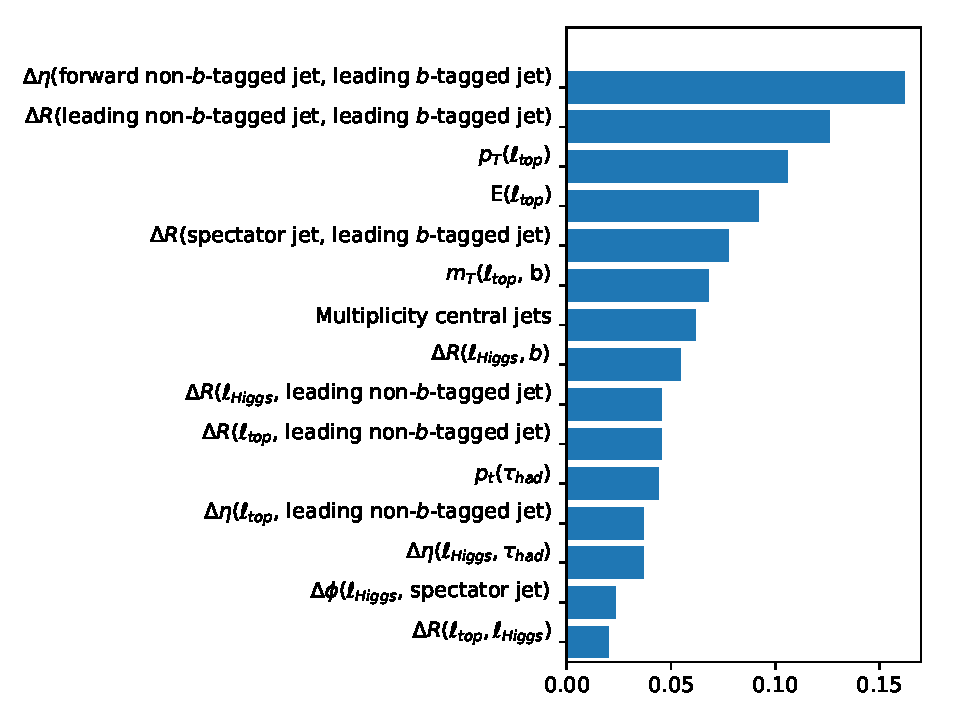
\includegraphics[width=\textwidth]{Chapter5_tHq/BDT_Results/Feature_importance_tHq_SS}
    \caption{BDT$(\tHq|_{\text{SS}})$}
     \label{fig:Summary:EventSelection:BDT:Rankings:tHqSS}
  \end{subfigure}
  \caption{Rànquing de variables per a cada BDT: a) BDT$(\tHq|_{\text{OS}})$, (b) BDT$(\ttbar|_{\text{OS}})$ 
  	      i (c) BDT$(\tHq|_{\text{SS}})$ Els rànquings s'han obtingut amb l'eina d'importància de característiques 
	      d'XGBoost. L'eix x correspon al valor que XGBoost dóna per a avaluar la precisió aportada per la 
	      variable al BDT.} 
  \label{fig:resum:EventSelection:BDT:Rankings}
\end{figure}


\begin{figure}[h]
  \centering  
  \begin{subfigure}[b]{0.49\textwidth}
    \centering
    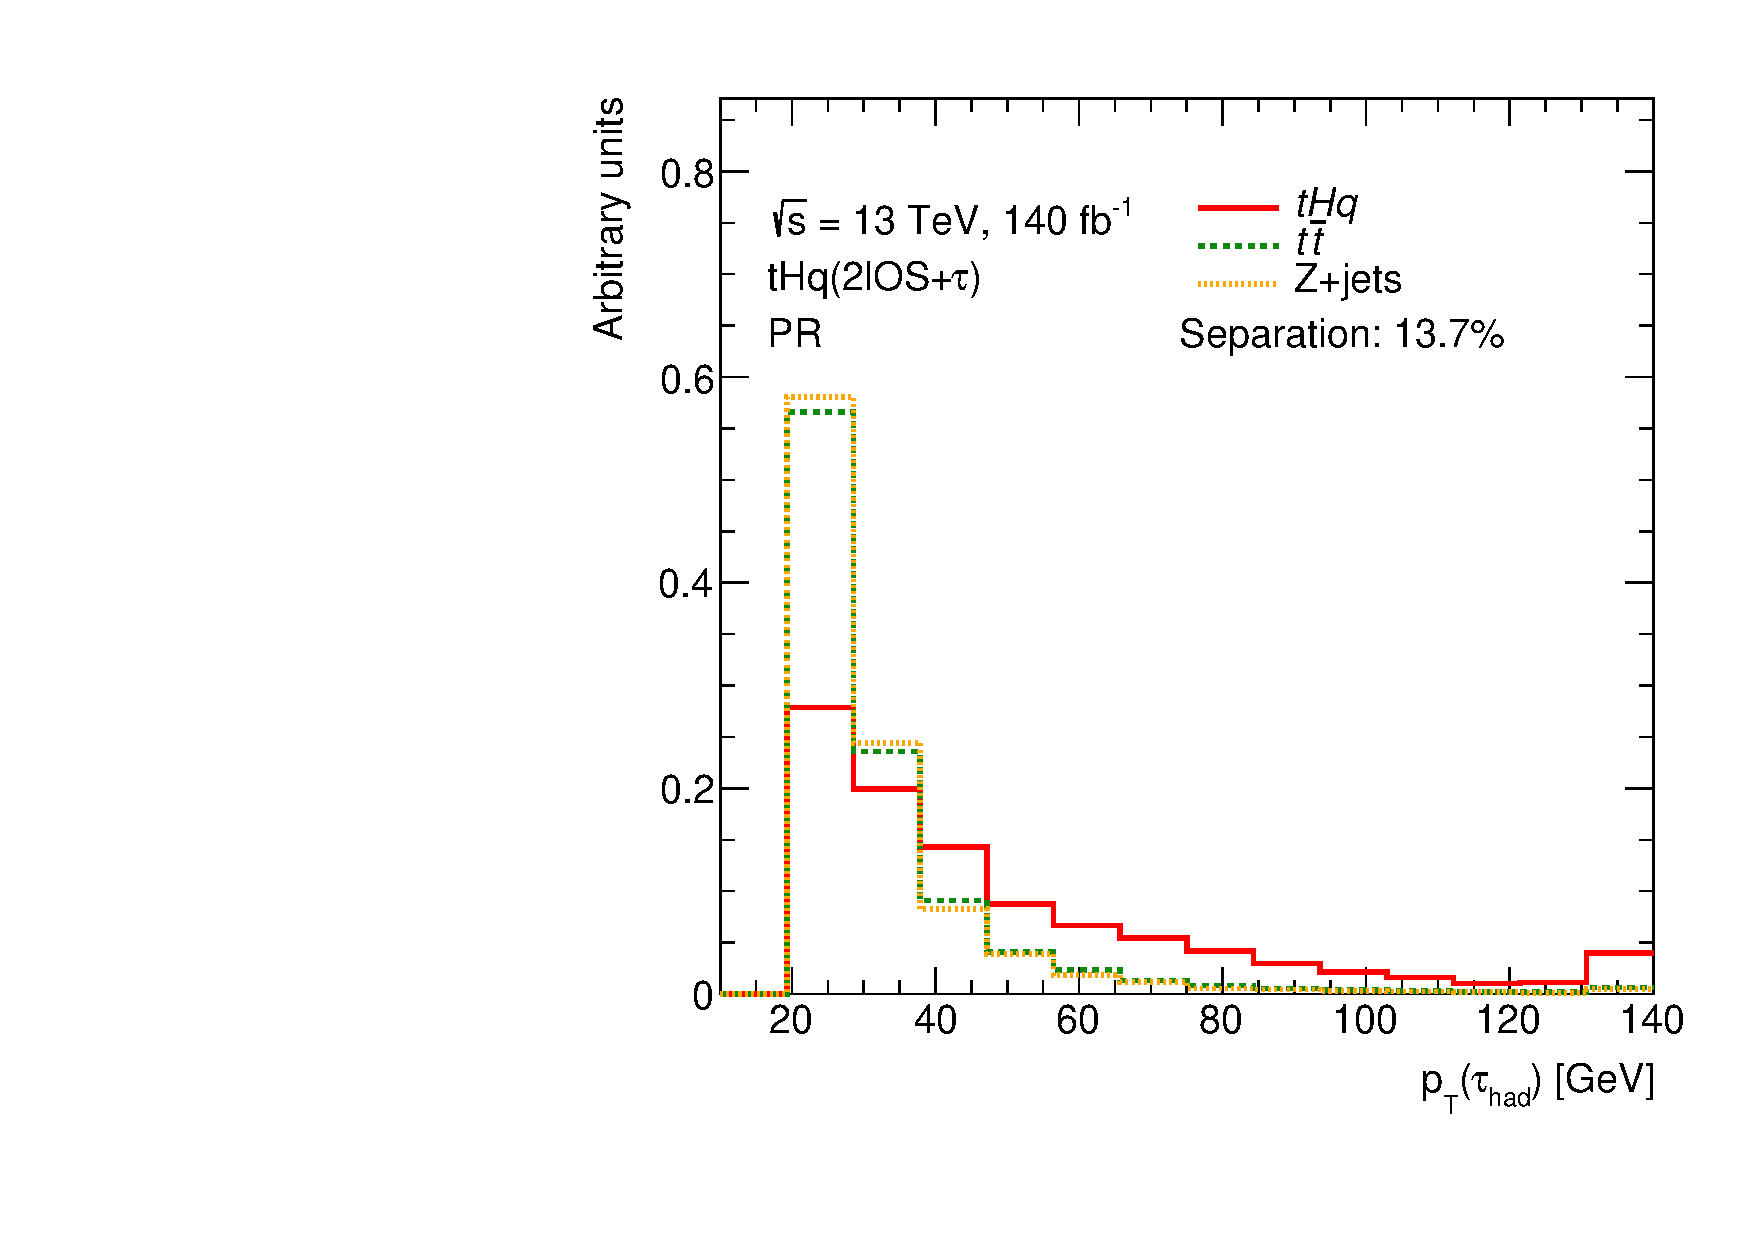
\includegraphics[width=\textwidth]{Chapter5_tHq/BDT_Results/BDT_Variables_tHq_OS/a01_PR_had_tau_pt_2L1TAU_OS}
    \caption{La variable més rellevant de la BDT$(\tHq|_{\text{OS}})$, el \pT del \tauhad.}
     \label{fig:resum:EventSelection:BDT:VariablesRelevants:tHqOS}
  \end{subfigure}
  \hfill
  \begin{subfigure}[b]{0.49\textwidth}
    \centering
    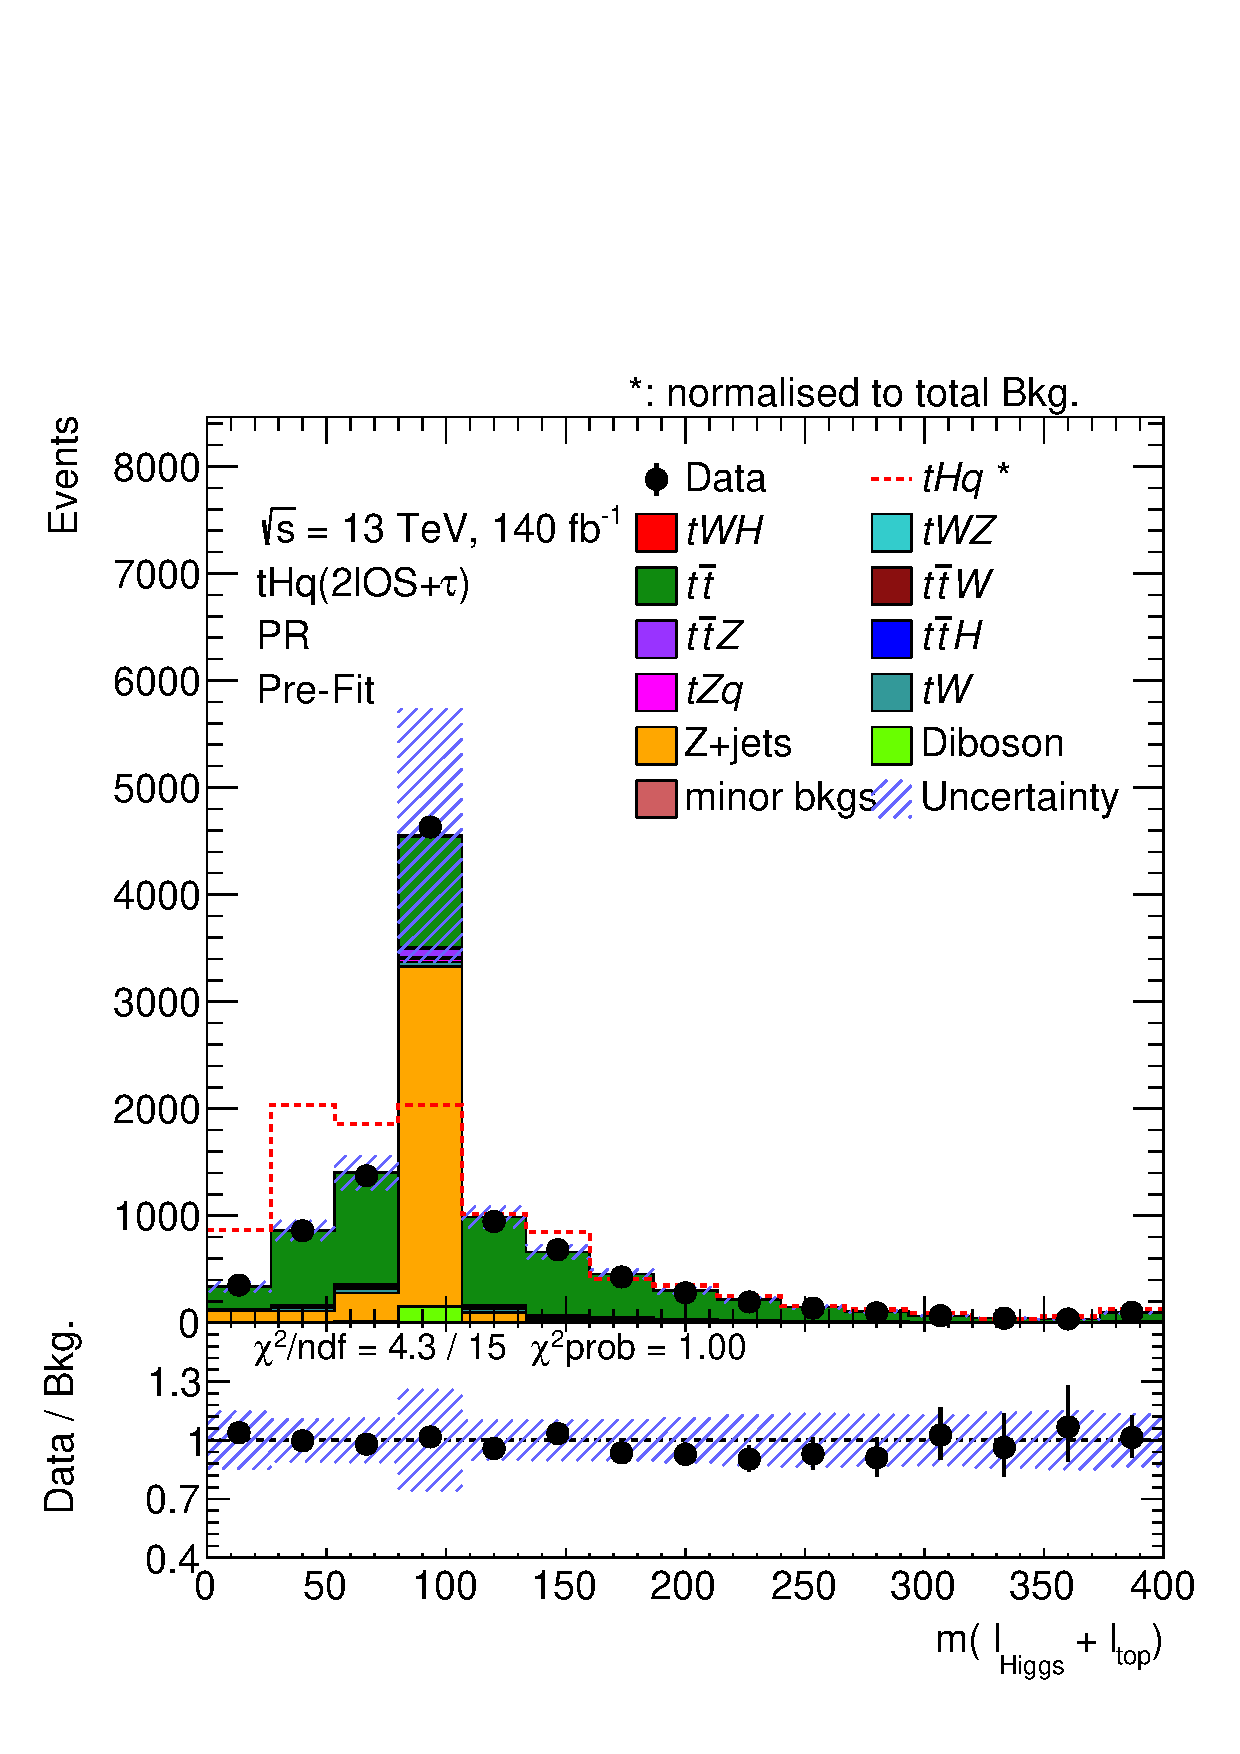
\includegraphics[width=\textwidth]{Chapter5_tHq/BDT_Results/BDT_Variables_ttbar_OS/a01_PR_lep_top_higgs_mass_2L1TAU_OS}
    \caption{La variable més rellevant de la BDT$(\ttbar|_{\text{OS}})$, la massa transversa dels dos leptons lleugers. }
     \label{fig:resum:EventSelection:BDT:VariablesRelevants:ttbarOS}
  \end{subfigure}
    \hfill
  \begin{subfigure}[b]{0.49\textwidth}
    \centering
    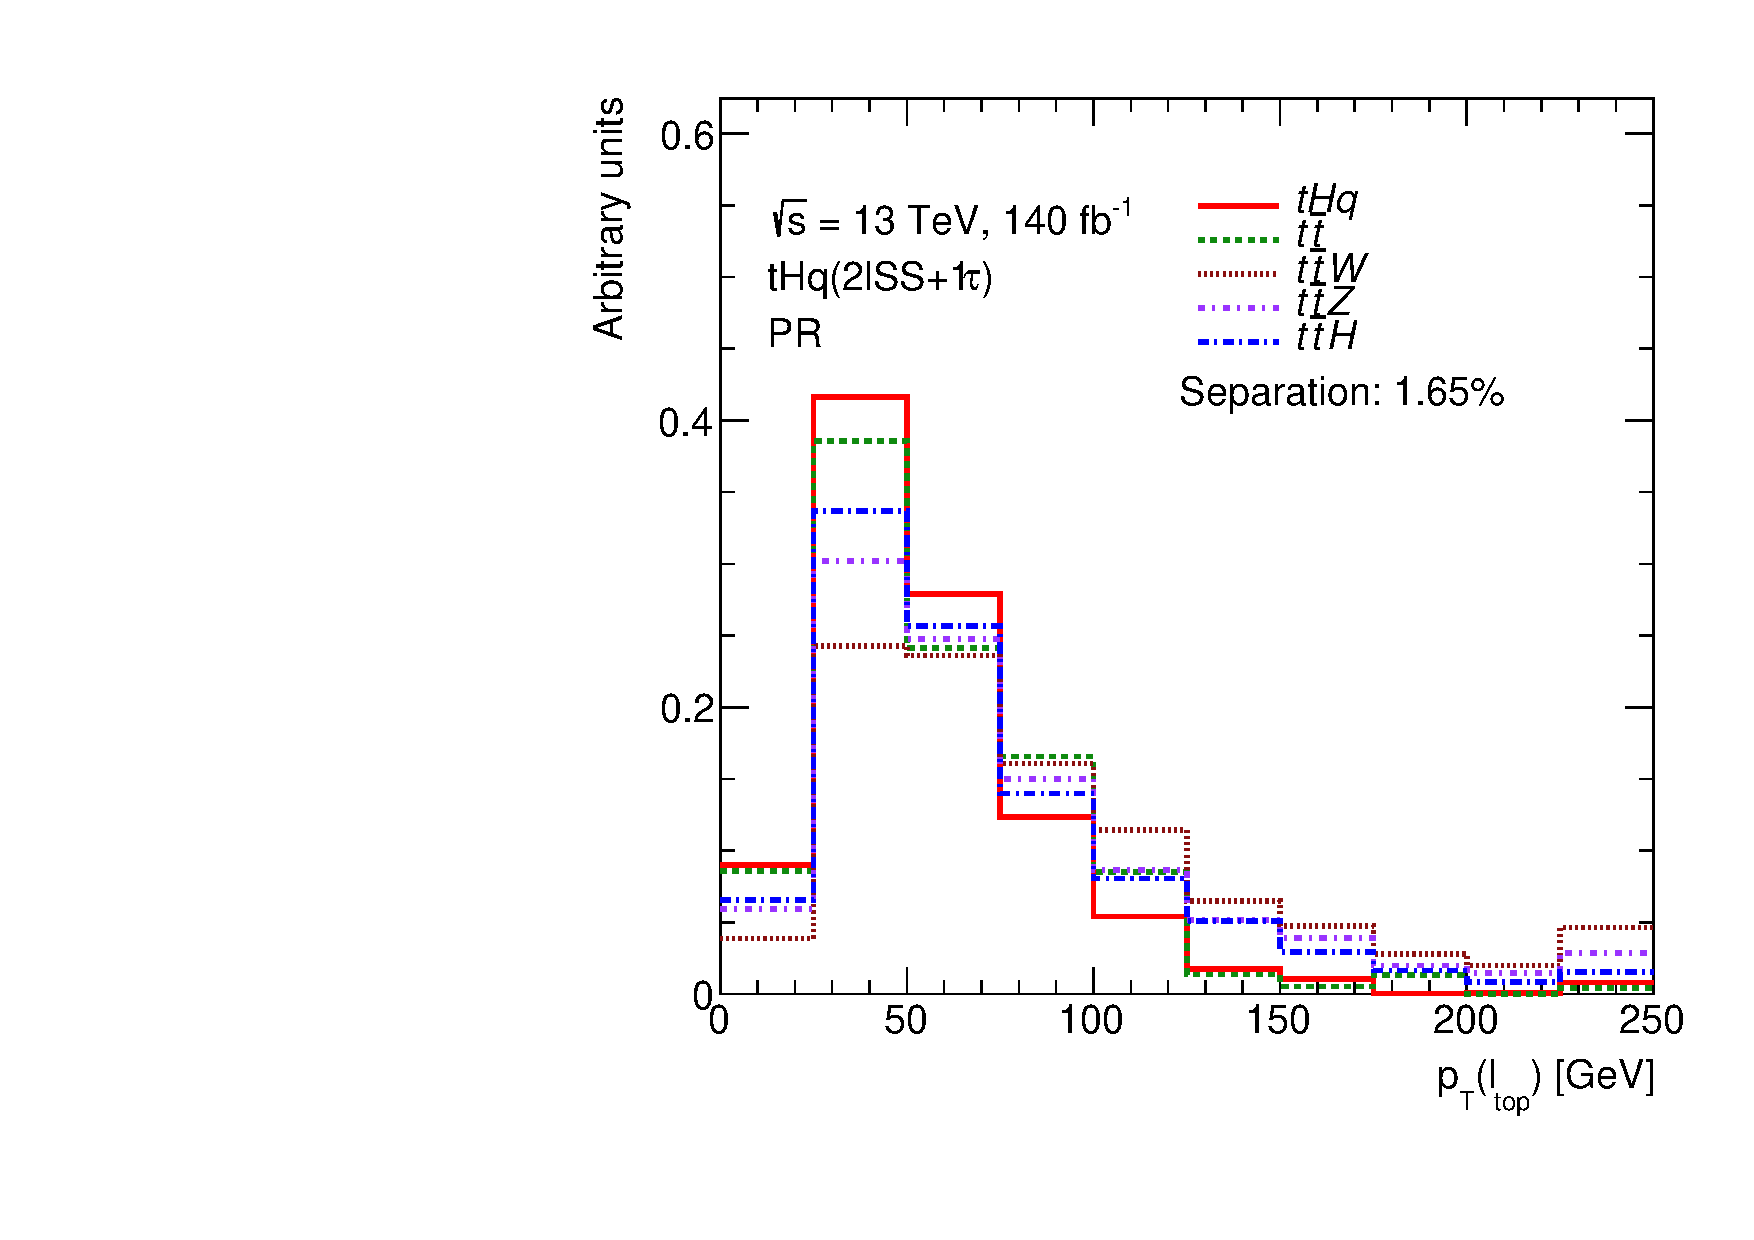
\includegraphics[width=\textwidth]{Chapter5_tHq/BDT_Results/BDT_Variables_tHq_SS/a03_PR_lepTop_pt_2L1TAU_SS}
    \caption{La variable més rellevant de la BDT$(\tHq|_{\text{SS}})$, el \pT del leptó lleuger del quark top.}
     \label{fig:resum:EventSelection:BDT:VariablesRelevants:tHqSS}
  \end{subfigure}
  \caption{Variables més rellevants per  cadascun dels tres models de classificació de processos: (a) BDT$(\tHq|_{\text{OS}})$, 
  	      (b) BDT$(\ttbar|_{\text{OS}})$ i (c) BDT$(\tHq|_{\text{SS}})$. Les bandes d'incertesa inclouen les incerteses estadístiques 
	      i sistemàtiques i el panell inferior presenta la relació entre les dades recollides i la simulació MC. Addicionalment, el 
	      $\chi^2$ mesura la concordança entre les dades reals i la mostra d'esdeveniments simulats per MC.} 
  \label{fig:resum:EventSelection:BDT:VariablesRelevants}
\end{figure}



Una vegada escollides les variables, cal optimitzar els hiperparàmetres de l'entrenament. Aquests s'encarreguen
de gestionar el procés d'aprenentatge del model, però no formen part d'ell i seleccionar els adequats és crucial, 
ja que pot influir significativament en el rendiment del model. L'optimització dels hiperparàmetres del BDT es fa utilitzant
un algoritme genètic~\cite{MitchellGA}. El conjunt òptim d'hiperparàmetres trobat es presenta per als tres
BDTs simultàniament a la Taula~\ref{tab:resum:BDT:Hyperparameters}.


\begin{table}[h]
\centering
\begin{tabular}{l|c|c|c}
\toprule
Hiperparàmetre 		& BDT$(\tHq|{\text{OS}})$ & BDT$(\ttbar|{\text{OS}})$ & BDT$(\tHq|_{\text{SS}})$ \\ \midrule
Profunditat màxima 		&  4 & 4 & 4 \\
Taxa d'aprenentatge 		& 0.1237 & 0.0334 & 0.04 \\
Nombre d'estimadors 	& 1500 & 1500 & 1500 \\
Pes mínim del fill 		& 0.52 & 0.077 & 0.026 \\
Escala de pesos positius 	& 268.838 & 0.36 & 83.21 \\
Estratègia de pes neg. 	& Només positius & Només positius & Valors absoluts \\ \bottomrule
\end{tabular}
\caption{Configuració dels hiperparàmetres utilitzats per a gestionar l'entrenament dels tres BDTs de 
gradient emprats per a la definició de regions. La resta d'hiperparàmetres es configuren amb els seus valors per defecte.}
\label{tab:resum:BDT:Hyperparameters}
\end{table}



El rendiment dels BDTs s'avalua a través de la corba de característiques operatives del 
receptor (ROC). Per a un model de classificació binària, la corba ROC representa la relació 
entre la taxa de veritables positius (sensibilitat) i la taxa de falsos positius (1 - especificitat) 
per a diferents llindars de decisió. 
Les corbes ROC dels tres BDTs de definició de regió es presenten a la Figura~\ref{fig:resum:BDT:ROC_Curves}. 
L'àrea sota la corba ROC (AUC per les seues sigles en anglés) és un altre indicador del rendiment del model: un valor d'AUC 
proper a 1 indica un model molt precís, mentre que un valor d'AUC proper a 0,5 indica un 
rendiment no millor que l'atzar. Per als models BDT$(\tHq|_{\text{OS}})$, BDT$(\ttbar|_{\text{OS}})$ i BDT$(\tHq|_{\text{SS}})$,
les AUC són, respectivament $0.637\pm0.004$, $0.730 \pm 0.003$ i $0.6706 \pm0.0013$.


\begin{figure}[h]
  \centering  
  \begin{subfigure}[b]{0.31\textwidth}
    \centering
    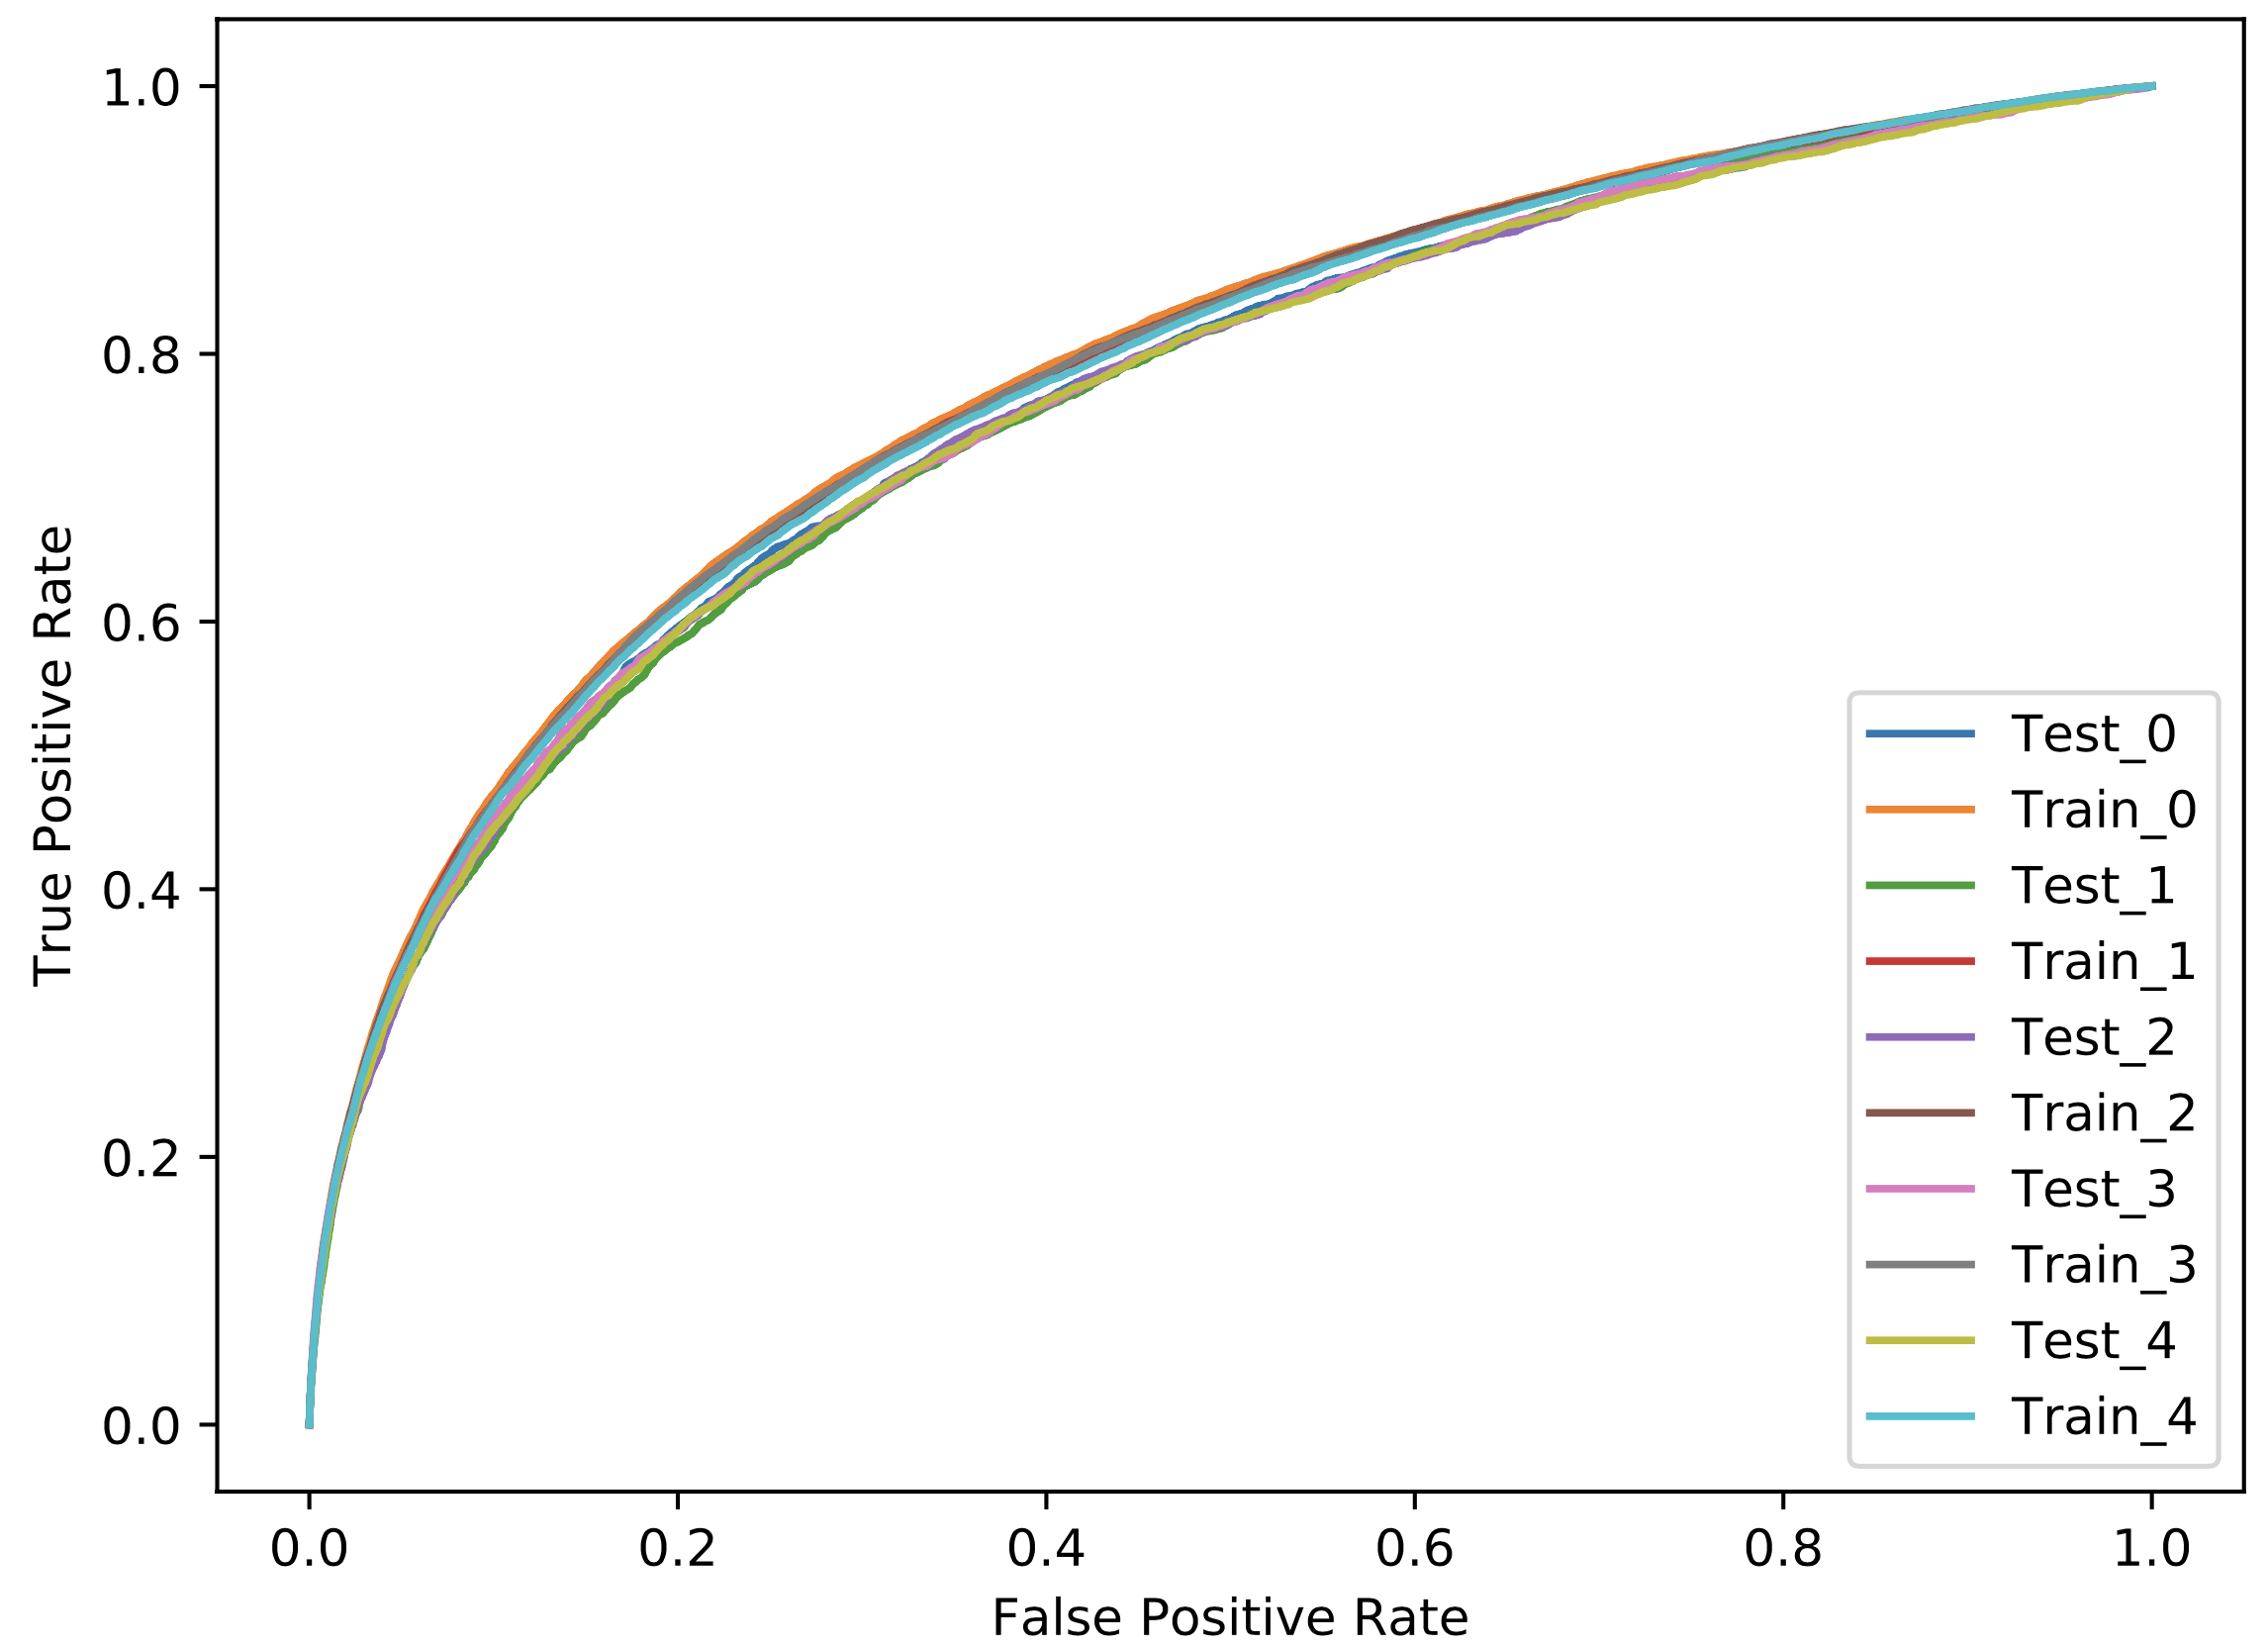
\includegraphics[width=\textwidth]{Chapter5_tHq/BDT_Results/ROC_curve_tHq_OS_LowRes}
    \caption{BDT$(\tHq|_{\text{OS}})$}
     \label{fig:resum:BDT:ROC_Curves:tHqOS}
  \end{subfigure}
  \hfill
  \begin{subfigure}[b]{0.31\textwidth}
    \centering
    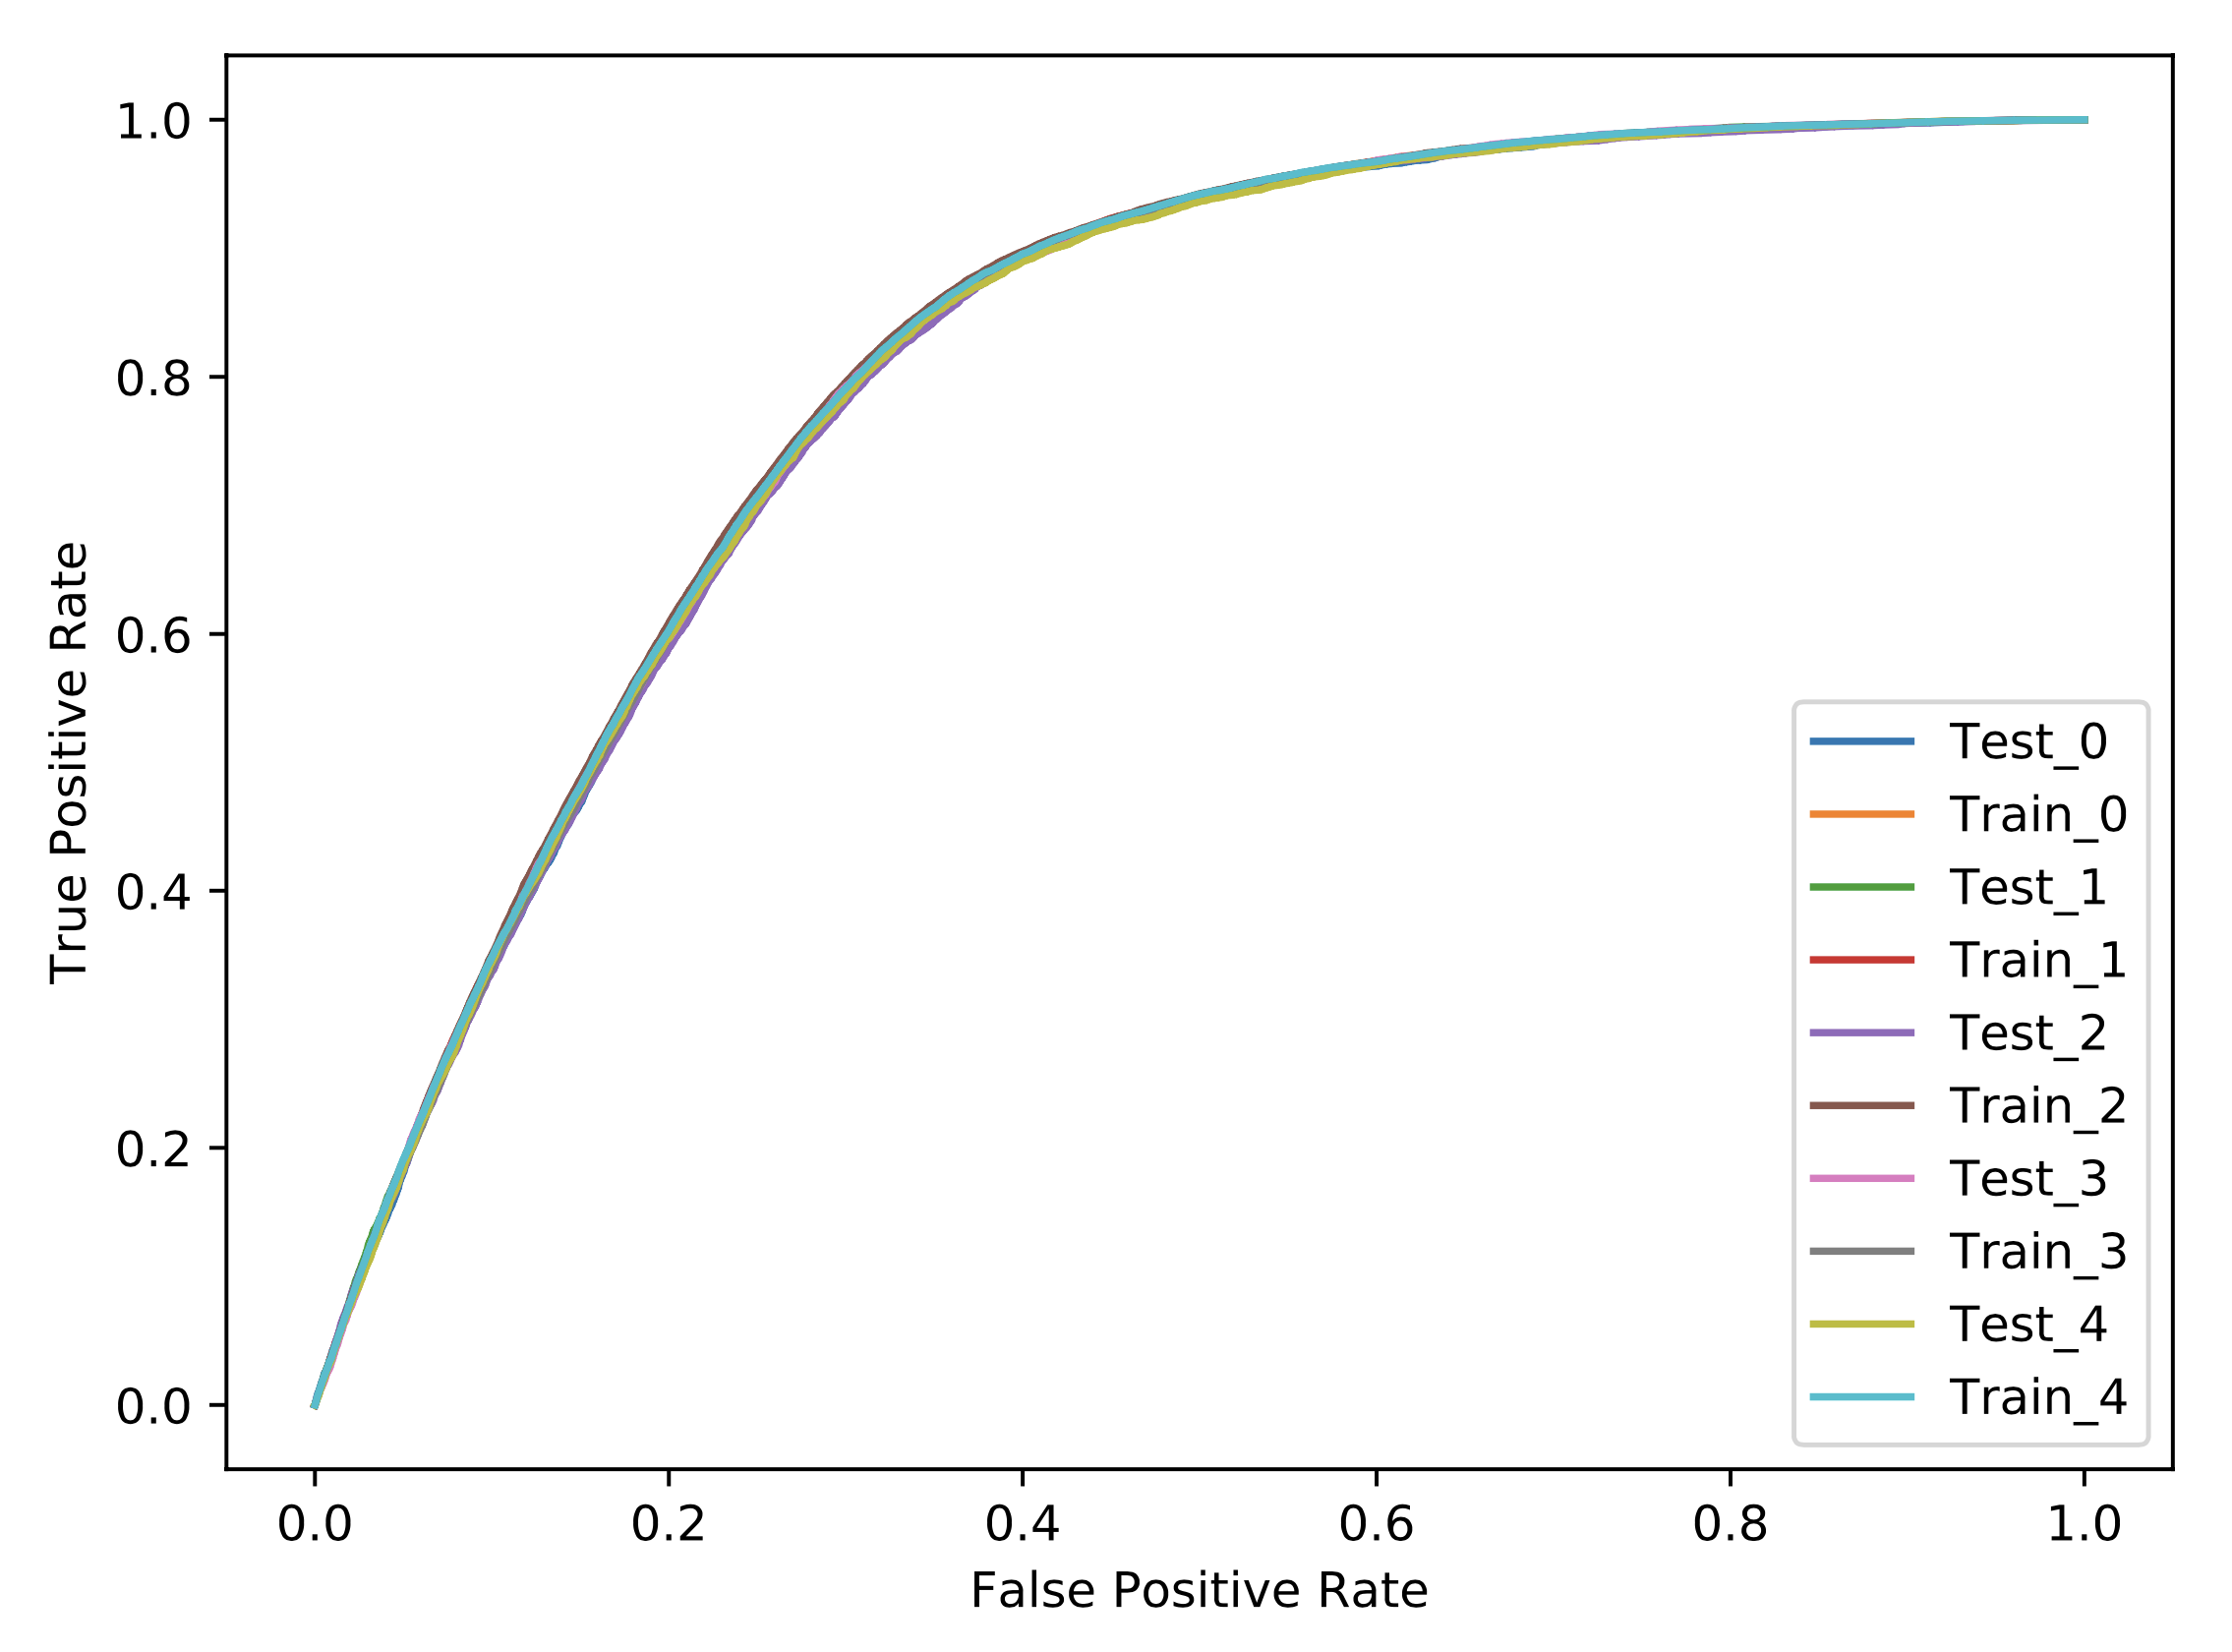
\includegraphics[width=\textwidth]{Chapter5_tHq/BDT_Results/ROC_curve_ttbar_OS_LowRes}
    \caption{BDT$(\ttbar|_{\text{OS}})$}
     \label{fig:resum:BDT:ROC_Curves:ttbarOS}
  \end{subfigure}
    \hfill
  \begin{subfigure}[b]{0.31\textwidth}
    \centering
    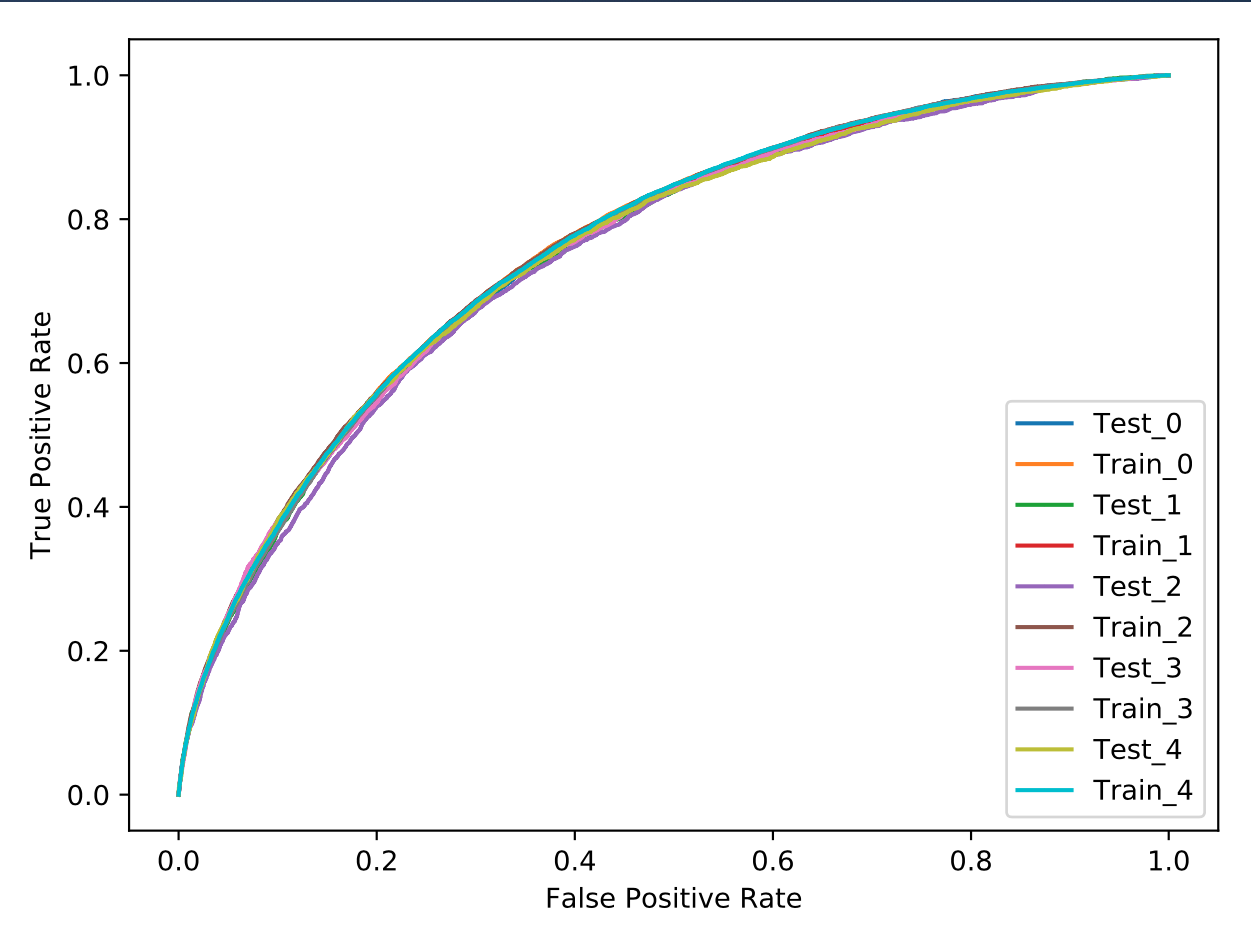
\includegraphics[width=\textwidth]{Chapter5_tHq/BDT_Results/ROC_curve_tHq_SS_LowRes}
    \caption{BDT$(\tHq|_{\text{SS}})$}
     \label{fig:resum:BDT:ROC_Curves:tHqSS}
  \end{subfigure}
  \caption{ROC per a tots els grups dels tres models BDT. En cada figura es poden veure cinc parelles de 
  	       corbes ROC. Cada parella correspon a un grup i, dins d'un grup, la parella tracta les mostres 
	       d'entrenament i de prova separadament.}
  \label{fig:resum:BDT:ROC_Curves}
\end{figure}

La distribució de les BDTs en funció del \textit{fold} es mostra a la Figura~\ref{fig:resum:BDT:OS_ScoresCombo}.
En aquesta figura també es mostren les fraccions entre els esdeveniments de cada \textit{fold} i es pot apreciar 
clarament com tots cinc són perfectament compatibles entre si. Açò vol dir que el model té bona capacitat per a 
generalitzar.


\begin{figure}[h]
  \centering  
  \begin{subfigure}[b]{0.31\textwidth}
    \centering
    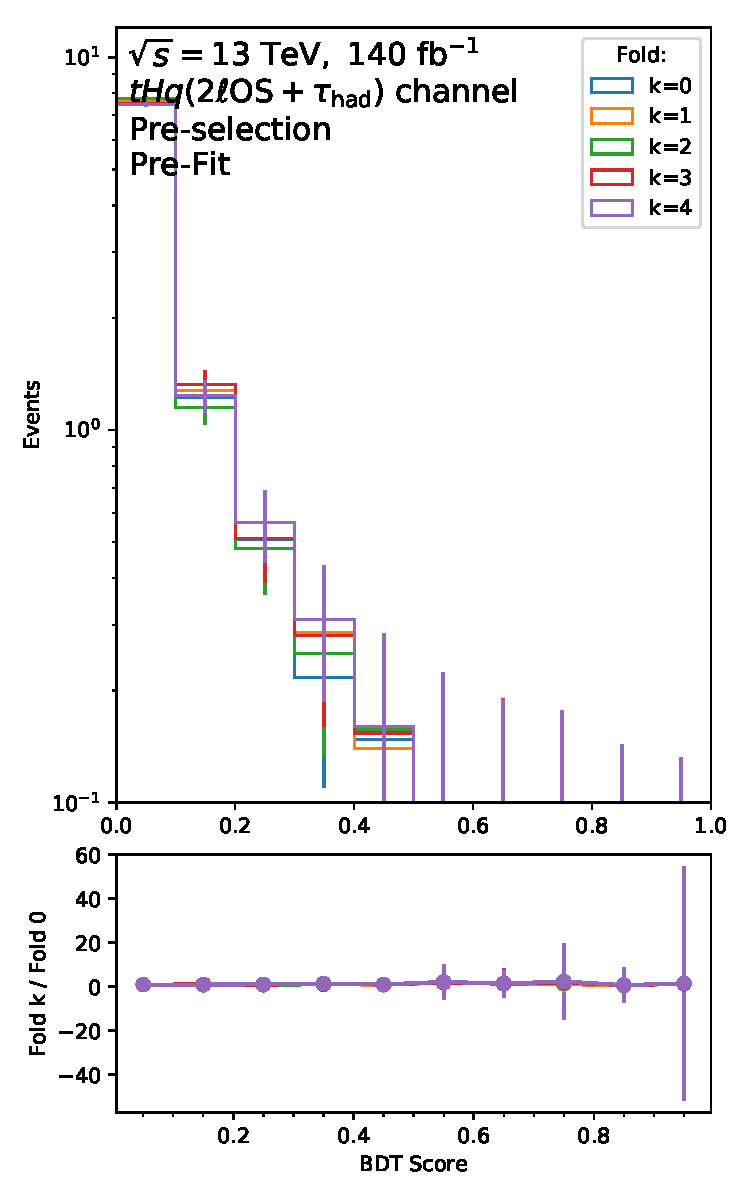
\includegraphics[width=\textwidth]{Chapter5_tHq/BDT_Results/test_fold_tHq_2L_with_ratio_OS_tHq}
    \caption{BDT$(\tHq|_{\text{OS}})$}
     \label{fig:resum:OS_ScoresCombo:tHq}
  \end{subfigure}
  \hfill
  \begin{subfigure}[b]{0.31\textwidth}
    \centering
    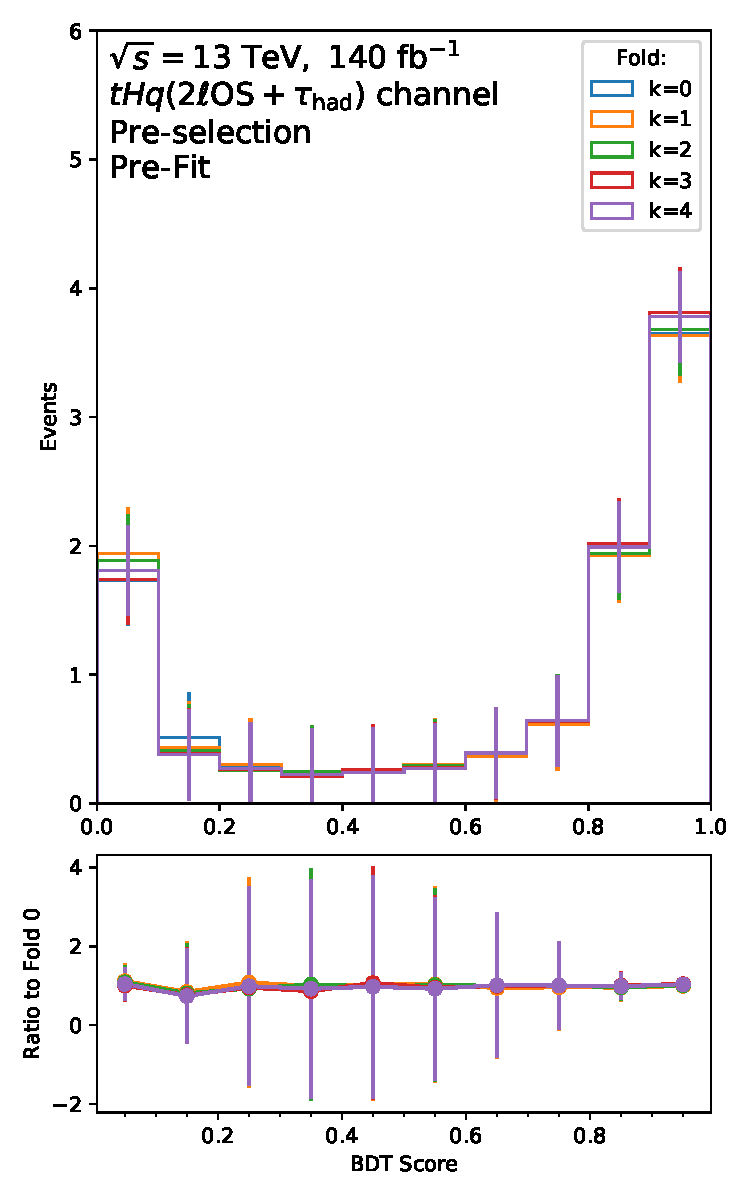
\includegraphics[width=\textwidth]{Chapter5_tHq/BDT_Results/test_fold_tHq_2L_with_ratio_OS_ttbar}
    \caption{BDT$(\ttbar|_{\text{OS}})$}
     \label{fig:resum:BDT:OS_ScoresCombo_ttbar}
  \end{subfigure}
    \hfill
  \begin{subfigure}[b]{0.31\textwidth}
    \centering
    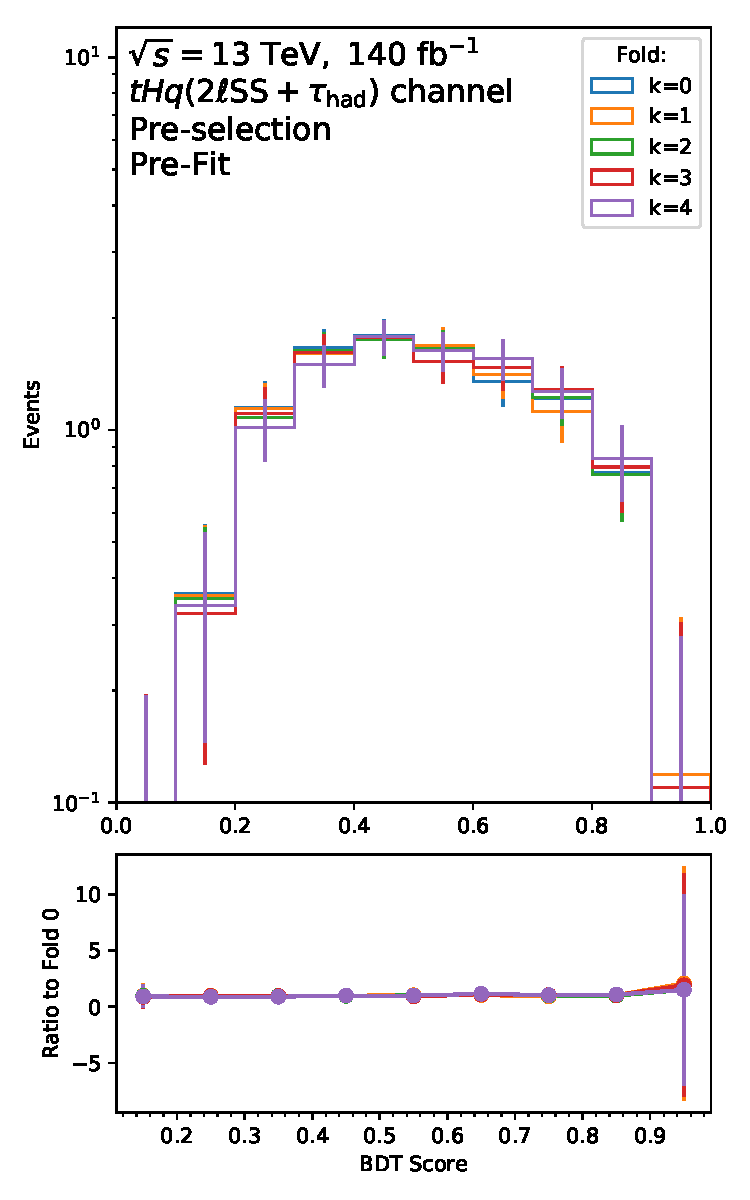
\includegraphics[width=\textwidth]{Chapter5_tHq/BDT_Results/test_fold_tHq_2L_with_ratio_SS_tHq}
    \caption{BDT$(\tHq|_{\text{SS}})$}
     \label{fig:resum:BDT:SS_ScoresCombo_tHq}
  \end{subfigure}
  \caption{En el panell superior de cada figura, es mostra el perfil del BDT per als cinc \textit{folds} simultàniament. 
  L'error en cada bin del panell superior correspon a la desviació estàndard. En el panell inferior, es presenta la la fracció 
  d'esdeveniments entre el primer grup (Grup 0) i tots els altres. Ambdós panells comparteixen el mateix eix x. Per a tots 
  els \textit{folds} dins d'un BDT, les distribucions són compatibles dins de l'error estadístic. Això indica que el model 
  generalitza adequadament i no es veu afectat pel conjunt específic d'esdeveniments que s'utilitzen per a l'entrenament 
  en cada grup. Els perfils mostrats són dibuixats emprant només les mostres de test.}
  \label{fig:resum:BDT:OS_ScoresCombo}
\end{figure}



\FloatBarrier
%%%%%%%%%%%%%%%
%         Fons d'indertesa        %
%%%%%%%%%%%%%%%
\subsection{Fonts d’incertesa}
\label{sec:resum:Incerteses}
La incertesa en física es refereix al fet que és impossible mesurar qualsevol quantitat física amb precisió perfecta. 
Això es deu al fet que tots els instruments de mesura tenen limitacions i estan subjectes a diverses fonts d'error.
Aquestes incerteses proporcionen una mesura de l'interval dins del qual es preveu que es trobe el valor real d'una 
quantitat mesurada. Hi ha dos tipus principals d'incerteses: la incertesa estadística i la incertesa sistemàtica.

La incertesa estadística sorgeix de l'atzar inherent o fluctuacions en les dades finites. Aquestes fluctuacions són 
típicament descrites per mètodes estadístics, com les distribucions de probabilitat, i són quantificades per mesures 
estadístiques com la desviació estàndard o intervals de confiança. Les incerteses estadístiques són completament 
no correlacionades entre mesures successives, la qual cosa significa que cada mesura porta la seua pròpia incertesa 
estadística independent.

D'altra banda, les incerteses sistemàtiques engloben totes les fonts d'error o variació que no són directament degudes 
a l'estadística de les dades. Les incerteses sistemàtiques poden ocórrer en qualsevol punt de la cadena d'anàlisi. 
Estan associades amb diversos factors, incloent-hi l'aparell de mesura, les condicions experimentals, les suposicions 
fetes en l'anàlisi, els models teòrics emprats, la reconstrucció d'objectes, les tècniques d'estimació del fons i les 
simulacions MC, entre molts altres. Les incerteses sistemàtiques són completament correlacionades entre mesures 
successives, la qual cosa significa que afecten consistentment tot el conjunt de dades.

Les incerteses sistemàtiques es classifiquen en dos grans grups depenent del seu origen: incerteses teòriques 
i incerteses experimentals.



\subsubsection{Incerteses teòriques}
\label{sec:resum:Incerteses:teo}

Aquestes es refereixen a la modelització a simulació de MC i el coneixement teòric sobre els diferents processos.
Per a quantificar aquestes incerteses, es comparen diferents prediccions teòriques i variacions en els paràmetres 
del model de MC per a avaluar el seu impacte en els resultats. Les variacions són comparades amb el mètode 
principal (referit com a \textit{nominal}), la qual cosa, permet estimar l'exactitud i la fiabilitat dels càlculs teòrics.

Les incerteses de modelatge s'avaluen de tres maneres: comparant la predicció del generador de MC nominal 
amb la de generadors alternatiu, variant els paràmetres interns de la simulació nominal o variant la secció transversal 
predita dins de la incertesa teòrica. 

\subsubsection{Incerteses experimentals}
\label{sec:resum:Incerteses:exp}
Les incerteses experimentals juguen un paper crucial en els experiments de física de partícules, ja que sorgeixen del
mateix procés de mesura. En el context de les anàlisis de ATLAS, aquestes incerteses provenen principalment de 
factors relacionats amb el detector i abasten diversos aspectes, com les limitacions de l'aparell de mesura, els
procediments de calibració i l'eficàcia de reconstruir objectes físics dins del detector. Algunes fonts comunes d'incerteses 
experimentals inclouen:
\begin{itemize}
	\item \textbf{Luminositat}: Per a cada any de presa de dades, hi ha una incertesa en la luminositat integrada 
	recollida pel detector ATLAS.
	
	\item \textbf{Reponderació de Pile-up}: Els esdeveniments de les mostres de simulació MC es reponderen 
	per a coincidir amb la distribució observada del nombre mitjà d'interaccions per creuament de feixos 
	en les dades~\cite{Marshall:2014mza}. El valor d'aquesta incertesa s'obté reescalant el valor de <$\mu$> 
	en les dades per  $1/0.99$ i $1/1.07$ al voltant del factor d'escala nominal de $1/1.03$~\cite{Buttinger:2014726}.
	
	\item \textbf{Escala d'energia del jet}: La calibració de l'escala d'energia del jet (JES) corretgeix l'energia i la direcció 
	dels jets per a coincidir amb la dels jets reconstruïts a nivell de partons~\cite{ATLAS:2020cli}. 
	La incertesa associada amb JES s'obté de dades de feix de prova, dades de col·lisions LHC
	i simulacions MC.

	\item \textbf{Resolució d'energia del jet}: La resolució d'energia del jet (JER) es refereix a la capacitat de l'experiment per 
	a mesurar l'energia dels jets. La JER es mesura per separat per a dades i MC utilitzant les dues tècniques in-situ
	descrites en les referències~\cite{ATLAS:2020cli, ATLAS:2017bje}. %Una incertesa de JER es  defineix com la diferència 
	%quadràtica entre la JER per a dades i MC~\cite{jetEtMissRecommendations}.
	
	\item \textbf{Jet vertex tagger}: Les incerteses associades amb l'identificador de vèrtexs provenen de la contaminació 
	residual de jets de pile-up~\cite{ATLAS-CONF-2014-018, ATLAS:2017ywy}.

	\item \textbf{\tauhad mal identificat}: Les incerteses sistemàtiques associades amb les identificacions de \tauhad 
	depenen del punt de treball triat a la RNN que s'encarrega de la identificació dels \tauhad.%presentada a la Taula~\ref{tab:Resum:ObjectDefReco:Tau}.


	\item \textbf{Taxa de \tauhad mal identificat}: Per a abordar la incertesa associada amb el mètode
	de determinació de les probabilitats de \tauhad mal identificat, el mètode de l'ajust de plantilla es
	compara amb el mètode de recompte. Ambdós mètodes són descrits a la Secció~\ref{chap:resumen_val:tHq:Fons}.
	
	\item \textbf{Etiquetatge de sabors pesats i lleugers}: L'eficiència de l'algoritme d'etiquetatge de sabors es
	mesura per a cada sabor de jet utilitzant mostres de control de dades i simulació. Aquesta avaluació
	dóna factors de correcció per a ajustar les taxes d'etiquetatge en les simulacions. 
	
	\item \textbf{Eficiència d'Electrons}: S'utilitza un mètode específic per corregir diferències en l'eficiència 
	de reconstrucció d'electrons entre dades reals i simulades. Això es mesura en certes classes d'esdeveniments de partícules.

	\item \textbf{Eficiència de Muons}: De forma anàloga als electrons, es realitzen correccions per ajustar les eficiències
	d'identificació i aïllament dels muons, basades en diferents tipus d'esdeveniments.

	\item \textbf{Escala d'Energia i Resolució d'Electrons}: Es corregissen petites discrepàncies entre les simulacions i 
	les dades reals respecte a l'energia i la resolució dels electrons.

	\item \textbf{Escala de Moment i Resolució de Muons}: Es fan ajustos en les simulacions dels muons per alinear-les amb
	les observacions reals, enfocant-se en la seua escala de moment i resolució.

	\item \textbf{Terme Suau de \MET}: S'apliquen correccions a l'escala i la resolució d'una part específica de la mesura 
	\met, que no està associada amb objectes calibrats.	
\end{itemize}


%%%%%%%%%%%%%%%
%        Resultats del fit        %
%%%%%%%%%%%%%%%
\subsection{Resultats}
\label{sec:resum:Resultats}


%%%%%%%%%%%%%
%        Fit :: mètode        %
%%%%%%%%%%%%%
\subsubsection{Mètode de l'ajust de màxima versemblança}
\label{sec:resum:Resultats:Fit}
La tècnica utilitzada per mesurar la normalització del senyal ($\mu_{\tHq}^{\dileptau}$) i del processos de fons que es desitgen
controlar ($k_p$) és coneguda com a \textit{mètode de l'ajust de màxima versemblança}, encara que és més habitual referir-se a aquesta pel
seu nom en anglés \textit{maximum likelihood fit}.  El $\mu$ i $k_p$ s'anomenen conjuntament com \textit{paràmetres d'interés del sistema} (POI).  
El factor de normalització del senyal és també conegut com força del senyal i es defnineix com:
\begin{equation*}
	\mu_{\tHq} =\frac{\sigma^{\text{obs}}}{\sigma^{\text{pred}}}\,.
\end{equation*}
El mètode de màxima versemblança és àmpliament utilitzat als anàlisis d'ATLAS, hem d'estimar desenes o fins i 
tot centenars de fonts sistemàtiques d'incertesa. Aquestes incerteses són intruïdes a l'ajust de versemblança 
mitjançant uns paràmetres al model anomenats \textit{paràmetres de molèstia} (NPs). %L'objectiu del NPs és 
%cobrir els 

Aquest mètode funciona maximitzant la funció de versemblança per distribucions en diagrames de 
barres\footnote{Cada barra del diagrama de barres és anomenada \textit{bin} i al diagrama en si ens referim com a \textit{histograma}.}:
\begin{align}\label{eq:Resum:ChaptH:BinnedFit}
\begin{split}
	L(\overrightarrow{n}|\mu, \overrightarrow{\theta}) 
	& = \prod_{i \in \text{bins}} \mathcal{P}\left(n_{i}^{\text{obs}} | \mu \cdot s_{i}^{\text{exp}}(\overrightarrow{\theta}) + b_{i}^{\text{exp}}(\overrightarrow{\theta})\right) \\
	& \times \prod_{j \in \text{syst}} \mathcal{G}(\theta_{0, j}|\theta_{j}, \Delta \theta_{j}) 
	\times \prod_{s \in \gamma} \mathcal{P}(\theta_{0, s}|\theta_{s}, \Delta \theta_{s}) \, .
\end{split}
\end{align}
Ací, l'índex $i$ es refereix al bins dels histogrames que s'utilitzen al fit. L'índex $j$ 
corre sobre els NPs que es refereixen a les fonts d'incertesa sistemàtica i l'índex 
$s$ als NPs associats amb la incertesa estadística de la mostra de simulacions 
de MC (anomenades \textit{gammas} o $\gamma$). 
$\mathcal{P}$ i $\mathcal{G}$ són, respectivament, les funcions de les distribucions
Poissonianes i Gaussianes.  El nombre d'esdeveniments observat és $n_{i}^{\text{obs}}$
i l'esperat $n_{i}^{\text{exp}}$, que es calcula:
\begin{equation*}
	n_{i}^{\text{exp}} = \mu \cdot s_{i}^{\text{exp}}(\overrightarrow{\theta}) + \sum_{p \in \text{Bkg}} k_{p} \cdot b_{i}^{\text{exp}}(\overrightarrow{\theta}) \, ,
\end{equation*}
on $\mu$ i $k_p$ són les normalitzacions de la senyal i els diferents fons. 
A l'equació~\ref{eq:Resum:ChaptH:BinnedFit}, els $\theta$ son els NPs, mentre
que $\theta_{0}$ i $\Delta \theta$ són el valor nominal del NP i la variació d'una desviació 
estàndard aplicada per valorar el seu impacte.



% Upper limit
A més del factor de normalització del senyal, també es proporciona un límit superior mitjançant una prova estadística. 
La prova depén del valor de $\mu$, i el límit superior s'extreu utilitzant el mètode descrit a la 
referència~\cite{Read:2002hq} per a establir un nivell de confiança del 95\%. 
La interpretació de $\mu$, així com el límit superior, també pot ser escrita en termes de la secció eficaç 
de producció del procés de senyal de la següent manera:
\begin{equation}
	\sigma^{\text{obs}} = \mu(\tHq) \times \sigma^{\text{pred}} \, ,
\end{equation}
on $\sigma^{\text{pred}}$ és el valor de la secció de producció predit per la teoria.


%%%%%%%%%%%%%%%
%        Fit :: Estratègia         %
%%%%%%%%%%%%%%%
\subsubsection{Estratègia d'ajust}

\paragraph{Experiment cec}\mbox{}\\
A l'hora de formular l'estratègia de l'anàlisi és crucial evitar examinar les regions de dades
que es preveu que tinguen una alta concentració d'esdeveniments de senyal \tHq.
Aquesta pràctica de cegar l'experiment s'anomena \textit{blinding} i juga un paper
fonamental a l'hora de protegir l'anàlisi de potencials biaix o predisposicions
que podrien ocórrer si els investigadors es veuen influenciats per variacions estadístiques observades.

En aquesta recerca, el punt corresponent a les dades en un bin només es mostrat si la fracció de 
senyal esperada era menor que 0.3\% i tots els bins en les SRs estaven completament cegats. 
Només en la Secció~\ref{sec:resum:Resultats:FullFit} la
recerca es fa amb dades des-cegades. 

\paragraph{Tipus d'ajust}\mbox{}\\
Primerament, fem un ajust utilitzant únicament les mostres de simulacions de MC. En aquest
ajust cap dada real és emprada. Aquesta configuració es coneix com a hipòtesis d'Asimov.
Els resultats d'aquesta mena d'ajust es presenten a la Secció~\ref{sec:resum:Resultats:Asimov}.
El propòsit d'aquesta mena d'ajust és avaluar la sensitivitat de l'anàlisi i comprovar l'estabilitat de 
l'ajust amb la configuració escollida. Si l'ajust d'Asimov presenta cap mena d'inestabilitat podem 
canviar la definició de les regions fetes servir a l'ajust o els paràmetres que deixem flotar als càlculs.

Si l'ajust d'Asimov no funciona correctament, les dades reals són parcialment influïdes als càlculs. 
Primer a les regions de control, on fem unajust per a mesurar la normalització del fons que desitgem 
controlar ($k_{p}$). Per fer això assumim la hipòtesis de senyal nul·la (és a dir, $\mu_{\tHq}$=0). 
Aquesta configuració coneix com ajust de les CR fons únicament.

Després les dades s'utilitzen a totes les regions de l'anàlisi amb la hipòtesi nul·la i, de nou, es calculen el $k_{p}$. 
La diferència ací és que podem determinar l'impacte de la SR en la determinació dels factors de normalització. 
Encara que la SR s'utilitza en aquest ajust, a les gràfiques continua cegada per a no produir cap biaix.
Per simplicitat, els resultats d'aquests dos tipus d'ajust no estan inclosos en el resum. 

Finalment, si tots els ajustos preliminars funcionen correctament. L'ajust de màxima versemblança per a 
distribucions amb bins es realitza emprant totes les regions i tenint també en compte el MC del senyal. 
Aquest ajust final es du a terme amb dades des-cegades. Els resultats de l'ajust final es presenten a la 
Secció~\ref{sec:resum:Resultats:FullFit}.

\paragraph{Poda de the NPs}\mbox{}\\
En principi, introduïm un NP per a cada incertesa sistemàtica en la funció de versemblança.
A causa del gran nombre de paràmetres d'ajust, aquesta tècnica és molt costosa computacionalment
i pot trigar hores o dies per fer un sol ajust.
El que ens preocupa és quines fonts sistemàtiques tenen una gran contribució a la
incertesa dels POI.  Si identifiquem les fonts d'incertesa que no tenen una contribució significativa,
podem llevar-les de l'ajust i agilitzar el procés. Aquesta tècnica és referida com a \textit{poda}. 

\paragraph{Configuracions de l'ajust de màxima versemblança}\mbox{}\\
En aquest cas, per configuracions, ens referim a quines regions de l'espai de fases
incloem en l'ajust de màxima versemblança i a quins factors de normalització deixem
flotar com a paràmetres lliures. Les diverses estratègies que sigut explorades es presenten
a la Taula~\ref{tab:resum:FitConfiguration:OS} per al canal \dilepOStau i a la
Taula~\ref{tab:resum:FitConfiguration:SS} per al \dilepSStau.

\begin{table}[h]
\centering
\begin{tabular}{l|c|c|c}
\toprule
& \ttbar i \Zjets & Paràmetres lliures & Pesos corregits \\
\midrule
Utilitzat & CR & $\mu_{\tHq}$ , $k_{\ttbar}$, $k_{\Zjets}$ & \checkmark \\
Alternativa 1 & VR & $\mu_{\tHq}$ & \checkmark \\
%Alternativa 2 & VR & $\mu_{\tHq}$ , $k$(\ttbar), $k$(\Zjets) & \checkmark \\
Alternativa 2 & CR & $\mu_{\tHq}$ & \checkmark \\
Alternativa 3 & CR & $\mu_{\tHq}$ , $k_{\ttbar}$, $k_{\Zjets}$ & \xmark \\
\bottomrule
\end{tabular}
\caption{Diferents configuracions d'ajust de versemblança provades per al canal \dilepOStau.
La columna ``\ttbar i \Zjets'' indica si les regions de l'esapi de fases dedicades a aquests dos processos
són utilitzades als càlculs (CR) i si només s'utilitzen per a la validació de l'ajust (VR).
Totes aquestes configuracions han estat explorades (amb dades cegues) per a comprovar
l'impacte de cada opció als resultats.}
\label{tab:resum:FitConfiguration:OS}
\end{table}


\begin{table}[h]
\centering
\begin{tabular}{l|l|c}
\toprule
		 	& CRs & $k_{p}$ lliures \\ \midrule
Utilitzat 		& Tots els fons & $k_{\ttbar, \ttX}$ \\ 
Alternativa 1 	& \ttbar, \ttX & $k_{\ttbar}$, $k_{\ttW}$ \\
Alternativa 2	& \ttbar, \ttX & $k_{\ttbar}$, $k_{\ttX}$ \\
Alternativa 3& \ttbar, \ttX & $k_{\ttbar}$, $k_{\ttW}$, $k_{\ttH}$, $k_{\ttZ}$ \\

\bottomrule
\end{tabular}
\caption{Diferents configuracions de l'ajust provades per al canal \dilepSStau.
La columna CR fa referència a quines regions de control s'utilitzen a l'ajust i
la columna $k_{p}$ lliures es refereix a quins factors de normalització es calculen juntament amb la $\mu_{\tHq}^{\dilepSStau}$.
Totes aquestes han estat explorades amb dades cegues per a comprovar com la configuració influencia els resultats.}
\label{tab:resum:FitConfiguration:SS}
\end{table}
 
 
Com es pot veure a l'última columna de la Taula~\ref{tab:resum:FitConfiguration:OS}, pel canal \dilepOStau s'ha 
explorat no utilitzar els factors d'escala que corregeixen les imprecisions en l'estimació del fons a causa d'objectes 
físics erròniament identificats\footnote{Principalment quarks o gluons mal identificats com a \tauhad.}. La idea 
consisteix en controlar la freqüència d'aquesta mena de processos fent ús dels factors de normalització $k_{\ttbar}$
i $k_{\Zjets}$. Els resultats preliminars amb aquesta opció no eren massa prometedors.
Finalment, s'ha fet servir la configuració en la que $k_{\ttbar}$i $k_{\Zjets}$ són calculats. Encara que es podria pensar 
que no cal controlar \ttbar i \Zjets perque ja disposem dels factors d'escala que corregissen\footnote{En aquest context corregir significa fer que el MC represente correctament la física d'ATLAS, incloent-hi el nombre d'esdeveniments de processos mal identificats.} la quantitat 
d'esdeveniments de MC que tenim d'aquest tipus, la realitat és que l'ajust millora quan $k_{\ttbar}$i $k_{\Zjets}$  són paràmetres lliures del sistema.
 

Pel que respecta al canal \dilepSStau, el principal problema que hi ha és que hi ha un excés generalitzat 
d'esdeveniments de simulats amb MC respecte a les dades recol·lectades i això provoca que l'ajust siga 
prou inestable quan tracta de controlar els processos de fons. Inicialment, s'ha tractat de controlar $k_{\ttbar}$ 
i $k_{\ttW}$ fent servir una regió dedicada per a \ttbar i una altra per a \ttX\footnote{Cal notar que és 
complicat discriminar entre \ttW, \ttZ i \ttH.}. El motiu per tractar de fitar \ttW en comptes de \ttX és que hi ha 
una lleugera tensió entre les prediccions teòriques sobre la producció de \ttW i els resultats experimentals. 
Tant ATLAS com CMS han mostrat certa sobreabundància en les dades en comparació amb les prediccions 
teòriques~\cite{ATLAS:2023gon, CMS:2022tkv}. En qualsevol cas, ajustar únicament \ttW i \ttbar no és suficient 
per a corregir el modelatge. Si tractem de controlar els \ttbar, \ttW, \ttZ i \ttH de forma independent, el fit resulta 
molt inestable perquè són massa paràmetres lliures per a una mostra estadística insuficient.
Llavors, els dos plantejaments amb millors resultats per al canal \dilepSStau són o bé ajustar $k_{\ttbar}$ i 
$k_{\ttX}$ en les dues regions que tenim, o bé juntar tots els fons en una sola regió ortogonal al SR i obtindre un 
únic factor de normalització, $k_{\ttbar, \ttX}$.



%%%%%%%%%%%%%%%
%        Fit :: ASIMOV        %
%%%%%%%%%%%%%%%
\subsubsection{Ajust d'Asimov}
\label{sec:resum:Resultats:Asimov}
L'ajust Asimov consisteix a utilitzar només els esdeveniments generats per MC com si aquests fossin 
les dades recollides. Les dades Asimov es construeixen com a conjunts de dades distribuides en bins, 
en els quals el $n_{i}^{\text{obs}}$ de cada bin es fixa a $n_{i}^{\text{exp}}$. 
Sota la hipòtesi Asimov, la força del senyal en l'Equació~\ref{eq:Resum:ChaptH:BinnedFit} es fixa a la unitat. 
En aquesta mateixa expressió, els diferents NPs es fixen als seus valors nominals ($\theta = \theta^{0}$).


A la Figura~\ref{fig:resum:ASIMOV:correlations} es mostren les correlacions entre les
NPs, le factors de normalització i la $\mu_{\tHq}$.


\begin{figure}[h]
\centering
\begin{subfigure}{.5\textwidth}
  \centering
  \includegraphics[width=.95\linewidth]{Chapter5_tHq/NPs/OS/Asimov_CorrMatrix}
  \caption{}
\end{subfigure}%
\hfill
\begin{subfigure}{.5\textwidth}
  \centering
  \includegraphics[width=.95\linewidth]{Chapter5_tHq/NPs/SS/SingleCR/Asimov_CorrMatrix}
  \caption{}
\end{subfigure}%
\caption{
Correlació entre els diferents NPs i els POIs en el canals (a) \dilepOStau i (b)  \dilepSStau la sota la hipòtesi d'Asimov. 
Només es mostren els NPs amb almenys una correlació superior al 15\%.} 
\label{fig:resum:ASIMOV:correlations}
\end{figure}



A la Taula~\ref{tab:Resul:Asimov:GroupedSyst} descomposem l'incertesa 
total en la mesura de $\mu_{\tHq}$ per grups d'incerteses sistemàtics.
La influencia de cada NP en la determinació $\mu_{\tHq}$ is presenta
a la Figura~\ref{fig:resum:ASIMOV:rank}.


\begin{table}[h] % Impacte agrupat ASIMOV
\centering
\begin{tabular}{l|l|l}
\toprule
\textbf{Font d'incertesa} & \dilepOStau & \dilepSStau \\
\midrule
Incertesa del MC 	& $\pm 7.830$ & $\pm 1.534$ \\
\midrule
\textbf{Modelatge} 	& & \\
Incerteses teòriques & $\pm 12.285$  	& $\pm 1.660$ \\

PDF de \tHq 		& $\pm 4.952$ 		& $\pm 0.609$		\\
PDF de \tWH 		& $\pm 0.0484$ 	& $\pm 0.0208$	\\
PDF de \tZq 		& $\pm 0.334$ 		& $\pm 0.185$ 		\\
PDF de \ttH 		& $\pm 0.522$ 		& $\pm 0.351$ 		\\
PDF de \ttW 		& $\pm 0.728$ 		& $\pm 2.732$		\\
PDF de \ttZ 		& $\pm 0.388$ 		& $\pm 0.0949$	\\
PDF de \ttbar 		& $\pm 0.01171$	& $\pm 0$ 		\\
PDF de Diboson 	& $\pm 0.958$ 		& $\pm 0.339$ 		\\
\midrule
\textbf{Experimental} 				& 			& 	\\
Instrumental 						& $\pm 6.320$  & $\pm 2.188$ \\
Instrumental: etiquetatge de sabor 		& $\pm 0.319$ 	& $\pm 0.146$ \\
Instrumental JES i JER 				& $\pm 4.694$ 	& $\pm 3.024$ \\
\midrule
Factors de normalització 				& $\pm 5.017$ 	& $\pm 5.017$ \\
\midrule
\textbf{Total d'incertesa sistemàtica} 		& $\pm 18.495$ & $\pm 6.023$ \\
\bottomrule
\end{tabular}
\caption{Incerteses sistemàtiques en la mesura de $\mu_{\tHq}$ en els canals \dileptau sota la hipòtesi d'Asimov.}
\label{tab:Resul:Asimov:GroupedSyst}
\end{table}


\begin{figure}[h]
\centering
\begin{subfigure}{.5\textwidth}
  \centering
  \includegraphics[width=.95\linewidth]{Chapter5_tHq/NPs/OS/Asimov_Ranking_tH_NORM}
  \caption{}
\end{subfigure}%
\hfill
\begin{subfigure}{.5\textwidth}
  \centering
  \includegraphics[width=.95\linewidth]{Chapter5_tHq/NPs/SS/SingleCR/Asimov_Ranking_tH_NORM}
  \caption{}
\end{subfigure}%
\caption{Rànquing dels NPs més impactants en l'ajust Asimov en el canals (a) \dilepOStau i (b) \dilepSStau. 
Els NPs estan ordenats per l'impacte en la determinaciò $\mu_{\tHq}$ en ordre decreixent. 
Les caixes blaves i cianes fan referència a l'eix x superior i mostren l'impacte en $\mu_{\tHq}$. 
Els rectangles buits mostren l'impacte pre-ajust i els omplerts el post-ajust.
 A més, els valors dels NPs i les seues incerteses també s'inclouen com a punts i línies, respectivament. 
 La incertesa dels NPs es mesura amb l'eix x inferior} 
\label{fig:resum:ASIMOV:rank}
\end{figure}



La sensibilitat esperada a la força del senyal i als factors de normalització en el canal \dilepOStau és:
\begin{align}
	\Delta \mu_{\tHq} 	&= \pm 21.58 (\text{tot.}) \pm 14.39 (\text{stat.}) \label{eq:resum:ASIMOV:OS:POIs:mu} \\
	\Delta k_{\ttbar} 	&= \pm 0.07 (\text{tot.}) \pm 0.02 (\text{stat.}) \label{eq:resum:ASIMOV:OS:POIs:ktt} \\
	\Delta k_{\Zjets} 	&= \pm 0.11 (\text{tot.}) \pm 0.02 (\text{stat.}) \label{eq:resum:ASIMOV:OS:POIs:kzj} \, .
\end{align}
L'incertesa total (tot.) inclou efectes estadístics i sistemàtics.
També es mostra separadament l'incertesa estadística (stat.).
Tant les incerteses estadístiques com les sistemàtiques són comparables
($\pm14.39$ per a l'estadística i $\pm15.65$ per a la sistemàtica).

A més de la força del senyal, també es determina un límit superior mitjançant un test estadístic unidireccional.
Aquest test depèn del valor de $\mu_{\tHq}$, i el límit superior s'obté utilitzant el mètode CLs~\cite{Read:2002hq} per a establir un nivell de confiança del 95\% (CL95). La interpretació de la força del senyal,
junt amb el límit superior, també es pot expressar en termes de la secció de producció del procés de senyal com segueix:
\begin{equation*}
\sigma^{\text{obs}} = \mu_{\tHq} \times \sigma^{\text{pred}} \, ,
\end{equation*}
on $\sigma^{\text{pred}}$ és el valor de la secció de producció predita per la teoria.
Per al canal \dilepOStau, el límit superior esperat en la força del senyal a CL95:
\begin{equation*}
\text{limit(exp.)} = 57.98^{+39.38}_{-21.07} \, \mu^{\text{SM}}_{\tHq}\, .
\end{equation*}


La sensibilitat esperada a la força del senyal de \tHq i al factor de normalització $k_{\ttbar, \ttX}$ en el canal \dilepSStau és:
\begin{align}
\Delta \mu_{\tHq} &= \pm 7.2 (\text{tot.}) \pm 6.06 (\text{stat.}) \label{eq:resum:Fit:ASIMOV:SS:mu} \\
\Delta k_{\ttbar, \ttX} &= \pm 0.66 (\text{tot.}) \pm 0.12 (\text{stat.}) \label{eq:resum:Fit:ASIMOV:SS:k} \, .
\end{align}
L'error estadístic és el component dominant en la incertesa total de $\mu^{\dilepSStau}{\tHq}$. La sensibilitat a la producció de \tHq millora significativament respecte al canal \dilepOStau (Equació~\ref{eq:ChaptH:ASIMOV:OS:POIs:mu}). Quant a la incertesa en el fons, és major que en el canal \dilepOStau. Això es deu parcialment al fet que la contribució del fons es redueix notablement en el canal \dilepSStau. Tot i això, la major part de la incertesa sobre $k{\ttbar, \ttX}$ es deu a les contribucions sistemàtiques. 
El límit superior esperat per a $\mu^{\dilepSStau}{\tHq}$ és:
\begin{equation*}
\text{limit(exp.)} = 20.27^{+17.75}{-8.3} \, \mu^{\text{SM}}_{\tHq}\, .
\end{equation*}

%\subsubsection{Adjust a les regions de cotrol}
%\label{sec:resum:Resultats:CRonlyBonly}


%%%%%%%%%%%%%%%
%              Fit :: DATA           %
%%%%%%%%%%%%%%%
\subsubsection{Adjust amb totes les dades}
\label{sec:resum:Resultats:FullFit}

Un cop explorats els resultats esperats utilitzant només simulacions MC en l'ajust Asimov (vegeu la Secció~\ref{sec:resum:Resultats:Asimov}), 
el següent pas en l'anàlisi és incorporar les dades observacionals reals.
En el cas de l'ajust a les dades, no s'apliquen condicions ad-hoc a la força del senyal, els factors de normalització o els NPs. 
Per tant, en contrast amb l'ajust Asimov, els valors de $\mu_{\tHq}$ i els $k_p$ poden divergir d'una, i els $\theta$s poden ser diferents dels seus $\theta^{0}$s (és a dir, desviació o "pull").


El resultat de l'ajust perfil-semblança amb compartiments en el canal \dilepOStau produeix la següent força del senyal i factors de normalització:
\begin{align}
\mu_{\tHq} &= -19.30 \pm 20.16 (\text{tot.}) \pm 13.04 (\text{stat.}) \label{eq:resum:FinalFit:OS:mu} \\
k_{\ttbar} &= 0.97 \pm 0.9 (\text{tot.}) \pm 0.02 (\text{stat.}) \label{eq:resum:FinalFit:OS:ktt}\\
k_{\Zjets} &= 1.02 \pm 0.11 (\text{tot.}) \pm 0.02 (\text{stat.}) \label{eq:resum:FinalFit:OS:zjets}\, .
\end{align}
L'incertesa total (tot.) inclou efectes estadístics i sistemàtics. L'incertesa estadística (stat.) també es mostra per separat. Els resultats obtinguts són compatibles amb el Model Estàndard. Mentre que les normalitzacions de \ttbar i \Zjets gairebé no són escalades, estant prop de la predicció del SM, el procés de \tHq és escalat negativament per un factor de -19.30. La gran incertesa estadística en el resultat de $\mu^{\dilepOStau}_{\tHq}$ (el $\pm 13.04$ en l'Equació~\ref{eq:ChaptH:FinalFit:OS:mu}) podria ser reduïda si la mostra estadística fos més gran i, per tant, la nostra comprensió de la normalització de \tHq seria millor.

La força del senyal i $k_{\ttbar,\ttX}$ obtinguts com a resultat de l'ajust perfil-semblança amb compartiments en el canal \dilepSStau són:
\begin{align}
\mu_{\tHq} &= -2.59 \pm 5.44 (\text{tot.}) \pm 5.01 (\text{stat.}) \label{eq:resum:FinalFit:SS:mu} \\
k_{\ttbar,\ttX} &= 0.73 \pm 0.13 (\text{tot.}) \pm 0.10 (\text{stat.}) \label{eq:resum:FinalFit:SS:ktt} \, .\
\end{align}
El $\mu^{\dilepSStau}{\tHq}$ és escalat a un valor negatiu que és compatible amb, tenint en compte la incertesa, la predicció del SM (com també és el cas per al $\mu^{\dilepOStau}{\tHq}$ en l'Equació~\ref{eq:ChaptH:FinalFit:OS:mu}). El factor de normalització dels fons amb un parell de quarks top són escalats pels factors $k_{\ttbar,\ttX}$. Aquest factor de normalització és proper a la unitat i és compatible amb la predicció del SM.







\FloatBarrier
%%%%%%%%%%%%%%%
%          CONCLUSIONS      %
%%%%%%%%%%%%%%%
\section{Conclusions}
Aquesta tesi presenta l'estudi per a mesurar la producció directa d'un bosó de Higgs en associació amb un quark top simple, centrant-se en estats finals amb dos leptons de sabor lleuger i un lepton \Ptau que decau hadrònicament, utilitzant el detector ATLAS. Atenent a la càrrega relativa entre el lepton lleuger, aquesta investigació es divideix en dos canals: \dilepOStau i \dilepSStau.

La recerca d'un procés tan rar es motiva per la interacció complexa entre dues partícules fonamentals: el bosó de Higgs i el quark top. D'una banda, el bosó de Higgs juga un paper crític en la nostra comprensió de l'adquisició de massa per les partícules a través del mecanisme de Trencament Espontani de la Simetria. D'altra banda, el quark top, notable per ser la partícula més massiva en el Model Estàndard i l'única que decau abans de la seua hadronització. Per tant, s'espera que l'acoblament de Yukawa entre aquestes dues partícules siga el més gran en el SM i es pot mesurar a través d'aquesta interacció. Aquesta mesura és central en el programa experimental del LHC i podria indicar una possible violació de CP, influenciant la secció de producció de \tHq.

En aquesta tesi es discuteixen els fonaments teòrics de la física del quark top i del bosó de Higgs, es fa una revisió del detector ATLAS i el seu rendiment, i es descriuen la cadena de simulació i la reconstrucció d'objectes. Després, es detalla amb cura la recerca de la producció de \tHq.

Aquesta anàlisi utilitza col·lisions protó-protó a $\CM=13$~TeV del detector ATLAS durant la Run 2 del LHC amb una lluminositat integrada total de 140 fb$^{-1}$. S'implementa i utilitza la informació a nivell de partó per a reconstruir el procés \tHq. L'origen del lepton lleuger s'avalua mitjançant l'ús de BDT. Després s'aborda la taxa de partícules mal identificades utilitzant el mètode d'ajust de plantilles per a corregir els rendiments de MC.

Posteriorment, utilitzant diversos BDTs, es defineixen les SRs, CRs i VRs de l'anàlisi. Utilitzant aquestes regions, es realitza un ajust bineal de la versemblança amb dades d'Asimov i dades reals per a determinar la normalització del procés \ttW i la força del senyal de la producció de \tHq. La culminació d'aquesta anàlisi és la determinació de límits en la secció de producció de \tHq. Els valors de la força del senyal de \tHq es mostren a la Taula~\ref{tab:Conclusion:resum:SignalStrength}. L'expectativa s'obté utilitzant dades d'Asimov i l'observat s'obté amb l'ajust a les dades reals.


\begin{table}[h]
\centering
\begin{tabular}{l|c|c}
\cline{2-3}
& \multicolumn{2}{c}{$\mu_{\tHq}$} \\ \cline{2-3}
& Esperat & Observat \\ \midrule
\dilepOStau & $\pm 21.58$ & $-19.73 \pm 20.16$ \\
\dilepSStau & $\pm 7.20$ & $-2.59 \pm 5.44$ \\
 \bottomrule
\end{tabular}
\caption{Valors esperats i observats de la força del senyal per als dos canals \dileptau. La incertesa és la combinació dels efectes estadístics i sistemàtics.}
\label{tab:Conclusion:resum:SignalStrength}
\end{table}

Aquest resultat és completament compatible amb el Model Estàndard. Els límits al 95\% CL en la secció de \tHq es troben a la Taula~\ref{tab:Conclusion:resum:UpperLimit}.

\begin{table}[h]
\centering
\begin{tabular}{l|c|c}
\cline{2-3}
& \multicolumn{2}{c}{$\mu_{\tHq}^{\text{CL95}}$} \\ \cline{2-3}
& Esperat & Observat \\ \midrule
\dilepOStau & $57.98$ & 34.49 \\
\dilepSStau & $18.88$ & 13.8 \\ \bottomrule
\end{tabular}
\caption{Valors dels límits superiors de la força del senyal al 95\% CL per als dos canals \dileptau.}
\label{tab:Conclusion:resum:UpperLimit}
\end{table}

Mirant cap al futur, les perspectives per a millorar els resultats d'aquesta anàlisi són prometedores, impulsades per diversos desenvolupaments anticipats:
\begin{itemize}
\item La propera Run 3 d'alta lluminositat promet una major significació estadística de l'anàlisi. Això serà molt beneficiós ja que en el canal \dilepSStau (el que té millor sensibilitat) la incertesa estadística és la dominant. En el canal \dilepOStau, la incertesa deguda a la mostra estadística és similar a la incertesa sistemàtica i més esdeveniments de dades enriquiran sens dubte aquesta recerca.
\item Les tècniques actuals per a estimar les taxes de fons deguts a objectes mal identificats també es beneficiaran d'un augment en la mostra estadística, ja que aquestes són mètodes basats en dades.

\item Amb més estadístiques podríem explorar la divisió de les regions utilitzades en els càlculs de l'ajust segons la multiplicitat de trajectòries del \tauhad (1-prong o 3-prong). Com que els jets amb diferent origen imiten de manera diferent el \tauhad depenent de la seua "prongness", pot ser beneficiós explorar aquesta classificació quan es defineixen les regions utilitzades en l'ajust de semblança perfilada.

\item Actualment hi ha una lleugera tensió entre la simulació i els resultats experimentals per a \ttW. Per tant, el progrés en les tècniques de simulació o una millor comprensió d'aquests processos refinaran més l'anàlisi. Això serà útil en el canal \dilepSStau, on aquest és el segon fons més important.


\end{itemize}

A més, aquesta anàlisi es pot ampliar de diverses maneres. Primer, la definició de regions pot ser millorada combinant els BDTs descrits en aquesta tesi amb les xarxes neuronals que també estan sent utilitzades per les anàlisis en curs d'ATLAS. En segon lloc, incorporar els processos \tWH en el senyal permetria realitzar una recerca de \tH més completa i, per tant, es podria provar adequadament la hipòtesi de l'acoblament de Yukawa invertit del top.

Dels dos canals explorats en aquesta tesi, el \dilepSStau és el que pot afegir més sensibilitat a futures combinacions amb altres canals de \tHq.





